\documentclass[12pt,a4paper]{report}
\usepackage{tikz}
\usetikzlibrary{automata, positioning, arrows}
\usepackage[utf8]{inputenc}
\usepackage[T1]{fontenc}
\usepackage{textcomp} % For Unicode minus sign
\usepackage{graphicx}    % For including graphics
\usepackage{amsmath}     % For math environments
\usepackage{amssymb}     % For math symbols
\usepackage{setspace}    % For line spacing
\usepackage{hyperref}    % For hyperlinks in the PDF
\usepackage{geometry}    % For page layout
\usepackage{newunicodechar}
\newunicodechar{₹}{\textit{Rs.}}

\usepackage{mdframed}    % For framing the title page
\usepackage{listings}    % For code listings
\usepackage{xcolor}      % For color in code
\usepackage{titlesec}    % For custom section/chapter headings
\usepackage{ragged2e}
\usepackage{fancyhdr}
\usepackage{float}
\tolerance=1
\emergencystretch=\maxdimen
\hyphenpenalty=10000
\hbadness=10000

\geometry{
    left=1in,
    right=1in,
    top=1in,
    bottom=1in
}

%------------------------------------------------
% CUSTOM COLORS FOR CODE LISTINGS (VERILOG)
%------------------------------------------------
\definecolor{mCodeBackground}{rgb}{0.95,0.95,0.95}
\definecolor{mCodeComment}{rgb}{0,0.5,0}
\definecolor{mCodeString}{rgb}{0.6,0.1,0.1}
\definecolor{mCodeKeywords}{rgb}{0,0,1}

%------------------------------------------------
% GLOBAL LISTINGS CONFIGURATION FOR VERILOG CODE
%------------------------------------------------
\lstdefinelanguage{Verilog}{
    morekeywords={module, endmodule, input, output, wire, reg, assign, always, begin, end, if, else, case, endcase, posedge, negedge, initial, parameter, and, or, not, nand, nor, xor, xnor, buf},
    sensitive=true,
    morecomment=[l]{//},
    morecomment=[s]{/*}{*/},
    morestring=[b]"
}

\lstset{%
    language=Verilog,
    backgroundcolor=\color{mCodeBackground},
    basicstyle=\ttfamily\footnotesize,
    keywordstyle=\color{mCodeKeywords}\bfseries,
    stringstyle=\color{mCodeString},
    commentstyle=\color{mCodeComment},
    numbers=left,
    numberstyle=\tiny,
    stepnumber=1,
    showspaces=false,
    showstringspaces=false,
    breaklines=true,
    frame=single,                % Draw a box around the code
    framerule=0.5pt,            % Thickness of the frame
    rulecolor=\color{black},    % Frame color
    captionpos=b
}

\makeatletter
\renewcommand{\@chapapp}{Experiment}
\makeatother

%------------------------------------------------
% CENTER AND UNDERLINE "Experiment X" HEADINGS
% REMOVE EXTRA SPACE ABOVE
%------------------------------------------------
\titleformat{\chapter}[display]
  {\normalfont\huge\bfseries\centering}
  {\underline{Experiment \thechapter}}
  {0pt}{\LARGE}

\titlespacing*{\chapter}{0pt}{-1em}{2em}  

%------------------------------------------------
% CUSTOM HEADER AND FOOTER STYLE WITH LINES
%------------------------------------------------
\pagestyle{fancy}
\fancyhf{}  % Clear all header and footer fields
\fancyhead[L]{\textit{Roll No.: 23294917015 | B. Tech. ECE A -- A1}}  % Left header text
\fancyhead[R]{\textit{Experiment \thechapter}}                       % Right header with dynamic chapter number
\fancyfoot[C]{\thepage}                                              % Centered footer with page number
\renewcommand{\headrulewidth}{0.4pt}                                 % Header rule thickness
\renewcommand{\footrulewidth}{0pt}

% Footer style
\fancyfoot[C]{\thepage}
\renewcommand{\footrulewidth}{0.4pt}

%------------------------------------------------
% OVERRIDE FIRST-PAGE "PLAIN" STYLE WITH "FANCY"
%------------------------------------------------
\makeatletter
\let\ps@plain\ps@fancy
\makeatother

\fancypagestyle{noFooterText}{
    \fancyhf{}% Clear everything
    \renewcommand{\headrulewidth}{0.4pt} % Keep the top line
    \renewcommand{\footrulewidth}{0.4pt} % Keep the bottom line
    % No page number or text in header/footer
}

%------------------------------------------------
% CUSTOM ENVIRONMENT TO HIGHLIGHT VERILOG CODE BLOCK
% (Visually distinct box for the Verilog code within Procedure)
%------------------------------------------------
\newmdenv[
    linecolor=blue!60!black,
    linewidth=1.2pt,
    backgroundcolor=blue!3,
    roundcorner=4pt,
    innertopmargin=8pt,
    innerbottommargin=8pt,
    innerleftmargin=8pt,
    innerrightmargin=8pt,
    skipabove=10pt,
    skipbelow=10pt,
    frametitle={\textbf{Verilog Code}},
    frametitlebackgroundcolor=blue!15,
    frametitlerule=true
]{verilogbox}

%------------------------------------------------
% BEGIN DOCUMENT
%------------------------------------------------
\begin{document}
\justifying

% Suppress page numbering for the title page
\pagenumbering{gobble}

%-----------------------------------------------
% FRONT PAGE
%-----------------------------------------------
\begin{titlepage}
\begin{mdframed}[linewidth=1pt]
    \thispagestyle{empty}
    \begin{center}
        \vspace*{0.5cm}
        {\bfseries\Large \underline{Digital ASIC Design (DASIC)}}\\  % Underlined
        \vspace{0.2cm}
        {\large Practical File}\\[1.5cm]

        \textit{Submitted By}\\[0.5cm]
        {\bfseries Shreyas Singh}\\
        Roll No.: 23294917015 (Batch: ECE A -- A1)\\
        B. Tech Electronics and Communication Engineering\\
        (Semester VII)\\[1.5cm]

        \textit{To}\\[0.5cm]
        {\bfseries Dr. Khushwant Sehra}\\
        (Assistant Professor)\\
        Department of Electronics and Communication Engineering\\[1.5cm]

         
\includegraphics[width=4cm]{images/crest (1).jpg}

        {\bfseries FACULTY OF TECHNOLOGY}\\
        {\bfseries UNIVERSITY OF DELHI}\\
        NEW DELHI -- 110007\\
        (2025 -- 2026)
        \vspace*{1cm}
    \end{center}
\end{mdframed}
\end{titlepage}

\tableofcontents
\newpage
%----------------------------------------
\chapter{Implementation of Basic Logic Gates}
\label{ch:pdf1}

\section{Objective}

To design and verify the basic logic gates \textbf{AND, OR, NOT, NAND, NOR, XOR, and XNOR} using Verilog HDL and validate their functionality through simulation.

\section{Theory}

Logic gates are the fundamental building blocks of digital circuits. They operate on binary inputs and produce binary outputs according to their respective Boolean operations.

The basic Boolean operations are:

\begin{itemize}
    \item \textbf{AND:} Output is HIGH only when both inputs are HIGH.
    \item \textbf{OR:} Output is HIGH when at least one input is HIGH.
    \item \textbf{NOT:} Output is the complement of the input.
    \item \textbf{NAND:} Complement of the AND operation.
    \item \textbf{NOR:} Complement of the OR operation.
    \item \textbf{XOR:} Output is HIGH when the two inputs are different.
    \item \textbf{XNOR:} Output is HIGH when the two inputs are equal.
\end{itemize}

The Boolean expressions are:

\[
Y_{AND}=A\cdot B
\]

\[
Y_{OR}=A+B
\]

\[
Y_{NOT}=\overline{A}
\]

\[
Y_{NAND}=\overline{A\cdot B}
\]

\[
Y_{NOR}=\overline{A+B}
\]

\[
Y_{XOR}=A\oplus B
\]

\[
Y_{XNOR}=\overline{A\oplus B}
\]

\section{Truth Table}

\begin{table}[H]
    \centering
    \begin{tabular}{|c|c|c|c|c|c|c|c|c|}
        \hline
        \textbf{A} & \textbf{B} & \textbf{AND} & \textbf{OR} & \textbf{NAND} & \textbf{NOR} & \textbf{XOR} & \textbf{XNOR} & \textbf{NOT A} \\
        \hline
        0 & 0 & 0 & 0 & 1 & 1 & 0 & 1 & 1 \\
        \hline
        0 & 1 & 0 & 1 & 1 & 0 & 1 & 0 & 1 \\
        \hline
        1 & 0 & 0 & 1 & 1 & 0 & 1 & 0 & 0 \\
        \hline
        1 & 1 & 1 & 1 & 0 & 0 & 0 & 1 & 0 \\
        \hline
    \end{tabular}
    \caption{Truth table of basic logic gates}
    \label{tab:basic_logic_gates}
\end{table}

\section{Software Tools}

Xilinx Vivado 2025.1 (Design Entry, RTL Analysis and Simulation)

\section{Procedure}

\begin{enumerate}
    \item Create a new RTL project in Xilinx Vivado.
    \item Write the Verilog module implementing the required logic gates.
    \item Write a testbench to apply all possible combinations of the two inputs.
    \item Run RTL Analysis and generate the RTL schematic.
    \item Perform behavioral simulation of the design.
    \item Observe the input and output waveforms using GTKWave.
    \item Verify the simulation results with the truth table.
\end{enumerate}

%----------------------------------------


\section{RTL Diagram}

\begin{figure}[H]
    \centering
    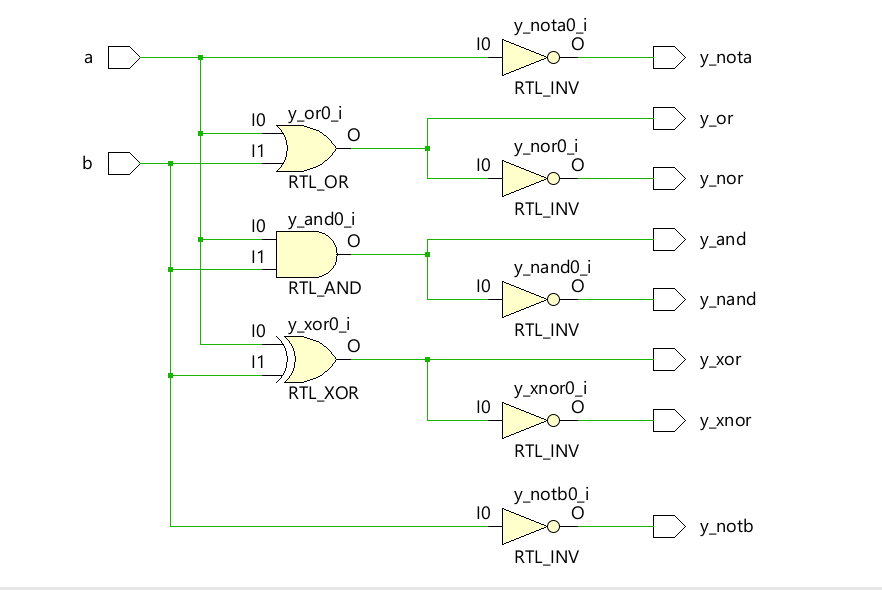
\includegraphics[width=0.9\textwidth]{5_rtl.png}
    \caption{RTL Schematic -- Basic Logic Gates Using Structural Modeling}
    \label{fig:5_rtl}
\end{figure}

%----------------------------------------
\section{Verilog Design Code}

\begin{verilogbox}
\begin{lstlisting}
`timescale 1ns/1ps

module gates (
    input  wire A,
    input  wire B,
    output wire Y_AND,
    output wire Y_OR,
    output wire Y_NOT,
    output wire Y_NAND,
    output wire Y_NOR,
    output wire Y_XOR,
    output wire Y_XNOR
);

    and  g1(Y_AND, A, B);
    or   g2(Y_OR, A, B);
    not  g3(Y_NOT, A);
    nand g4(Y_NAND, A, B);
    nor  g5(Y_NOR, A, B);
    xor  g6(Y_XOR, A, B);
    xnor g7(Y_XNOR, A, B);

endmodule
\end{lstlisting}
\end{verilogbox}

%----------------------------------------
\section{Testbench Code}

\begin{verilogbox}
\begin{lstlisting}
`timescale 1ns/1ps

module gates_tb;

    reg A, B;

    wire Y_AND;
    wire Y_OR;
    wire Y_NOT;
    wire Y_NAND;
    wire Y_NOR;
    wire Y_XOR;
    wire Y_XNOR;

    gates uut (
        .A(A),
        .B(B),
        .Y_AND(Y_AND),
        .Y_OR(Y_OR),
        .Y_NOT(Y_NOT),
        .Y_NAND(Y_NAND),
        .Y_NOR(Y_NOR),
        .Y_XOR(Y_XOR),
        .Y_XNOR(Y_XNOR)
    );

    integer i;

    initial begin

        $monitor("Time = %0t | A = %b | B = %b | AND = %b | OR = %b | NOT = %b | NAND = %b | NOR = %b | XOR = %b | XNOR = %b",
                 $time, A, B, Y_AND, Y_OR, Y_NOT,
                 Y_NAND, Y_NOR, Y_XOR, Y_XNOR);

        for (i = 0; i < 4; i = i + 1) begin
            {A, B} = i[1:0];
            #10;
        end

        $finish;
    end

endmodule
\end{lstlisting}
\end{verilogbox}

%----------------------------------------
\section{Simulation Results}

\begin{figure}[H]
    \centering
    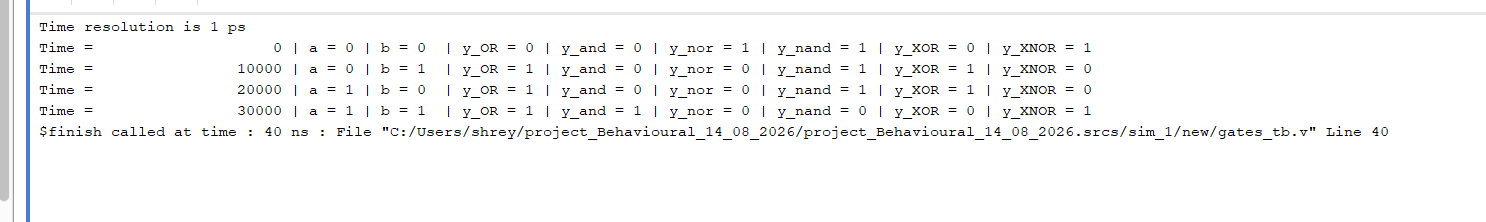
\includegraphics[width=1.0 \textwidth]{5_tcl.png}
    \caption{Truth table verification using TCL console}
    \label{fig:5_wave}
\end{figure}

\vspace{0.5cm}

\section{Results and Observations}

\begin{itemize}
    \item All seven logic gates were successfully implemented using Verilog HDL.
    \item The simulated outputs matched the expected truth table for all input combinations.
    \item The AND and NAND gates produced complementary outputs.
    \item The OR and NOR gates produced complementary outputs.
    \item XOR produced HIGH when the inputs were different, while XNOR produced HIGH when the inputs were equal.
\end{itemize}

\section{Conclusion}

The basic logic gates AND, OR, NOT, NAND, NOR, XOR, and XNOR were successfully implemented and verified using Verilog HDL. The simulation results matched the theoretical truth tables for all possible input combinations.

\section{Sources of Error}

\begin{itemize}
    \item Incorrect gate selection or signal connections may produce incorrect outputs.
    \item Incorrect input combinations in the testbench may result in incomplete verification.
    \item Errors in signal naming or module instantiation may cause compilation errors.
\end{itemize}


%----------------------------------------
\chapter{Implementation of a 4-to-1 Multiplexer}
\label{ch:pdf2}

\section{Objective}

To design and implement a \textbf{4-to-1 multiplexer} using Verilog HDL and verify its operation using appropriate select lines.

\section{Theory}

A multiplexer is a combinational circuit that selects one of several input signals and transfers the selected signal to a single output.

A 4-to-1 multiplexer consists of four data inputs $I_0$, $I_1$, $I_2$, and $I_3$, two select inputs $S_1$ and $S_0$, and one output $Y$.

The select lines determine which input is connected to the output.

\[
Y =
\begin{cases}
I_0, & S_1S_0=00\\
I_1, & S_1S_0=01\\
I_2, & S_1S_0=10\\
I_3, & S_1S_0=11
\end{cases}
\]

The Boolean expression is

\[
Y=\overline{S_1}\overline{S_0}I_0+
\overline{S_1}S_0I_1+
S_1\overline{S_0}I_2+
S_1S_0I_3.
\]

\section{Truth Table}

\begin{table}[H]
    \centering
    \begin{tabular}{|c|c|c|}
        \hline
        \textbf{$S_1$} & \textbf{$S_0$} & \textbf{Output $Y$} \\
        \hline
        0 & 0 & $I_0$ \\
        \hline
        0 & 1 & $I_1$ \\
        \hline
        1 & 0 & $I_2$ \\
        \hline
        1 & 1 & $I_3$ \\
        \hline
    \end{tabular}
    \caption{Truth table of a 4-to-1 multiplexer}
    \label{tab:4to1_mux}
\end{table}

\section{Software Tools}

Xilinx Vivado 2025.1 (Design Entry, RTL Analysis and Simulation)

\section{Procedure}

\begin{enumerate}
    \item Create a new RTL project in Xilinx Vivado.
    \item Define four data inputs, two select inputs, and one output.
    \item Implement the 4-to-1 multiplexer using Verilog HDL.
    \item Run RTL Analysis and generate the RTL schematic.
    \item Write a testbench to apply different input and select combinations.
    \item Perform behavioral simulation.
    \item Observe the waveform using GTKWave.
    \item Verify that the output corresponds to the selected input.
\end{enumerate}

%----------------------------------------
\section{RTL Diagram}

\begin{figure}[H]
    \centering
    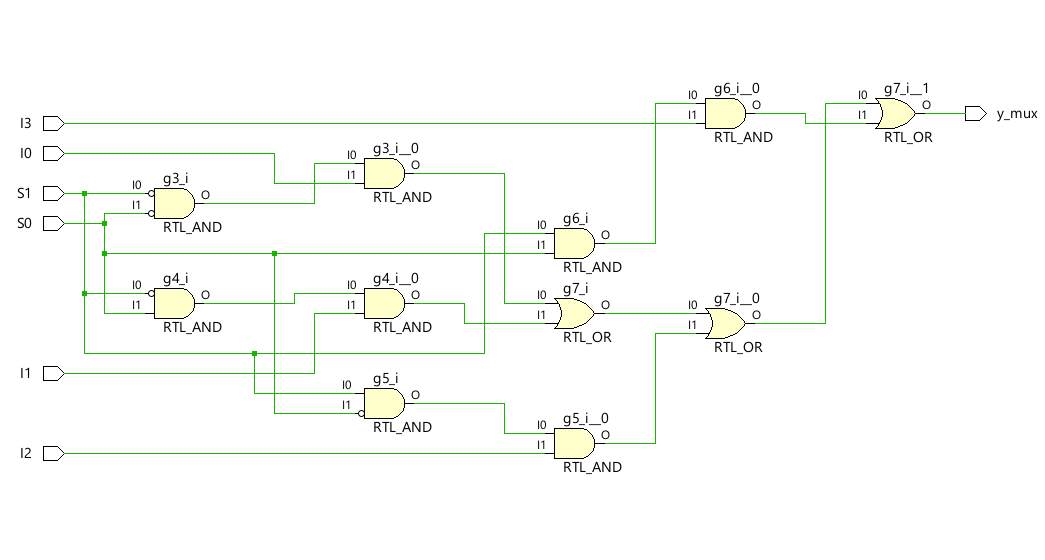
\includegraphics[width=0.9\textwidth]{images/6_rtl}
    \caption{RTL Schematic -- 4-to-1 Multiplexer Using Structural Modeling}
    \label{fig:6_rtl}
\end{figure}


%----------------------------------------
\section{Verilog Design Code}

\begin{verilogbox}
\begin{lstlisting}
`timescale 1ns/1ps

module mux4to1 (
    input  wire I0,
    input  wire I1,
    input  wire I2,
    input  wire I3,
    input  wire S0,
    input  wire S1,
    output wire Y
);

    assign Y = (~S1 & ~S0 & I0) |
               (~S1 &  S0 & I1) |
               ( S1 & ~S0 & I2) |
               ( S1 &  S0 & I3);

endmodule
\end{lstlisting}
\end{verilogbox}

%----------------------------------------
\section{Testbench Code}

\begin{verilogbox}
\begin{lstlisting}
`timescale 1ns/1ps

module mux4to1_tb;

    reg S0, S1;
    reg I0, I1, I2, I3;
    wire Y;

    mux4to1 uut (
        .S1(S1),
        .S0(S0),
        .I0(I0),
        .I1(I1),
        .I2(I2),
        .I3(I3),
        .Y(Y)
    );

    integer i;

    initial begin

        $monitor("Time = %0t | S1 = %b | S0 = %b | I0 = %b | I1 = %b | I2 = %b | I3 = %b | Y = %b",
                 $time, S1, S0, I0, I1, I2, I3, Y);

        I0 = 1'b0;
        I1 = 1'b1;
        I2 = 1'b0;
        I3 = 1'b1;

        for (i = 0; i < 4; i = i + 1) begin
            {S1, S0} = i[1:0];
            #10;
        end

        I0 = 1'b1;
        I1 = 1'b0;
        I2 = 1'b1;
        I3 = 1'b0;

        for (i = 0; i < 4; i = i + 1) begin
            {S1, S0} = i[1:0];
            #10;
        end

        $finish;
    end

endmodule
\end{lstlisting}
\end{verilogbox}

%----------------------------------------
\section{Simulation Results}

\begin{figure}[H]
    \centering
    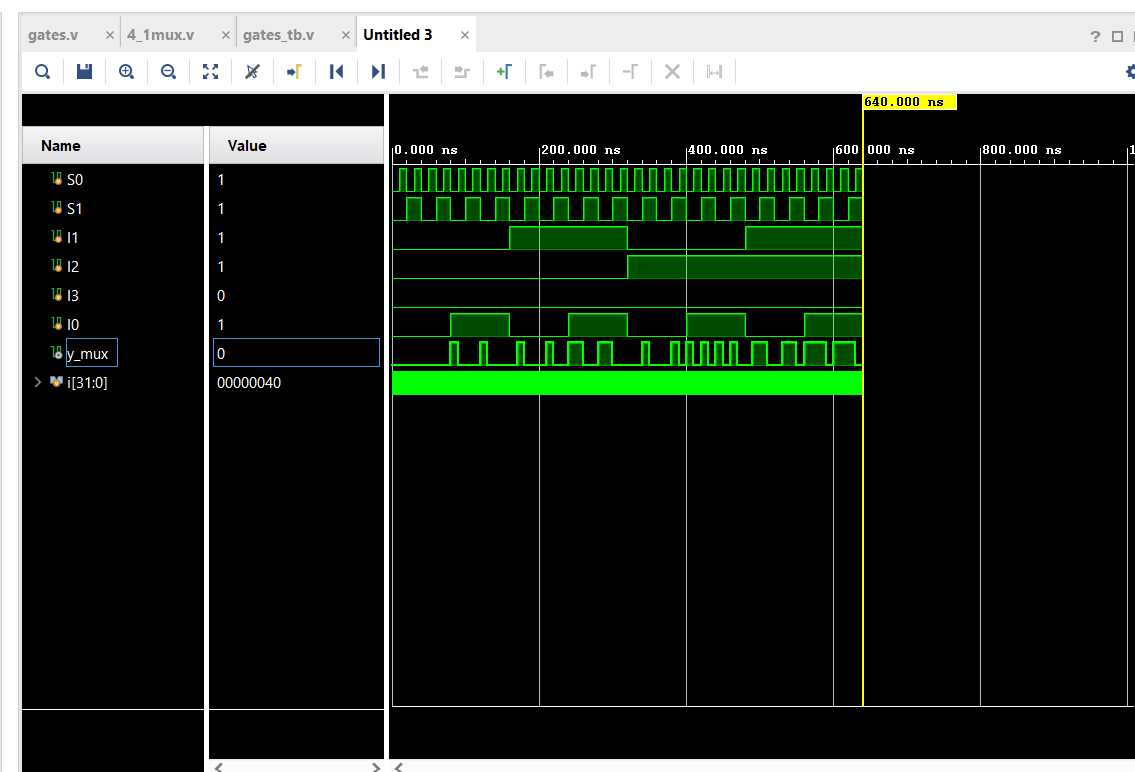
\includegraphics[width=0.95\textwidth]{images/6_wave}
    \caption{Simulation Waveform -- 4-to-1 Multiplexer Using Structural Modeling}
    \label{fig:6_wave}
\end{figure}


\vspace{0.5cm}

\section{Results and Observations}

\begin{itemize}
    \item The 4-to-1 multiplexer was successfully implemented using Verilog HDL.
    \item The select inputs correctly determine which data input appears at the output.
    \item For select combination 00, the output follows $I_0$.
    \item For select combination 01, the output follows $I_1$.
    \item For select combination 10, the output follows $I_2$.
    \item For select combination 11, the output follows $I_3$.
\end{itemize}

\section{Conclusion}

A 4-to-1 multiplexer was successfully designed and verified using Verilog HDL. The simulation results confirmed that the output correctly follows the data input selected by the two select lines.

\section{Sources of Error}

\begin{itemize}
    \item Incorrect mapping of select lines can result in selection of the wrong input.
    \item Incorrect Boolean expression may result in an incorrect output.
    \item Incomplete testbench combinations may leave some operating conditions unverified.
\end{itemize}


%----------------------------------------
\chapter{Implementation of a Single-Bit Full Adder}
\label{ch:pdf3}

\section{Objective}

To design and implement a \textbf{single-bit full adder} with inputs $A$, $B$, and $C_{in}$, producing Sum and Carry outputs using Verilog HDL.

\section{Theory}

A full adder is a combinational circuit that performs the addition of three single-bit binary inputs: $A$, $B$, and $C_{in}$.

It produces two outputs:

\begin{itemize}
    \item \textbf{Sum ($S$)} -- The least significant bit of the addition.
    \item \textbf{Carry ($C_{out}$)} -- The carry generated from the addition.
\end{itemize}

The Boolean expressions are

\[
S=A\oplus B\oplus C_{in}
\]

and

\[
C_{out}=AB+BC_{in}+AC_{in}.
\]


\section{Truth Table}

\begin{table}[H]
    \centering
    \begin{tabular}{|c|c|c|c|c|}
        \hline
        \textbf{A} & \textbf{B} & \textbf{$C_{in}$} & \textbf{Sum} & \textbf{$C_{out}$} \\
        \hline
        0 & 0 & 0 & 0 & 0 \\
        \hline
        0 & 0 & 1 & 1 & 0 \\
        \hline
        0 & 1 & 0 & 1 & 0 \\
        \hline
        0 & 1 & 1 & 0 & 1 \\
        \hline
        1 & 0 & 0 & 1 & 0 \\
        \hline
        1 & 0 & 1 & 0 & 1 \\
        \hline
        1 & 1 & 0 & 0 & 1 \\
        \hline
        1 & 1 & 1 & 1 & 1 \\
        \hline
    \end{tabular}
    \caption{Truth table of a single-bit full adder}
    \label{tab:full_adder}
\end{table}

\section{Software Tools}

Xilinx Vivado 2025.1 (Design Entry, RTL Analysis and Simulation), 

\section{Procedure}

\begin{enumerate}
    \item Create a new RTL project in Xilinx Vivado.
    \item Define inputs $A$, $B$, and $C_{in}$ and outputs Sum and $C_{out}$.
    \item Implement the full adder using Verilog HDL.
    \item Run RTL Analysis and generate the RTL schematic.
    \item Write a testbench to apply all eight possible input combinations.
    \item Run behavioral simulation.
    \item Observe the output waveforms.
    \item Verify the simulation results against the full-adder truth table.
\end{enumerate}

%----------------------------------------
\section{RTL Diagram}

\begin{figure}[H]
    \centering
    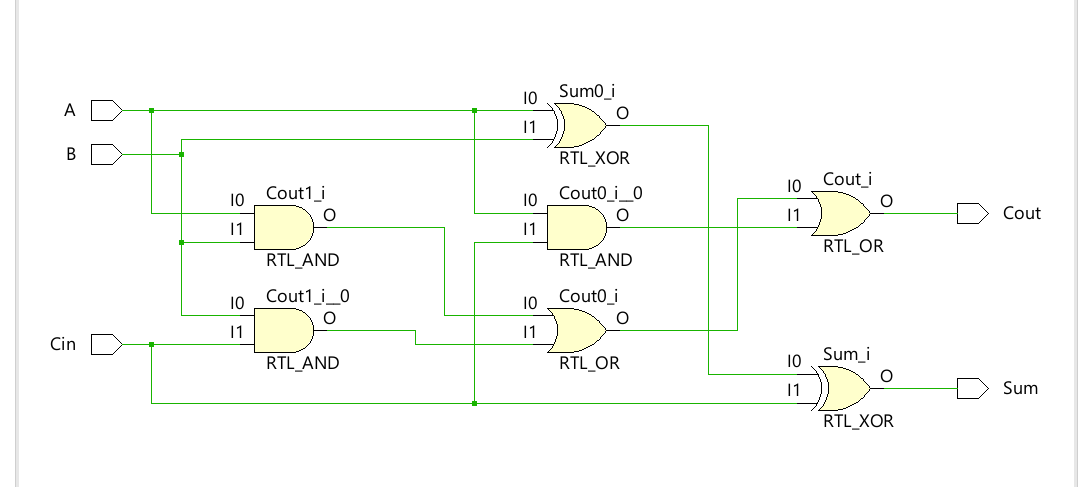
\includegraphics[width=0.9\textwidth]{images/3_rtl.png}
    \caption{RTL Schematic -- Implementation of a Single-Bit Full Adder}
    \label{fig:full_adder_rtl}
\end{figure}

%----------------------------------------
\section{Verilog Design Code}

\begin{verilogbox}
\begin{lstlisting}
`timescale 1ns/1ps

module full_adder (
    input  wire A,
    input  wire B,
    input  wire Cin,
    output wire Sum,
    output wire Cout
);

    assign Sum  = A ^ B ^ Cin;
    assign Cout = (A & B) | (B & Cin) | (A & Cin);

endmodule
\end{lstlisting}
\end{verilogbox}

%----------------------------------------
\section{Testbench Code}

\begin{verilogbox}
\begin{lstlisting}
`timescale 1ns/1ps

module full_adder_tb;

    reg A, B, Cin;
    wire Sum, Cout;

    full_adder uut (
        .A(A),
        .B(B),
        .Cin(Cin),
        .Sum(Sum),
        .Cout(Cout)
    );

    integer i;

    initial begin

        $monitor("Time = %0t | A = %b | B = %b | Cin = %b | Sum = %b | Cout = %b",
                 $time, A, B, Cin, Sum, Cout);

        for (i = 0; i < 8; i = i + 1) begin
            {A, B, Cin} = i[2:0];
            #10;
        end

        $finish;
    end

endmodule
\end{lstlisting}
\end{verilogbox}

%----------------------------------------
\section{Simulation Results}

\begin{figure}[H]
    \centering
    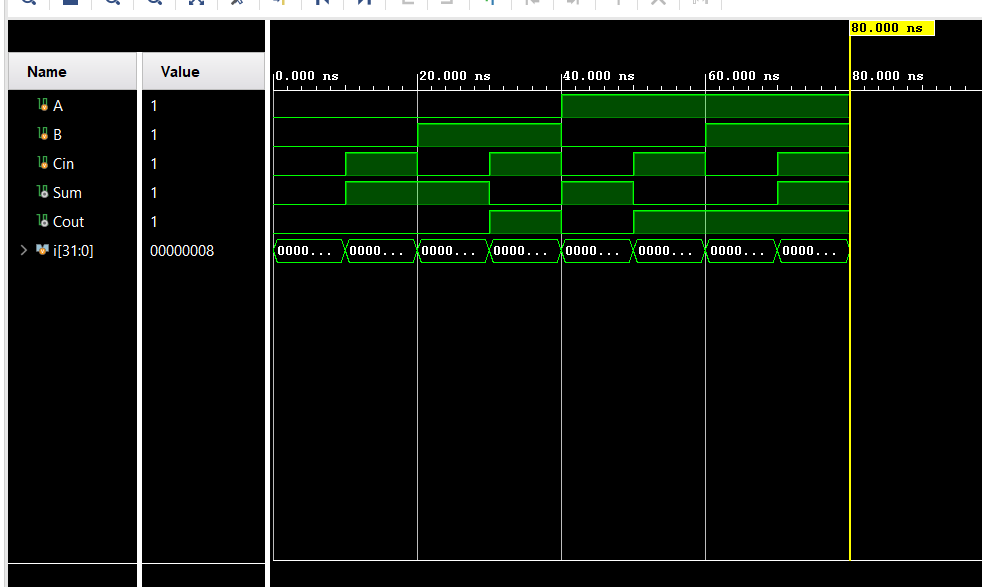
\includegraphics[width=0.95\textwidth]{images/3_gtkwave.png}
    \caption{Simulation Waveform -- Implementation of a Single-Bit Full Adder}
    \label{fig:full_adder_waveform}
\end{figure}

\begin{figure}[H]
    \centering
    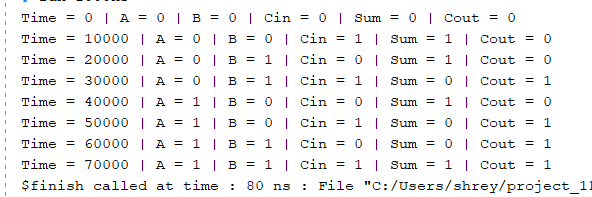
\includegraphics[width=0.95\textwidth]{images/3_sim.png}
    \caption{Truth table realization of a Single-Bit Full Adder}
    \label{fig:full_adder_waveform}
\end{figure}

\vspace{0.5cm}

\section{Results and Observations}

\begin{itemize}
    \item The single-bit full adder was successfully implemented using Verilog HDL.
    \item All eight possible combinations of $A$, $B$, and $C_{in}$ were verified.
    \item The Sum output follows the XOR relationship between the three inputs.
    \item The Carry output becomes HIGH whenever at least two of the three inputs are HIGH.
    \item The simulation results agree with the theoretical full-adder truth table.
\end{itemize}

\section{Conclusion}

A single-bit full adder was successfully designed and verified using Verilog HDL. The circuit correctly performs the addition of two binary bits along with an input carry and generates the corresponding Sum and Carry outputs.

\section{Sources of Error}

\begin{itemize}
    \item Incorrect implementation of the Sum or Carry Boolean expressions may produce incorrect results.
    \item Failure to test all eight input combinations may result in incomplete verification.
    \item Incorrect port connections between the testbench and design module may cause simulation errors.
\end{itemize}


%----------------------------------------
\chapter{Implementation of a Ripple Carry Adder}
\label{ch:pdf4}

\section{Objective}

To design and implement a \textbf{4-bit ripple carry adder} by connecting multiple single-bit full adders and verify its functionality using Verilog HDL.

\section{Theory}

A ripple carry adder (RCA) is a combinational circuit used to add two multi-bit binary numbers. It is constructed by connecting multiple full adders in cascade.

For a 4-bit ripple carry adder, four single-bit full adders are connected such that the carry output of one stage becomes the carry input of the next stage.

The addition is performed starting from the least significant bit (LSB). The carry generated at each stage propagates, or ``ripples'', toward the most significant bit (MSB).

For inputs

\[
A=A_3A_2A_1A_0
\]

and

\[
B=B_3B_2B_1B_0,
\]

the output is

\[
C_{out}S_3S_2S_1S_0=A+B+C_{in}.
\]

The carry propagation is given by

\[
C_1=f(A_0,B_0,C_0)
\]

\[
C_2=f(A_1,B_1,C_1)
\]

\[
C_3=f(A_2,B_2,C_2)
\]

\[
C_4=f(A_3,B_3,C_3).
\]

Here, $C_0$ is the input carry and $C_4$ is the final carry output.

\section{Truth Table}

Since the complete truth table of a 4-bit ripple carry adder contains $2^9=512$ input combinations, representative cases are shown below.

\begin{table}[H]
    \centering
    \begin{tabular}{|c|c|c|c|c|}
        \hline
        \textbf{A} & \textbf{B} & \textbf{$C_{in}$} & \textbf{Result} & \textbf{$C_{out}$} \\
        \hline
        0000 & 0000 & 0 & 0000 & 0 \\
        \hline
        0001 & 0001 & 0 & 0010 & 0 \\
        \hline
        0011 & 0010 & 0 & 0101 & 0 \\
        \hline
        0101 & 0011 & 0 & 1000 & 0 \\
        \hline
        0111 & 0001 & 0 & 1000 & 0 \\
        \hline
        1111 & 0001 & 0 & 0000 & 1 \\
        \hline
        1010 & 0101 & 1 & 0000 & 1 \\
        \hline
        1111 & 1111 & 0 & 1110 & 1 \\
        \hline
    \end{tabular}
    \caption{Representative truth table of a 4-bit ripple carry adder}
    \label{tab:ripple_carry_adder}
\end{table}

\section{Software Tools}

Xilinx Vivado 2025.1 (Design Entry, RTL Analysis and Simulation)
\section{Procedure}

\begin{enumerate}
    \item Create a new RTL project in Xilinx Vivado.
    \item Design a single-bit full adder module.
    \item Instantiate four full adders to construct the 4-bit ripple carry adder.
    \item Connect the carry output of each stage to the carry input of the following stage.
    \item Apply two 4-bit binary inputs and an input carry.
    \item Run RTL Analysis and generate the RTL schematic.
    \item Write a testbench containing representative addition cases.
    \item Perform behavioral simulation.
    \item Observe the waveform using GTKWave.
    \item Verify the calculated sum and final carry output.
\end{enumerate}

%----------------------------------------
\section{RTL Diagram}

\begin{figure}[H]
    \centering
    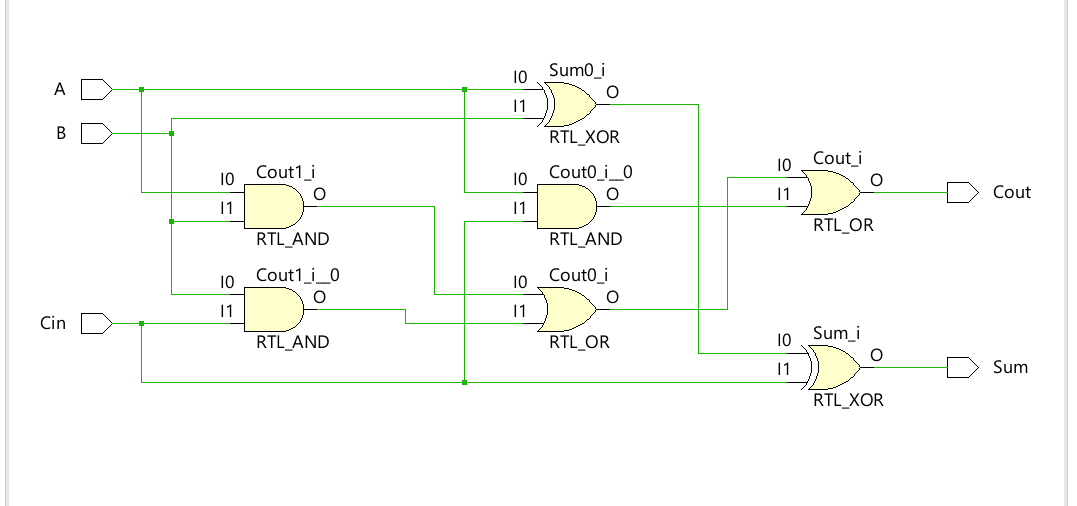
\includegraphics[width=1.1\textwidth]{images/4_rtl.png}
    \caption{RTL Schematic -- Implementation of a 4-bit Ripple Carry Adder}
    \label{fig:ripple_adder_rtl}
\end{figure}

%----------------------------------------
\section{Verilog Design Code}

\begin{verilogbox}
\begin{lstlisting}
`timescale 1ns/1ps

module full_adder (
    input  wire A,
    input  wire B,
    input  wire Cin,
    output wire Sum,
    output wire Cout
);

    assign Sum  = A ^ B ^ Cin;
    assign Cout = (A & B) | (B & Cin) | (A & Cin);

endmodule


module ripple_carry_adder (
    input  wire [3:0] A,
    input  wire [3:0] B,
    input  wire       Cin,
    output wire [3:0] Sum,
    output wire       Cout
);

    wire C1, C2, C3;

    full_adder FA0 (
        .A(A[0]),
        .B(B[0]),
        .Cin(Cin),
        .Sum(Sum[0]),
        .Cout(C1)
    );

    full_adder FA1 (
        .A(A[1]),
        .B(B[1]),
        .Cin(C1),
        .Sum(Sum[1]),
        .Cout(C2)
    );

    full_adder FA2 (
        .A(A[2]),
        .B(B[2]),
        .Cin(C2),
        .Sum(Sum[2]),
        .Cout(C3)
    );

    full_adder FA3 (
        .A(A[3]),
        .B(B[3]),
        .Cin(C3),
        .Sum(Sum[3]),
        .Cout(Cout)
    );

endmodule
\end{lstlisting}
\end{verilogbox}

%----------------------------------------
\section{Testbench Code}

\begin{verilogbox}
\begin{lstlisting}
`timescale 1ns/1ps

module ripple_carry_adder_tb;

    reg  [3:0] A, B;
    reg        Cin;

    wire [3:0] Sum;
    wire       Cout;

    ripple_carry_adder uut (
        .A(A),
        .B(B),
        .Cin(Cin),
        .Sum(Sum),
        .Cout(Cout)
    );

    initial begin

        $monitor("Time = %0t | A = %b | B = %b | Cin = %b | Sum = %b | Cout = %b",
                 $time, A, B, Cin, Sum, Cout);

        A = 4'b0000;
        B = 4'b0000;
        Cin = 1'b0;
        #10;

        A = 4'b0001;
        B = 4'b0001;
        Cin = 1'b0;
        #10;

        A = 4'b0011;
        B = 4'b0010;
        Cin = 1'b0;
        #10;

        A = 4'b0101;
        B = 4'b0011;
        Cin = 1'b0;
        #10;

        A = 4'b0111;
        B = 4'b0001;
        Cin = 1'b0;
        #10;

        A = 4'b1111;
        B = 4'b0001;
        Cin = 1'b0;
        #10;

        A = 4'b1010;
        B = 4'b0101;
        Cin = 1'b1;
        #10;

        A = 4'b1111;
        B = 4'b1111;
        Cin = 1'b0;
        #10;

        $finish;
    end

endmodule
\end{lstlisting}
\end{verilogbox}

%----------------------------------------
\section{Simulation Results}

\begin{figure}[H]
    \centering
    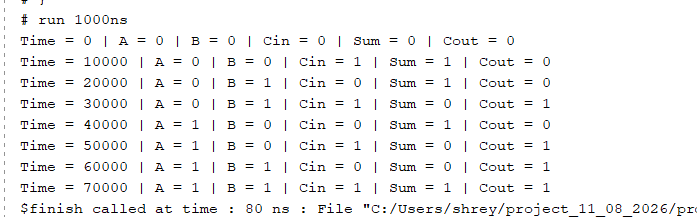
\includegraphics[width=0.95\textwidth]{images/4_sim.png}
    \caption{Simulation Waveform -- Implementation of a 4-bit Ripple Carry Adder}
    \label{fig:ripple_adder_waveform}
\end{figure} 



\vspace{0.5cm}

\section{Results and Observations}

\begin{itemize}
    \item A 4-bit ripple carry adder was successfully constructed using four single-bit full adders.
    \item The carry output of each full-adder stage is connected to the carry input of the next stage.
    \item The circuit correctly performs binary addition of two 4-bit numbers along with the input carry.
    \item The final carry output indicates overflow beyond the 4-bit result.
    \item The simulation results matched the expected arithmetic results for all applied test cases.
\end{itemize}

\section{Conclusion}

A 4-bit ripple carry adder was successfully designed by cascading four single-bit full adders. The design correctly performs binary addition and propagates the carry from the least significant bit toward the most significant bit. The functionality was verified through RTL simulation.

\section{Sources of Error}

\begin{itemize}
    \item Incorrect connection of carry signals between consecutive full-adder stages may produce incorrect results.
    \item Incorrect bit ordering can cause errors in the calculated sum.
    \item Failure to account for the final carry may result in an incomplete interpretation of the addition.
    \item Incomplete test cases may fail to verify carry propagation through all four stages.
\end{itemize}
%----------------------------------------
%----------------------------------------
\chapter{Implementation of Basic Logic Gates Using Structural Modeling}
\label{ch:pdf13}

\section{Objective}

To design and implement basic logic gates using structural modeling in Verilog HDL and verify their functionality through simulation.

\section{Theory}

Structural modeling in Verilog HDL describes a digital circuit by explicitly instantiating logic gates and connecting them to form the required circuit.

In this experiment, the basic logic gates AND, OR, NOT, NAND, NOR, XOR, and XNOR are implemented using Verilog's built-in gate primitives.

The Boolean expressions for the respective gates are:

\[
Y_{AND} = A \cdot B
\]

\[
Y_{OR} = A + B
\]

\[
Y_{NOT} = \overline{A}
\]

\[
Y_{NAND} = \overline{A \cdot B}
\]

\[
Y_{NOR} = \overline{A + B}
\]

\[
Y_{XOR} = A \oplus B
\]

\[
Y_{XNOR} = \overline{A \oplus B}
\]

The circuit is constructed by directly instantiating the corresponding Verilog gate primitives such as \texttt{and}, \texttt{or}, \texttt{not}, \texttt{nand}, \texttt{nor}, \texttt{xor}, and \texttt{xnor}.

\section{Truth Table}

\begin{table}[H]
    \centering
    \caption{Truth Table of Basic Logic Gates}
    \label{tab:basic_gates_structural}
    \begin{tabular}{|c|c|c|c|c|c|c|c|}
    \hline
    \textbf{A} & \textbf{B} & \textbf{AND} & \textbf{OR} &
    \textbf{NAND} & \textbf{NOR} & \textbf{XOR} & \textbf{XNOR} \\
    \hline
    0 & 0 & 0 & 0 & 1 & 1 & 0 & 1 \\
    \hline
    0 & 1 & 0 & 1 & 1 & 0 & 1 & 0 \\
    \hline
    1 & 0 & 0 & 1 & 1 & 0 & 1 & 0 \\
    \hline
    1 & 1 & 1 & 1 & 0 & 0 & 0 & 1 \\
    \hline
    \end{tabular}
\end{table}

For the NOT gate:

\begin{table}[H]
    \centering
    \caption{Truth Table of NOT Gate}
    \label{tab:not_structural}
    \begin{tabular}{|c|c|}
    \hline
    \textbf{A} & \textbf{NOT A} \\
    \hline
    0 & 1 \\
    \hline
    1 & 0 \\
    \hline
    \end{tabular}
\end{table}

\section{Software Tools}

Xilinx Vivado 2025.1 (Design Entry, RTL Analysis and Simulation)

\section{Procedure}

\begin{enumerate}
    \item Create a new RTL project in Vivado.
    \item Define the required input and output signals for the logic gates.
    \item Write the Verilog module using structural modeling.
    \item Instantiate the required Verilog gate primitives.
    \item Connect the gates to obtain the required logic functions.
    \item Run RTL Analysis and generate the RTL schematic.
    \item Write a testbench to apply all possible combinations of the input signals.
    \item Run the behavioral simulation.
    \item Verify the simulated outputs against the corresponding truth tables.
\end{enumerate}

%----------------------------------------
\section{RTL Diagram}

\begin{figure}[H]
    \centering
    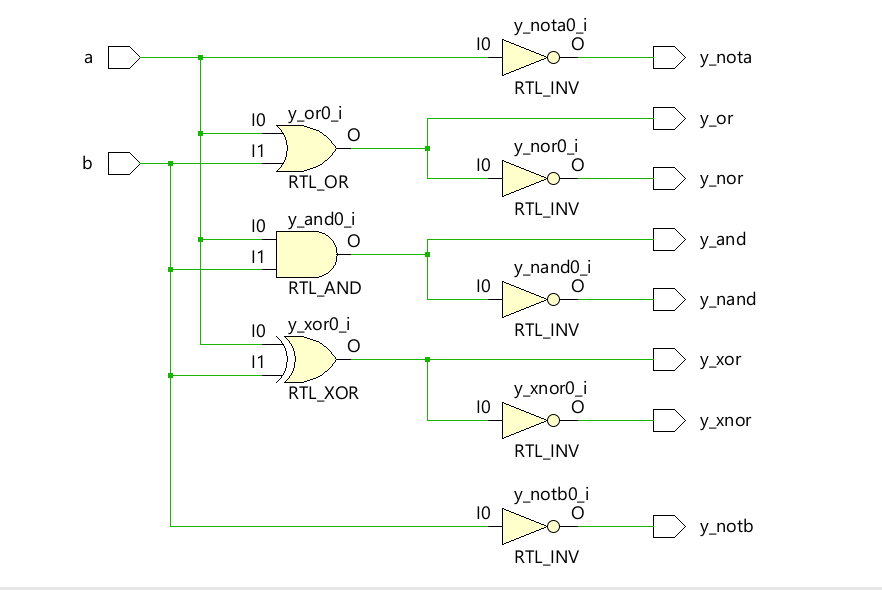
\includegraphics[width=0.9\textwidth]{5_rtl.png}
    \caption{RTL Schematic -- Basic Logic Gates Using Structural Modeling}
    \label{fig:5_rtl}
\end{figure}

%----------------------------------------
\section{Verilog Design Code}

\begin{verilogbox}
\begin{lstlisting}
module gates(
    input A,
    input B,
    output Y_AND,
    output Y_OR,
    output Y_NOT,
    output Y_NAND,
    output Y_NOR,
    output Y_XOR,
    output Y_XNOR
);

    and  g1(Y_AND, A, B);
    or   g2(Y_OR, A, B);
    not  g3(Y_NOT, A);
    nand g4(Y_NAND, A, B);
    nor  g5(Y_NOR, A, B);
    xor  g6(Y_XOR, A, B);
    xnor g7(Y_XNOR, A, B);

endmodule
\end{lstlisting}
\end{verilogbox}

%----------------------------------------
\section{Testbench Code}

\begin{verilogbox}
\begin{lstlisting}
module gates_tb;

    reg A, B;

    wire Y_AND;
    wire Y_OR;
    wire Y_NOT;
    wire Y_NAND;
    wire Y_NOR;
    wire Y_XOR;
    wire Y_XNOR;

    gates uut (
        .A(A),
        .B(B),
        .Y_AND(Y_AND),
        .Y_OR(Y_OR),
        .Y_NOT(Y_NOT),
        .Y_NAND(Y_NAND),
        .Y_NOR(Y_NOR),
        .Y_XOR(Y_XOR),
        .Y_XNOR(Y_XNOR)
    );

    integer i;

    initial begin

        $monitor("Time = %0t | A = %b | B = %b | AND = %b | OR = %b | NOT = %b | NAND = %b | NOR = %b | XOR = %b | XNOR = %b",
                 $time, A, B, Y_AND, Y_OR, Y_NOT,
                 Y_NAND, Y_NOR, Y_XOR, Y_XNOR);

        for (i = 0; i < 4; i = i + 1) begin
            {A, B} = i[1:0];
            #10;
        end

        $finish;

    end

endmodule
\end{lstlisting}
\end{verilogbox}

%----------------------------------------
\section{Simulation Results}

\begin{figure}[H]
    \centering
    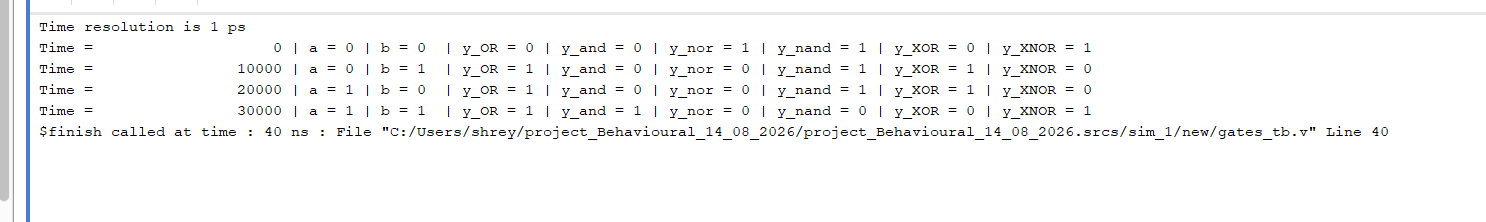
\includegraphics[width=1.0 \textwidth]{5_tcl.png}
    \caption{Truth table verification using TCL console}
    \label{fig:5_wave}
\end{figure}

\vspace{0.5cm}

\section{Results and Observations}

The basic logic gates were successfully implemented using structural modeling in Verilog HDL. The required gate primitives were instantiated and interconnected to implement AND, OR, NOT, NAND, NOR, XOR, and XNOR operations.

All possible combinations of the input signals were applied during simulation. The observed outputs were found to be consistent with the corresponding truth tables, verifying the correct operation of the implemented logic gates.

\vspace{2cm}

\section{Conclusion}

The basic logic gates were successfully designed and implemented using structural modeling in Verilog HDL. The experiment demonstrated the use of Verilog gate primitives to describe digital circuits by explicitly specifying their structural interconnections. The simulation results verified the correct functionality of all implemented logic gates.

\vspace{1.5cm}

\section{Sources of Error}

\begin{itemize}
    \item Incorrect selection or instantiation of gate primitives may result in incorrect outputs.
    \item Incorrect connections between the gates and input signals may cause unexpected results.
    \item Uninitialized input signals may produce unknown (\texttt{X}) values during simulation.
    \item Errors in the testbench input sequence may result in incomplete verification.
    \item Incorrect module connections or port assignments may cause compilation or simulation errors.
\end{itemize}

\vspace{2.5cm}
%----------------------------------------
\chapter{Implementation of a 4-to-1 Multiplexer Using Structural Modeling}
\label{ch:pdf12}

\section{Objective}

To design and implement a \textbf{4-to-1 Multiplexer} using structural modeling in Verilog HDL and verify its functionality through simulation.

\section{Theory}

A 4-to-1 multiplexer is a combinational circuit that selects one of four input signals and transfers the selected input to a single output based on two select lines.

The multiplexer consists of four data inputs $I_0$, $I_1$, $I_2$, and $I_3$, two select lines $S_1$ and $S_0$, and one output $Y$.

The Boolean expression for a 4-to-1 multiplexer is:

\[
Y =
\overline{S_1}\overline{S_0}I_0
+
\overline{S_1}S_0I_1
+
S_1\overline{S_0}I_2
+
S_1S_0I_3
\]

In structural modeling, the circuit is described by explicitly instantiating logic gates and connecting them together. The design therefore represents the actual hardware structure of the circuit.

For the 4-to-1 multiplexer, NOT, AND, and OR gates are used to implement the required Boolean expression.

\section{Truth Table}

\begin{table}[H]
    \centering
    \caption{Truth Table of 4-to-1 Multiplexer}
    \label{tab:mux4_structural}
    \begin{tabular}{|c|c|c|}
    \hline
    \textbf{$S_1$} & \textbf{$S_0$} & \textbf{Output $Y$} \\
    \hline
    0 & 0 & $I_0$ \\
    \hline
    0 & 1 & $I_1$ \\
    \hline
    1 & 0 & $I_2$ \\
    \hline
    1 & 1 & $I_3$ \\
    \hline
    \end{tabular}
\end{table}

\section{Software Tools}

Xilinx Vivado 2025.1 (Design Entry, RTL Analysis and Simulation)

\section{Procedure}

\begin{enumerate}
    \item Create a new RTL project in Vivado.
    \item Define four data inputs $I_0$--$I_3$, two select inputs $S_1$ and $S_0$, and output $Y$.
    \item Write the Verilog module using structural modeling.
    \item Instantiate the required NOT, AND, and OR gates.
    \item Connect the gates according to the Boolean expression of the 4-to-1 multiplexer.
    \item Run RTL Analysis and generate the RTL schematic.
    \item Write a testbench to apply different combinations of data and select inputs.
    \item Run the behavioral simulation and view the waveform in GTKWave.
    \item Verify the output against the expected truth table.
\end{enumerate}

%----------------------------------------
\section{RTL Diagram}

\begin{figure}[H]
    \centering
    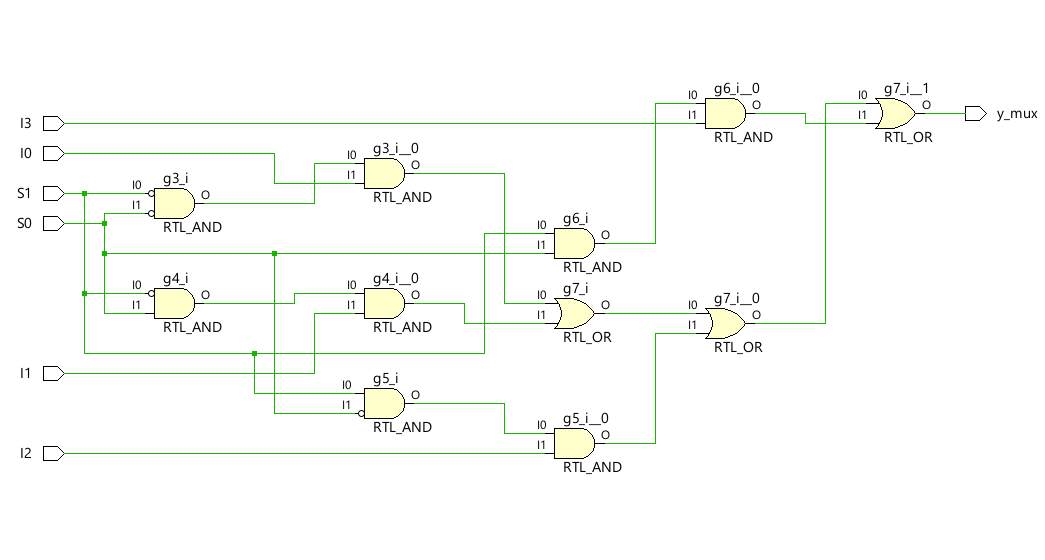
\includegraphics[width=0.9\textwidth]{images/6_rtl}
    \caption{RTL Schematic -- 4-to-1 Multiplexer Using Structural Modeling}
    \label{fig:6_rtl}
\end{figure}

%----------------------------------------
\section{Verilog Design Code}

\begin{verilogbox}
\begin{lstlisting}
module gates(
    input S1, S0, I0, I1, I2, I3,
    output y_mux
);

    wire S1_not, S0_not;
    wire y_and1, y_and2, y_and3, y_and4;

    not g1(S1_not, S1);
    not g2(S0_not, S0);

    and g3(y_and1, S1_not, S0_not, I0);
    and g4(y_and2, S1_not, S0, I1);
    and g5(y_and3, S1, S0_not, I2);
    and g6(y_and4, S1, S0, I3);

    or g7(y_mux, y_and1, y_and2, y_and3, y_and4);

endmodule
\end{lstlisting}
\end{verilogbox}

%----------------------------------------
\section{Testbench Code}

\begin{verilogbox}
\begin{lstlisting}
module gates_tb_mux;

    reg S0, S1, I0, I1, I2, I3;
    wire y_mux;

    gates uut (
        .S1(S1),
        .S0(S0),
        .I0(I0),
        .I1(I1),
        .I2(I2),
        .I3(I3),
        .y_mux(y_mux)
    );

    integer i;

    initial begin

        $monitor("Time = %0t | S1 = %b | S0 = %b | I0 = %b | I1 = %b | I2 = %b | I3 = %b | Y = %b",
                 $time, S1, S0, I0, I1, I2, I3, y_mux);

        for (i = 0; i < 64; i = i + 1) begin
            {S1, S0, I3, I2, I1, I0} = i[5:0];
            #10;
        end

        $finish;

    end

endmodule
\end{lstlisting}
\end{verilogbox}

%----------------------------------------
\section{Simulation Results}

\begin{figure}[H]
    \centering
    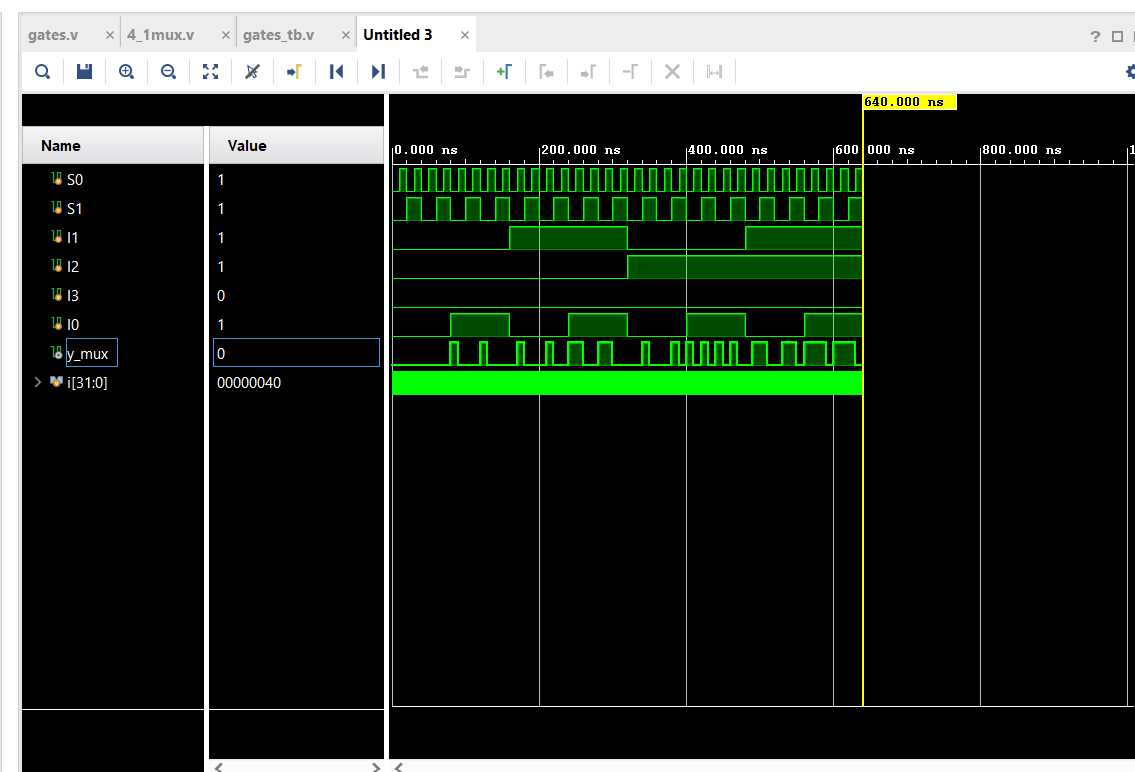
\includegraphics[width=0.95\textwidth]{images/6_wave}
    \caption{Simulation Waveform -- 4-to-1 Multiplexer Using Structural Modeling}
    \label{fig:6_wave}
\end{figure}

\vspace{0.5cm}

\section{Results and Observations}

The 4-to-1 multiplexer was successfully implemented using structural modeling in Verilog HDL. The required NOT, AND, and OR gates were instantiated and interconnected according to the Boolean expression of the multiplexer.

The simulation verified that the output $Y$ correctly follows the selected input for all possible combinations of the select lines. The observed results were consistent with the expected truth table.

\vspace{2cm}

\section{Conclusion}

A 4-to-1 multiplexer was successfully designed and implemented using structural modeling in Verilog HDL. The circuit was constructed using basic logic gates, demonstrating how a higher-level combinational circuit can be represented by explicitly connecting its constituent gates. The simulation results verified the correct operation of the multiplexer.

\vspace{1.5cm}

\section{Sources of Error}

\begin{itemize}
    \item Incorrect interconnection of the instantiated logic gates may result in an incorrect output.
    \item Errors in the Boolean expression may lead to incorrect multiplexer operation.
    \item Incorrect assignment of the select inputs may cause the wrong data input to be selected.
    \item Uninitialized signals may produce unknown (\texttt{X}) values during simulation.
    \item Errors in the testbench input sequence may result in incomplete verification.
    \item Incorrect module connections or port assignments may cause compilation or simulation errors.
\end{itemize}

\vspace{2.5cm}


%----------------------------------------
%----------------------------------------
\chapter{Implementation of a Full Subtractor}
\label{ch:pdf11}

\section{Objective}

To design and implement a \textbf{Full Subtractor} using Verilog HDL with inputs $A$, $B$, and $B_{in}$, producing Difference and Borrow outputs, and verify its functionality through simulation.

\section{Theory}

A full subtractor is a combinational digital circuit that performs the subtraction of three binary inputs. The three inputs are the minuend $A$, subtrahend $B$, and borrow-in $B_{in}$.

The circuit produces two outputs:

\begin{itemize}
    \item Difference ($D$)
    \item Borrow-out ($B_{out}$)
\end{itemize}

The Difference output is given by:

\[
D = A \oplus B \oplus B_{in}
\]

The Borrow-out output is given by:

\[
B_{out} = \overline{A}B + \overline{A}B_{in} + BB_{in}
\]

The full subtractor performs the operation:

\[
A - B - B_{in}
\]

The Difference represents the resulting binary difference, while the Borrow-out indicates whether a borrow is required from the next higher-order bit.

\section{Truth Table}

\begin{table}[H]
    \centering
    \caption{Truth Table of Full Subtractor}
    \label{tab:full_subtractor}
    \begin{tabular}{|c|c|c|c|c|}
    \hline
    \textbf{A} & \textbf{B} & \textbf{$B_{in}$} &
    \textbf{Difference} & \textbf{$B_{out}$} \\
    \hline
    0 & 0 & 0 & 0 & 0 \\
    \hline
    0 & 0 & 1 & 1 & 1 \\
    \hline
    0 & 1 & 0 & 1 & 1 \\
    \hline
    0 & 1 & 1 & 0 & 1 \\
    \hline
    1 & 0 & 0 & 1 & 0 \\
    \hline
    1 & 0 & 1 & 0 & 0 \\
    \hline
    1 & 1 & 0 & 0 & 0 \\
    \hline
    1 & 1 & 1 & 1 & 1 \\
    \hline
    \end{tabular}
\end{table}

\section{Software Tools}

Xilinx Vivado 2025.1 (Design Entry, RTL Analysis and Simulation)

\section{Procedure}

\begin{enumerate}
    \item Create a new RTL project in Vivado.
    \item Define the inputs $A$, $B$, and $B_{in}$ and the outputs Difference and $B_{out}$.
    \item Write the Verilog module for the full subtractor.
    \item Implement the Difference and Borrow-out Boolean expressions.
    \item Run RTL Analysis and generate the RTL schematic.
    \item Write a testbench to apply all possible combinations of the three inputs.
    \item Run the behavioral simulation.
    \item View the generated waveform .
    \item Verify the simulated outputs with the expected truth table.
\end{enumerate}

%----------------------------------------
\section{RTL Diagram}
\begin{figure}
    \centering
    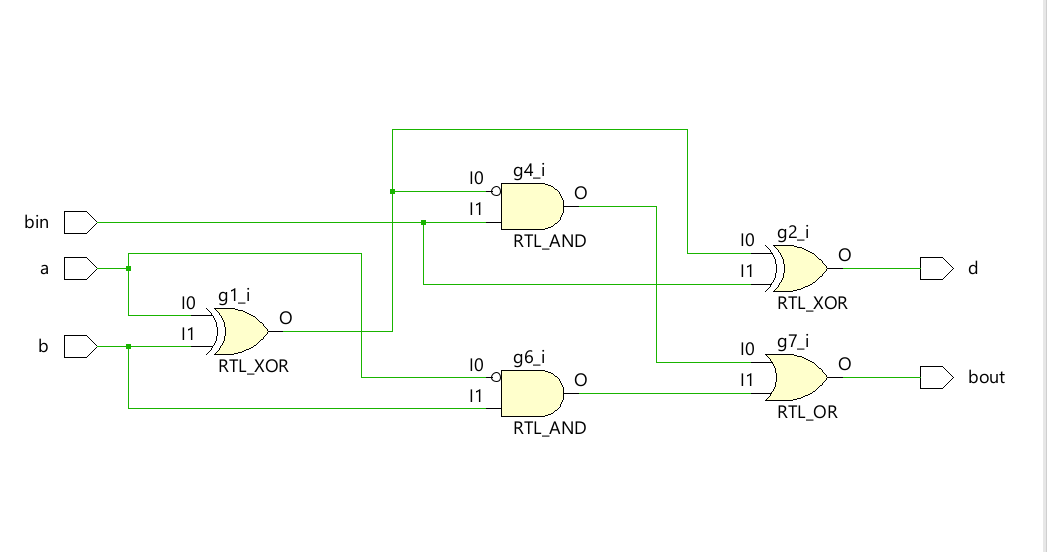
\includegraphics[width=1.0\linewidth]{images/7_rtl.png}
   \caption{RTL Schematic -- Implementation of Full Subtractor}
    \label{fig:placeholder}
\end{figure}


%----------------------------------------
\section{Verilog Design Code}

\begin{verilogbox}
\begin{lstlisting}

module sub(
    input a,
    input b,
    input bin,
    output d,
    output bout
);

    wire y1, y2, y3, y8, abar;

    // Difference
    xor g1(y1, a, b);
    xor g2(d, y1, bin);

    // Borrow
    not g3(y2, y1);
    and g4(y8, y2, bin);

    not g5(abar, a);

    and g6(y3, abar, b);
    or  g7(bout, y8, y3);

endmodule
\end{lstlisting}
\end{verilogbox}

%----------------------------------------
\section{Testbench Code}

\begin{verilogbox}
\begin{lstlisting}

module sub_tb(

);

	reg a,b,bin;
	wire bout,d;
	sub uut ( a, b , bin, bout , d );
	integer i;
	
	initial begin
          
          $monitor("Time = %t | a = %b | b = %b  | bin = %b | d = %b | bout = %b ",$time,a,b,bin,d,bout);
          for (i=0; i<8; i=i+1) 
          begin
           {a,b,bin} = i[2:0];
           #10;
          end
          $finish;
        end
endmodule
\end{lstlisting}
\end{verilogbox}

%----------------------------------------
\section{Simulation Results}
\begin{figure}
    \centering
    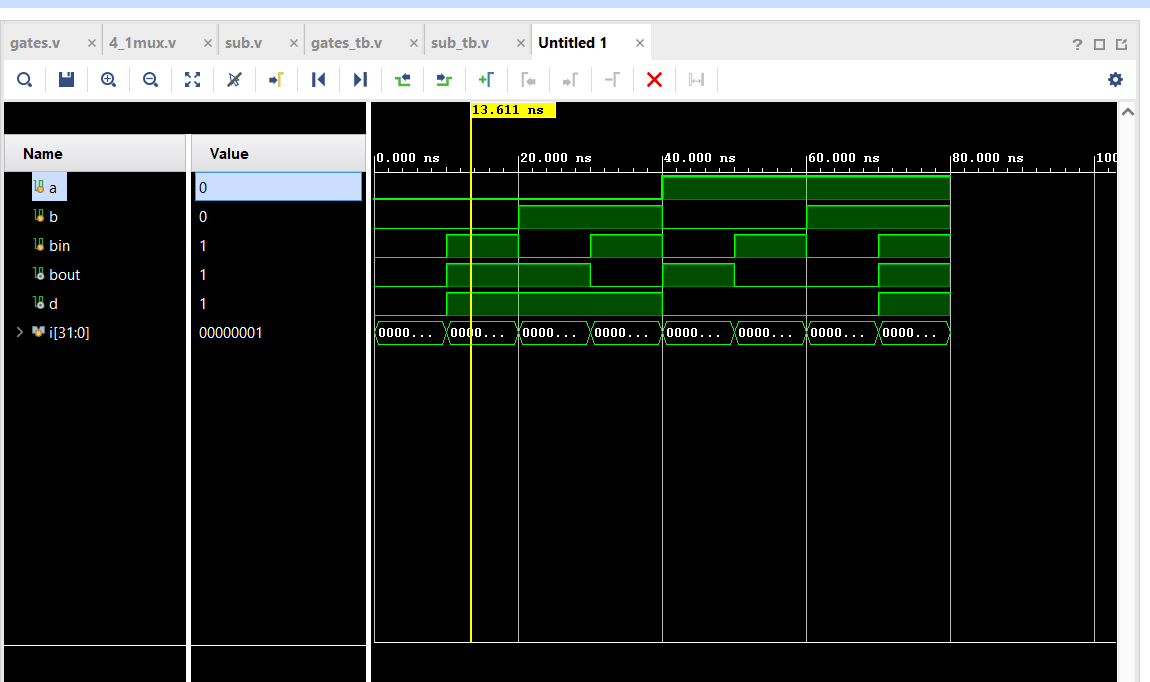
\includegraphics[width=1.0\linewidth]{images/7_wave.png}
    \caption{Simulation Waveform -- Implementation of Full Subtractor}
    \label{fig:placeholder}
\end{figure}
\begin{figure}
    \centering
    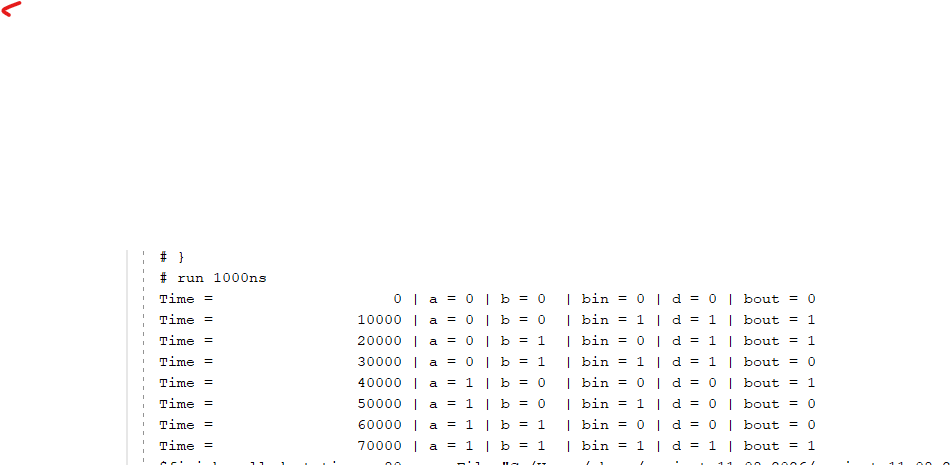
\includegraphics[width=1.0\linewidth]{images/7_tcl.png}
    \caption{TCL console of Truth table of Full subtractor}
    \label{fig:placeholder}
\end{figure}

\section{Results and Observations}

The full subtractor was successfully designed and implemented using Verilog HDL. All eight possible combinations of the inputs $A$, $B$, and $B_{in}$ were applied during simulation.

The observed Difference and Borrow-out outputs were found to be consistent with the expected truth table. The circuit correctly performs the binary subtraction operation while generating the appropriate borrow when required.


\section{Conclusion}

A full subtractor was successfully designed, implemented, and simulated using Verilog HDL. The circuit correctly generates the Difference and Borrow-out outputs for all possible combinations of the input signals. The simulation results verified the proper functionality of the designed full subtractor.



\section{Sources of Error}

\begin{itemize}
    \item Incorrect implementation of the Difference or Borrow-out Boolean expressions may result in incorrect outputs.
    \item Incorrect assignment of the borrow-in signal can affect both the Difference and Borrow-out outputs.
    \item Errors in the testbench input sequence may result in incomplete verification.
    \item Improper module connections may lead to incorrect simulation results.
    \item Uninitialized input signals may produce unknown (\texttt{X}) values during simulation.
\end{itemize}


%----------------------------------------
\chapter{Realization of Logic Gates using Behavioral Modelling}
\label{ch:pdf8}

\section{Objective}

To design and verify the basic logic gates (AND, OR, NOT, NAND, NOR, XOR, XNOR) using \textbf{Behavioral Modelling} using Verilog HDL and validate its functionality through simulation.

\section{Theory}

Behavioral modeling in Verilog HDL describes the behavior of a digital circuit using procedural statements inside an \texttt{always} block. Unlike gate-level modeling, behavioral modeling focuses on the desired operation of the circuit rather than explicitly describing the individual gates.

In this experiment, the basic logic gates AND, OR, NOT, NAND, NOR, XOR, and XNOR are implemented using behavioral modeling.

The corresponding Boolean expressions are:

\[
Y_{AND} = A \cdot B
\]

\[
Y_{OR} = A + B
\]

\[
Y_{NOT} = \overline{A}
\]

\[
Y_{NAND} = \overline{A \cdot B}
\]

\[
Y_{NOR} = \overline{A + B}
\]

\[
Y_{XOR} = A \oplus B
\]

\[
Y_{XNOR} = \overline{A \oplus B}
\]

The outputs are assigned inside a procedural \texttt{always @(*)} block. The \texttt{@(*)} sensitivity list ensures that the outputs are recalculated whenever any of the input signals changes.

\section{Truth Table}

\begin{table}[H]
    \centering
    \caption{Truth Table of Basic Logic Gates}
    \label{tab:basic_gates}
    \begin{tabular}{|c|c|c|c|c|c|c|c|c|c|}
    \hline
    \textbf{A} & \textbf{B} & \textbf{AND} & \textbf{OR} &
    \textbf{NAND} & \textbf{NOR} & \textbf{XOR} & \textbf{XNOR} \\
    \hline
    0 & 0 & 0 & 0 & 1 & 1 & 0 & 1 \\
    \hline
    0 & 1 & 0 & 1 & 1 & 0 & 1 & 0 \\
    \hline
    1 & 0 & 0 & 1 & 1 & 0 & 1 & 0 \\
    \hline
    1 & 1 & 1 & 1 & 0 & 0 & 0 & 1 \\
    \hline
    \end{tabular}
\end{table}

For the NOT gate:

\begin{table}[H]
    \centering
    \caption{Truth Table of NOT Gate}
    \label{tab:not_gate}
    \begin{tabular}{|c|c|}
    \hline
    \textbf{A} & \textbf{NOT A} \\
    \hline
    0 & 1 \\
    \hline
    1 & 0 \\
    \hline
    \end{tabular}
\end{table}
\section{Software Tools}

Xilinx Vivado 2025.1 (Design Entry, RTL Analysis and Simulation)

\section{Procedure}

\begin{enumerate}
    \item Create a new RTL project in Vivado.
    \item Write the Verilog module for the design.
    \item Run RTL Analysis and generate the RTL schematic.
    \item Write a testbench to apply the required input combinations.
    \item Run the behavioral simulation and view the waveform.
    \item Verify the outputs against the expected results.
\end{enumerate}

%----------------------------------------
\section{RTL Diagram}
\begin{figure}
    \centering
    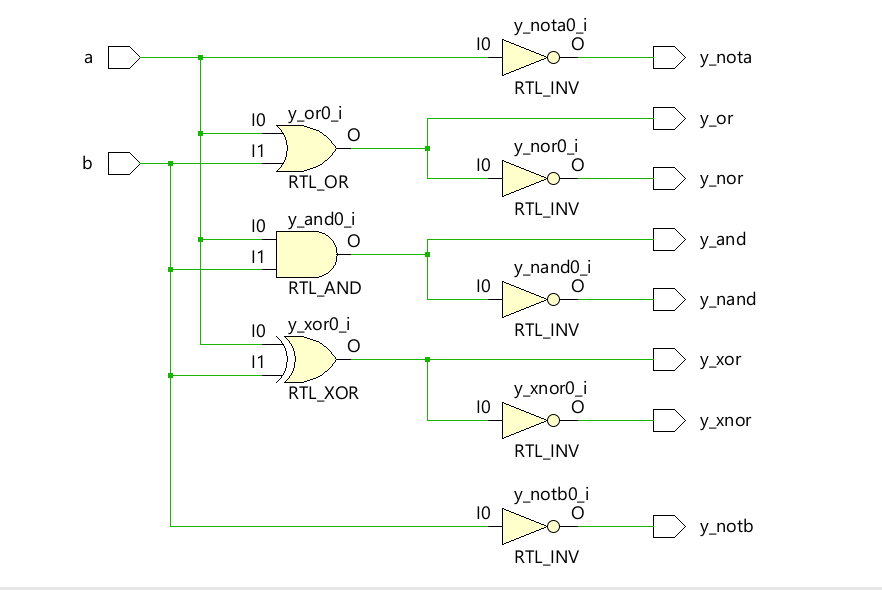
\includegraphics[width=1.0\linewidth]{images/8_rtl.png}
    \caption{Caption}
    \label{fig:placeholder}
\end{figure}


%----------------------------------------
\section{Verilog Design Code}

\begin{verilogbox}
\begin{lstlisting}
`timescale 1ns / 1ps
module exp8(
input wire a,b,
output reg y_and, y_nand, y_or, y_nor, y_xor, y_xnor, y_nota, y_notb
);

always @(*)begin
	y_and = a & b;
	y_nand = ~(a & b);
	y_or = a | b;
	y_nor = ~( a | b);
	y_xor = a ^ b;
	y_xnor = ~(a ^ b);
	y_nota = ~a;
	y_notb = ~b;
end
endmodule
\end{lstlisting}
\end{verilogbox}

%----------------------------------------
\section{Testbench Code}

\begin{verilogbox}
\begin{lstlisting}
`timescale 1ns / 1ps

module exp8_tb(

);

	reg a,b;
	wire y_or;
	exp1 uut ( a, b , y_and, y_nand, y_or, y_nor, y_xor, y_xnor, y_nota, y_notb );
	integer i;
	
	initial begin
          
          $monitor("Time = %t | a = %b | b = %b  | y_OR = %b | y_and = %b | y_nor = %b | y_nand = %b | y_XOR = %b | y_XNOR = %b ",$time,a,b,y_or,y_and,y_nor, y_nand, y_xor, y_xnor);
          for (i=0; i<4; i=i+1) 
          begin
           {a,b} = i[1:0];
           #10;
          end
          $finish;
        end
endmodule
\end{lstlisting}
\end{verilogbox}

%----------------------------------------
\section{Simulation Results}
\begin{figure}
    \centering
    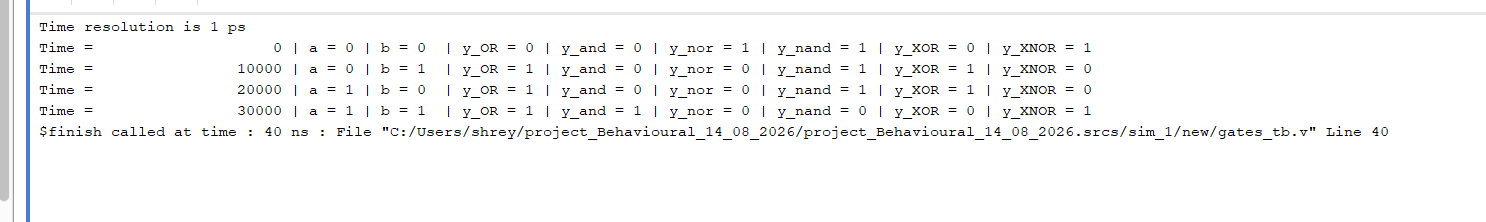
\includegraphics[width=1.0\linewidth]{images/8th_tcl.png}
     \caption{Simulation Waveform -- Realization of Logic Gates using Behavioral Modelling}
    \label{fig:placeholder}
\end{figure}


\vspace{0.5cm}

\section{Results and Observations}

The basic logic gates were successfully implemented using behavioral modeling in Verilog HDL. All possible combinations of the input signals were applied during simulation. The outputs obtained for the AND, OR, NOT, NAND, NOR, XOR, and XNOR gates were found to be consistent with their respective truth tables.

The simulation verified the correct operation of each logic gate and demonstrated the use of procedural behavioral modeling for describing combinational digital circuits.

\vspace{2cm}

\section{Conclusion}

The basic logic gates were successfully designed and implemented using behavioral modeling in Verilog HDL. The simulated outputs matched the expected truth table values for all input combinations. The experiment demonstrated how combinational logic can be described using procedural \texttt{always} blocks.

\vspace{1.5cm}

\section{Sources of Error}

\begin{itemize}
    \item Incorrect implementation of Boolean expressions may result in incorrect output values.
    \item An improper sensitivity list in the \texttt{always} block may cause simulation mismatches.
    \item Uninitialized input signals may produce unknown (\texttt{X}) values during simulation.
    \item Errors in the testbench input sequence may lead to incorrect interpretation of the results.
    \item Incorrect signal declarations or module connections may result in compilation or simulation errors.
\end{itemize}

\vspace{2.5cm}
%----------------------------------------
\chapter{Mixed Dataflow and Procedural Modeling}
\label{ch:pdf9}

\section{Objective}

To design and implement a digital circuit using both continuous assignment statements and procedural \texttt{always} blocks in Verilog HDL, and verify its functionality through simulation.

\section{Theory}

In Verilog HDL, combinational circuits can be implemented using continuous assignments and procedural blocks.

Continuous assignments use the \texttt{assign} keyword and continuously evaluate the assigned expression whenever an input changes. Procedural combinational logic can be implemented using an \texttt{always @(*)} block.

In this experiment, the following outputs are implemented:

\[
Y_1 = A + B
\]

\[
Y_2 = Y_1 \oplus C
\]

\[
Y_3 = A \cdot B
\]

\[
Y_4 = Y_3 + C
\]

\[
Y_5 = A - B
\]

The first two outputs are implemented using continuous assignment statements, while the remaining outputs are implemented using procedural \texttt{always} blocks. Both types of assignments operate concurrently.


\section{Software Tools}

Xilinx Vivado 2025.1 (Design Entry, RTL Analysis and Simulation)

\section{Procedure}

\begin{enumerate}
    \item Create a new RTL project in Vivado.
    \item Write the Verilog module with inputs $A$, $B$, and $C$ and outputs $Y_1$ to $Y_5$.
    \item Implement $Y_1$ and $Y_2$ using continuous assignment statements.
    \item Implement $Y_3$, $Y_4$, and $Y_5$ using procedural \texttt{always @(*)} blocks.
    \item Run RTL Analysis and generate the RTL schematic.
    \item Write a testbench to apply all possible input combinations.
    \item Run the behavioral simulation and view the waveform in GTKWave.
    \item Verify the outputs against the expected results.
\end{enumerate}

%----------------------------------------
\section{RTL Diagram}

\begin{figure}
    \centering
    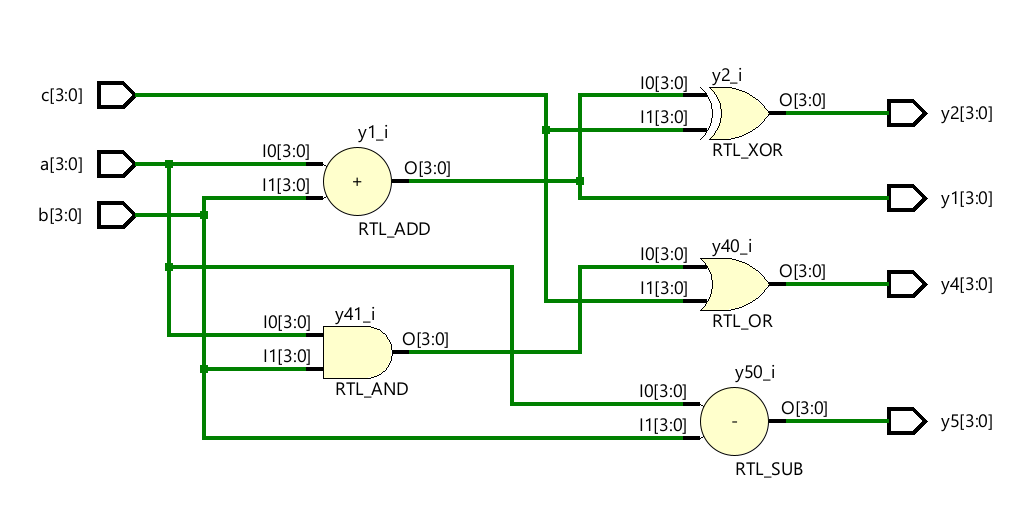
\includegraphics[width=1.0\linewidth]{images/9_rtl.png}
     \caption{RTL Schematic -- Mixed Dataflow and Procedural Modeling}
    \label{fig:placeholder}
\end{figure}

%----------------------------------------
\section{Verilog Design Code}

\begin{verilogbox}
\begin{lstlisting}
`timescale 1ns / 1ps


module bool(
input wire [3:0] a,b,c,
output wire[3:0] y1,y2,
output reg[3:0] y4,y5
    );
    
 assign y2 = y1 ^ c;
 assign y1 = a + b ;
 reg[3:0] y3;
 always @(*) begin
    y4 = y3 | c;
    y3 = a & b ;
    y5 = a - b;
    end
endmodule
 
 
\end{lstlisting}
\end{verilogbox}

%----------------------------------------
\section{Testbench Code}

\begin{verilogbox}
\begin{lstlisting}
`timescale 1ns / 1ps

module bools_tb(

    );
    
  reg [3:0] a,b,c;
  wire[3:0] y1,y2,y4,y5;
  bool uut (a,b,c,y1,y2,y4,y5);
  initial begin 
        $monitor("Time = %t | a=%b | b= %b |c=%b | y1 = %b | y2= %b | y4 = %b |y5= %b ",$time,a,b,c,y1,y2,y4,y5);
        a=4'd5; b=4'd3; c= 4'd2;
        #10;
        a=4'd10; b=4'd10; c= 4'd10;
        #10;
        a=4'd4; b=4'd8; c= 4'd0;
        #10;
        a=4'd0; b=4'd0; c= 4'd0;
        #10;
        end    
endmodule

\end{lstlisting}
\end{verilogbox}

%----------------------------------------
\section{Simulation Results}
\begin{figure}
    \centering
    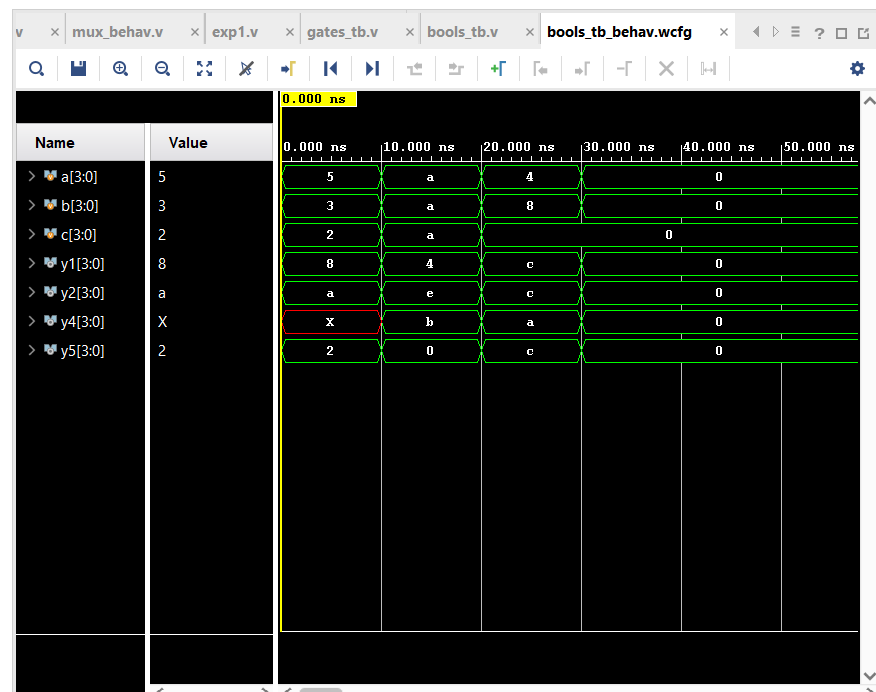
\includegraphics[width=1\linewidth]{images/9_tb.png}
    \caption{Simulation Waveform -- Mixed Dataflow and Procedural Modeling}
    \label{fig:placeholder}
\end{figure}

\begin{figure}
    \centering
    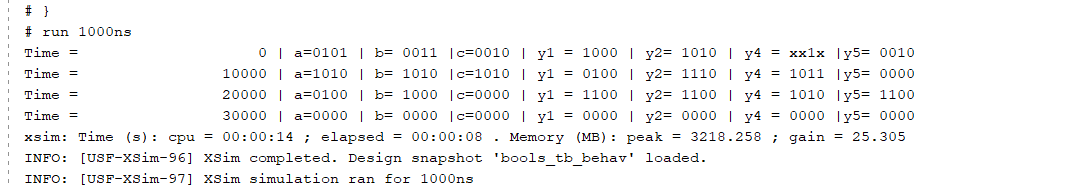
\includegraphics[width=1\linewidth]{images/9_tcl.png}
    \caption{Truth table in the TCL console}
    \label{fig:placeholder}
\end{figure}
\vspace{0.5cm}

\section{Results and Observations}

It is observed that $Y_4$ may initially show an \texttt{X} (unknown) value during simulation. This occurs because $Y_4$ depends on $Y_3$, while $Y_3$ is assigned inside a procedural \texttt{always} block. Although continuous assignments and procedural blocks operate concurrently, the updates to signals may occur in different simulation delta cycles.

When the input values change, $Y_4$ may be evaluated before the updated value of $Y_3$ is propagated. Consequently, $Y_4$ can temporarily retain an unknown value. In the subsequent delta cycle, after $Y_3$ is updated, $Y_4$ is re-evaluated and obtains its correct value.

Thus, the observed \texttt{X} is a simulation scheduling effect and does not represent a physical clock-cycle delay.

\section{Conclusion}

The circuit was successfully implemented using both continuous assignment statements and procedural \texttt{always} blocks. The simulation demonstrated the concurrent operation of these two modeling styles. The transient \texttt{X} observed at $Y_4$ illustrates the effect of Verilog simulation scheduling and delta-cycle propagation when a continuous assignment depends on a signal updated procedurally.

\section{Sources of Error}

\begin{itemize}
    \item Incorrect understanding of Verilog's event scheduling and delta-cycle behavior may lead to misinterpretation of transient \texttt{X} values.
    \item Improper sensitivity lists in procedural blocks can result in incorrect simulation behavior.
    \item Uninitialized signals may initially take an unknown (\texttt{X}) value.
    \item Incorrect ordering or dependency between intermediate signals may cause temporary unknown values during simulation.
    \item Errors in the testbench timing may affect the observation and interpretation of the waveform.
\end{itemize}

\vspace{2.5cm}

%----------------------------------------
%----------------------------------------
\chapter{Implementation of a 2-to-1 Multiplexer Using Behavioral Modeling}
\label{ch:pdf10}

\section{Objective}

To design and implement a \textbf{2-to-1 Multiplexer} using behavioral modeling in Verilog HDL using three different approaches:
\begin{enumerate}
    \item Basic behavioral implementation
    \item Implementation using \texttt{if-else} statements
    \item Implementation using \texttt{case} (switch) statements
\end{enumerate}

The functionality of all three implementations is verified through simulation.

\section{Theory}

A 2-to-1 multiplexer is a combinational circuit that selects one of two input signals and transfers the selected input to a single output based on a select line.

The multiplexer consists of two data inputs $I_0$ and $I_1$, one select input $S$, and one output $Y$.

The Boolean expression for a 2-to-1 multiplexer is:

\[
Y = \overline{S}I_0 + SI_1
\]

When $S=0$, the output follows $I_0$, while when $S=1$, the output follows $I_1$.

In behavioral modeling, the functionality of the circuit is described using procedural constructs inside an \texttt{always} block rather than explicitly specifying individual logic gates.

The three approaches used in this experiment demonstrate different ways of describing the same multiplexer functionality.

\section{Truth Table}

\begin{table}[H]
    \centering
    \caption{Truth Table of 2-to-1 Multiplexer}
    \label{tab:mux2_behavioral}
    \begin{tabular}{|c|c|c|}
    \hline
    \textbf{$S$} & \textbf{Selected Input} & \textbf{Output $Y$} \\
    \hline
    0 & $I_0$ & $I_0$ \\
    \hline
    1 & $I_1$ & $I_1$ \\
    \hline
    \end{tabular}
\end{table}

\section{Software Tools}

Xilinx Vivado 2025.1 (Design Entry, RTL Analysis and Simulation)

\section{Procedure}

\begin{enumerate}
    \item Create a new RTL project in Vivado.
    \item Define two data inputs $I_0$ and $I_1$, one select input $S$, and output $Y$.
    \item Implement the 2-to-1 multiplexer using basic behavioral modeling.
    \item Implement the same multiplexer using an \texttt{if-else} statement.
    \item Implement the same multiplexer using a \texttt{case} statement.
    \item Run RTL Analysis and generate the RTL schematic.
    \item Write a testbench to apply all possible combinations of the input and select signals.
    \item Run the behavioral simulation.
    \item Compare the outputs of all three implementations.
    \item Verify the results against the expected truth table.
\end{enumerate}

%----------------------------------------
\section{RTL Diagram}

\begin{figure}[H]
    \centering
    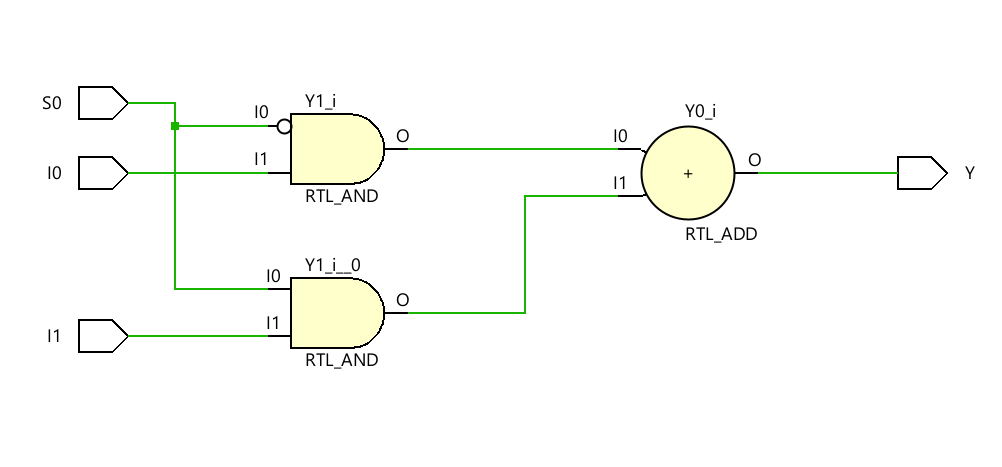
\includegraphics[width=0.9\textwidth]{images/10_rtl.png}
    \caption{RTL Schematic -- 2-to-1 Multiplexer Using Behavioral Modeling}
    \label{fig:10_rtl}
\end{figure}

%----------------------------------------
\section{Verilog Design Code}

\subsection{Part 1: Basic Behavioral Implementation}

\begin{verilogbox}
\begin{lstlisting}
module mux2_b(
input wire I0,
input wire I1,
input wire S0,
output reg Y

);

always @(*) begin
    Y = (~S0 & I0) + ( S0 & I1);
    end 
endmodule
\end{lstlisting}
\end{verilogbox}

\subsection{Part 2: Implementation Using If-Else Statements}

\begin{verilogbox}
\begin{lstlisting}

module mux_behav(
input wire IO,I1,S0,
output reg Y
    );
    
    always @(*) begin
        if (S0 == 1'b0) begin
            Y=IO;
        end else begin
            Y=I1;
        end 
    end
       
endmodule

\end{lstlisting}
\end{verilogbox}

\subsection{Part 3: Implementation Using Case Statements}

\begin{verilogbox}
\begin{lstlisting}

module mux_case(
input wire I0,I1,S0,
output reg Y
    );
    
  always @(*) begin
     case(S0)
       1'b0:Y=I0;
       1'b1:Y=I1;
       default Y=1'b0;
     endcase
     end
endmodule

\end{lstlisting}
\end{verilogbox}

%----------------------------------------
\section{Testbench Code}

\begin{verilogbox}
\begin{lstlisting}

module muxtwox1_tb(

    );


 reg IO,I1,S0;
 wire Y;

mux_behav uut ( .IO(IO),
.I1(I1), . S0(S0) , .Y( Y) );

integer i;
initial begin
    $monitor( "Time = %b  |  S0 = %b  |  I0 = %b   |  I1 = %b | Y= %b " , $time , S0, IO, I1  , Y );
    
    for (i=0;i<4;i=i+1) begin
        {I1,IO,S0}=i[2:0];
            #1;
            end
        $finish;
        end 

endmodule
\end{lstlisting}
\end{verilogbox}

%----------------------------------------
\section{Simulation Results}

\begin{figure}[H]
    \centering
    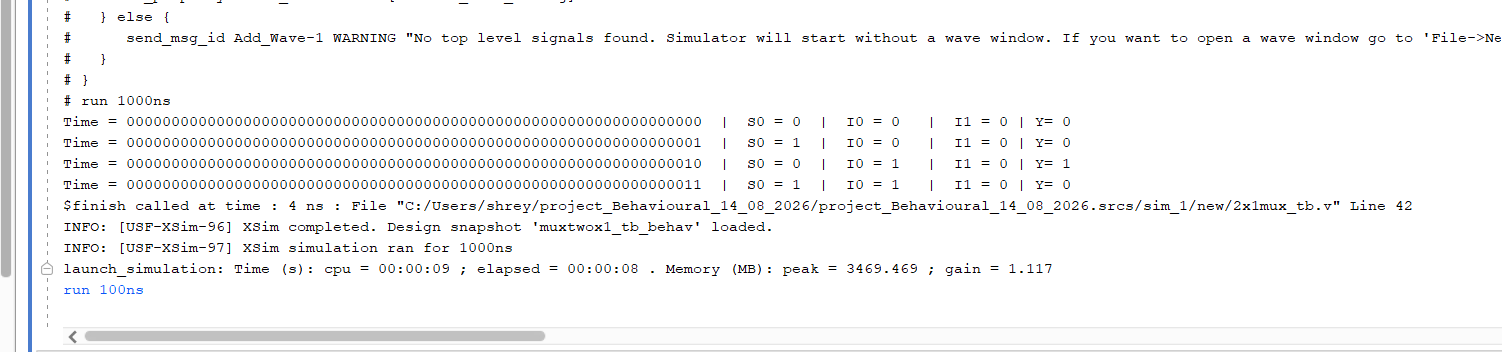
\includegraphics[width=1.5\textwidth]{images/10_tcl.png}
    \caption{Truth table verification  -- 2-to-1 Multiplexer Using Behavioral Modeling}
    \label{fig:10_wave}
\end{figure}

\vspace{0.5cm}

\section{Results and Observations}

The 2-to-1 multiplexer was successfully implemented using three different behavioral modeling approaches. The first implementation used a basic behavioral description, the second implementation used an \texttt{if-else} statement, and the third implementation used a \texttt{case} statement.

For all possible combinations of the select and input signals, the outputs of all three implementations were observed to be identical.

When $S=0$, the output was equal to $I_0$, whereas when $S=1$, the output was equal to $I_1$. The simulation results were consistent with the expected truth table.

\vspace{2cm}

\section{Conclusion}

A 2-to-1 multiplexer was successfully designed and implemented using behavioral modeling in Verilog HDL. Three different approaches, namely basic behavioral modeling, \texttt{if-else}, and \texttt{case} statements, were used to describe the same combinational functionality. The simulation results verified the correct operation of all three implementations.

\vspace{1.5cm}

\section{Sources of Error}

\begin{itemize}
    \item Incorrect implementation of the select condition may cause the wrong input to appear at the output.
    \item Missing or incorrect sensitivity in the behavioral block may result in improper simulation behavior.
    \item Incorrect \texttt{if-else} conditions may cause incorrect input selection.
    \item Incorrect \texttt{case} conditions or missing cases may result in unexpected or unknown outputs.
    \item Uninitialized input signals may produce unknown (\texttt{X}) values during simulation.
    \item Errors in the testbench input sequence may result in incomplete verification.
\end{itemize}

\vspace{2.5cm}
%----------------------------------------
%----------------------------------------
\chapter{Implementation of a 4-to-1 Multiplexer Using Behavioral Modeling}
\label{ch:pdf21}

\section{Objective}

To design and implement a \textbf{4-to-1 multiplexer} using behavioral modeling in Verilog HDL through three different approaches: basic behavioral implementation, if-else statements, and case statements, and to verify their functionality through simulation.

\section{Theory}

A multiplexer (MUX) is a combinational digital circuit that selects one of several input signals and transfers the selected input to a single output.

A 4-to-1 multiplexer has four data inputs $I_0$, $I_1$, $I_2$, and $I_3$, two select inputs $S_1$ and $S_0$, and one output $Y$.

The selected input is determined by the select lines according to

\[
Y =
\begin{cases}
I_0, & S_1S_0 = 00 \\
I_1, & S_1S_0 = 01 \\
I_2, & S_1S_0 = 10 \\
I_3, & S_1S_0 = 11
\end{cases}
\]

The Boolean expression for the 4-to-1 multiplexer is

\[
Y = \overline{S_1}\overline{S_0}I_0
+ \overline{S_1}S_0I_1
+ S_1\overline{S_0}I_2
+ S_1S_0I_3.
\]

In behavioral modeling, the operation of the multiplexer is described using procedural constructs rather than explicitly instantiating logic gates.

Three behavioral approaches are implemented:

\begin{enumerate}
    \item \textbf{Part 1 -- Basic Behavioral Implementation:} Uses a conditional expression to select the required input.
    \item \textbf{Part 2 -- If-Else Implementation:} Uses nested \texttt{if-else} statements to implement the selection logic.
    \item \textbf{Part 3 -- Case Implementation:} Uses a \texttt{case} statement based on the two select inputs.
\end{enumerate}

\section{Truth Table}

\begin{table}[H]
    \centering
    \begin{tabular}{|c|c|c|c|c|c|}
        \hline
        \textbf{$S_1$} & \textbf{$S_0$} & \textbf{$I_0$} & \textbf{$I_1$} & \textbf{$I_2$} & \textbf{$I_3$} \\
        \hline
        0 & 0 & X & X & X & X \\
        \hline
        0 & 1 & X & X & X & X \\
        \hline
        1 & 0 & X & X & X & X \\
        \hline
        1 & 1 & X & X & X & X \\
        \hline
    \end{tabular}
    \qquad
    \begin{tabular}{|c|c|}
        \hline
        \textbf{Select} & \textbf{Output} \\
        \hline
        00 & $I_0$ \\
        \hline
        01 & $I_1$ \\
        \hline
        10 & $I_2$ \\
        \hline
        11 & $I_3$ \\
        \hline
    \end{tabular}
    \caption{Truth table of a 4-to-1 multiplexer}
    \label{tab:4to1_mux_behavioral}
\end{table}

\section{Software Tools}

Xilinx Vivado 2025.1 (Design Entry, RTL Analysis and Simulation)

\section{Procedure}

\begin{enumerate}
    \item Create a new RTL project in Xilinx Vivado.
    
    \item Define the four data inputs, two select inputs, and output of the 4-to-1 multiplexer.
    
    \item Implement the multiplexer using basic behavioral modeling.
    
    \item Implement the same multiplexer using nested if-else statements.
    
    \item Implement the same multiplexer using a case statement.
    
    \item Run RTL Analysis and generate the RTL schematic for the designs.
    
    \item Write a testbench to apply different combinations of select and data inputs.
    
    \item Run behavioral simulation and observe the output waveform.
    
    \item Verify that the selected input appears at the output for every combination of the select lines.
\end{enumerate}

%----------------------------------------
\section{RTL Diagram}
\begin{figure}[H]
    \centering
    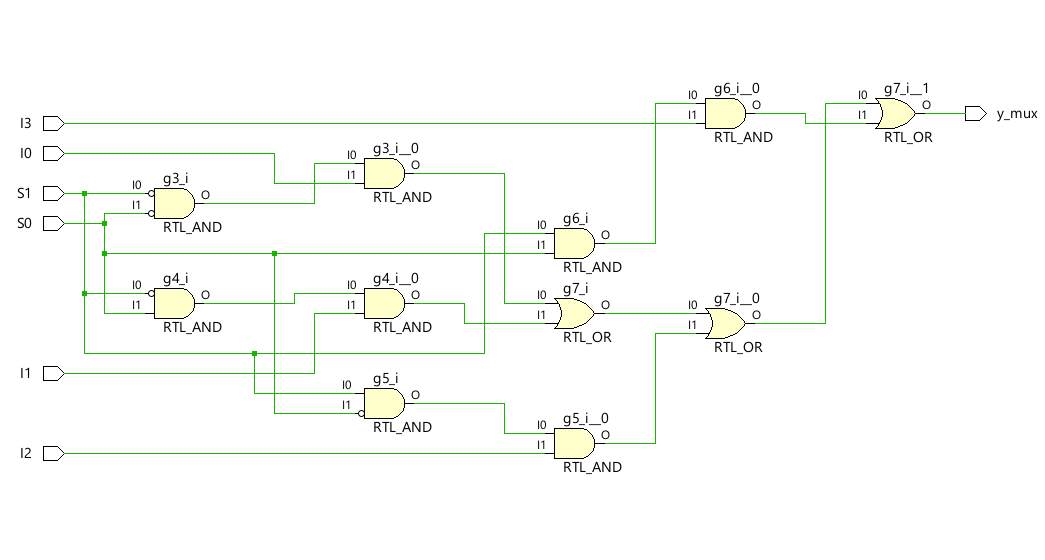
\includegraphics[width=0.9\textwidth]{images/6_rtl}
    \caption{RTL Schematic -- 4-to-1 Multiplexer Using Structural Modeling}
    \label{fig:6_rtl}
\end{figure}


%----------------------------------------
\section{Verilog Design Code}

\subsection{Part 1: Basic Behavioral Implementation}

\begin{verilogbox}
\begin{lstlisting}
`timescale 1ns/1ps

module mux_basic (
    input  wire I0,
    input  wire I1,
    input  wire I2,
    input  wire I3,
    input  wire S0,
    input  wire S1,
    output reg  Y
);

    always @(*) begin
        Y = (S1 == 1'b0 && S0 == 1'b0) ? I0 :
            (S1 == 1'b0 && S0 == 1'b1) ? I1 :
            (S1 == 1'b1 && S0 == 1'b0) ? I2 :
                                         I3;
    end

endmodule
\end{lstlisting}
\end{verilogbox}

\subsection{Part 2: Implementation Using If-Else Statements}

\begin{verilogbox}
\begin{lstlisting}
`timescale 1ns/1ps

module mux_ifelse (
    input  wire I0,
    input  wire I1,
    input  wire I2,
    input  wire I3,
    input  wire S0,
    input  wire S1,
    output reg  Y
);

    always @(*) begin
        if (S1 == 1'b0 && S0 == 1'b0)
            Y = I0;
        else if (S1 == 1'b0 && S0 == 1'b1)
            Y = I1;
        else if (S1 == 1'b1 && S0 == 1'b0)
            Y = I2;
        else
            Y = I3;
    end

endmodule
\end{lstlisting}
\end{verilogbox}

\subsection{Part 3: Implementation Using Case Statement}

\begin{verilogbox}
\begin{lstlisting}
`timescale 1ns/1ps

module mux_case (
    input  wire I0,
    input  wire I1,
    input  wire I2,
    input  wire I3,
    input  wire S0,
    input  wire S1,
    output reg  Y
);

    always @(*) begin
        case ({S1, S0})
            2'b00: Y = I0;
            2'b01: Y = I1;
            2'b10: Y = I2;
            2'b11: Y = I3;
            default: Y = 1'b0;
        endcase
    end

endmodule
\end{lstlisting}
\end{verilogbox}

%----------------------------------------
\section{Testbench Code}

\begin{verilogbox}
\begin{lstlisting}
`timescale 1ns/1ps

module mux_4to1_tb;

    reg I0, I1, I2, I3;
    reg S0, S1;

    wire Y_basic;
    wire Y_ifelse;
    wire Y_case;

    mux_basic uut_basic (
        .I0(I0),
        .I1(I1),
        .I2(I2),
        .I3(I3),
        .S0(S0),
        .S1(S1),
        .Y(Y_basic)
    );

    mux_ifelse uut_ifelse (
        .I0(I0),
        .I1(I1),
        .I2(I2),
        .I3(I3),
        .S0(S0),
        .S1(S1),
        .Y(Y_ifelse)
    );

    mux_case uut_case (
        .I0(I0),
        .I1(I1),
        .I2(I2),
        .I3(I3),
        .S0(S0),
        .S1(S1),
        .Y(Y_case)
    );

    integer i;

    initial begin

        $monitor("Time = %0t | S1 = %b | S0 = %b | I0 = %b | I1 = %b | I2 = %b | I3 = %b | Basic = %b | If-Else = %b | Case = %b",
                 $time, S1, S0, I0, I1, I2, I3,
                 Y_basic, Y_ifelse, Y_case);

        // Data inputs
        I0 = 1'b0;
        I1 = 1'b1;
        I2 = 1'b0;
        I3 = 1'b1;

        // Test all select combinations
        for (i = 0; i < 4; i = i + 1) begin
            {S1, S0} = i[1:0];
            #10;
        end

        // Change data inputs
        I0 = 1'b1;
        I1 = 1'b0;
        I2 = 1'b1;
        I3 = 1'b0;

        for (i = 0; i < 4; i = i + 1) begin
            {S1, S0} = i[1:0];
            #10;
        end

        $finish;
    end

endmodule
\end{lstlisting}
\end{verilogbox}

%----------------------------------------
\section{Simulation Results}

\begin{figure}[H]
    \centering
    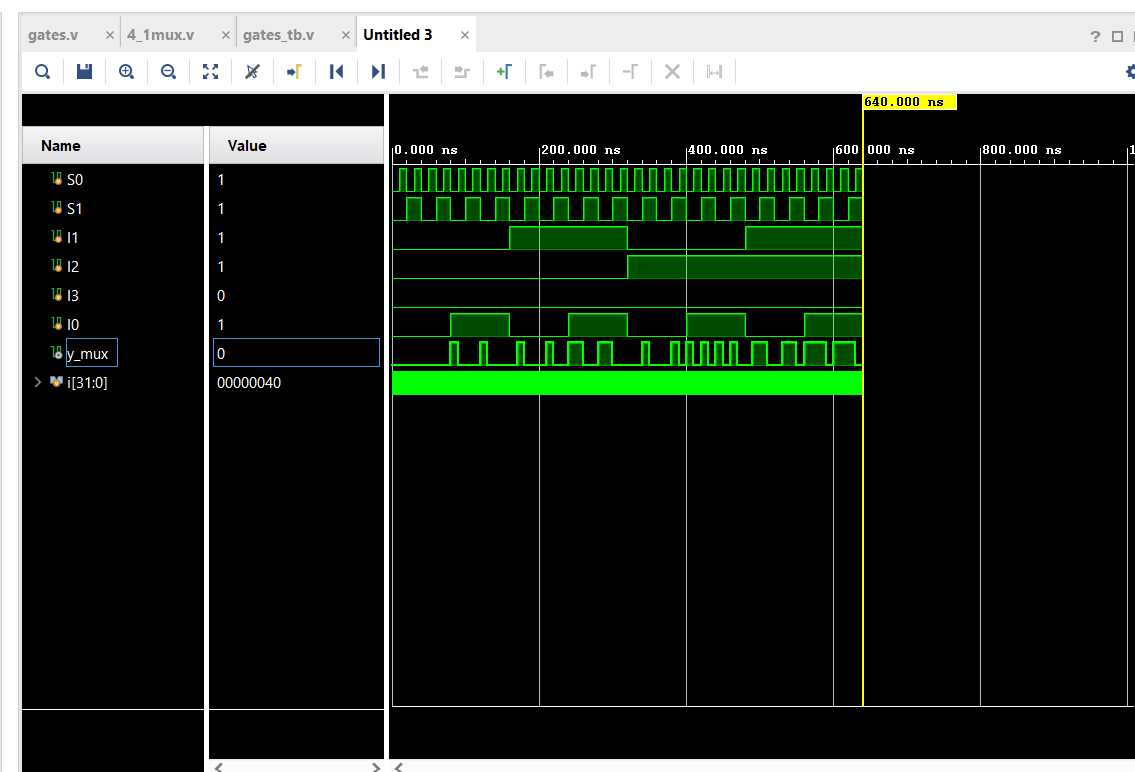
\includegraphics[width=0.95\textwidth]{images/6_wave}
    \caption{Simulation Waveform -- 4-to-1 Multiplexer Using Structural Modeling}
    \label{fig:6_wave}
\end{figure}

\vspace{0.5cm}

\section{Results and Observations}

\begin{itemize}
    \item The 4-to-1 multiplexer was successfully implemented using three behavioral modeling techniques.
    
    \item In all three implementations, the output follows the input selected by the select lines.
    
    \item For $S_1S_0=00$, the output follows $I_0$.
    
    \item For $S_1S_0=01$, the output follows $I_1$.
    
    \item For $S_1S_0=10$, the output follows $I_2$.
    
    \item For $S_1S_0=11$, the output follows $I_3$.
    
    \item The simulation results of the basic behavioral, if-else, and case implementations are identical for the applied test cases.
\end{itemize}

\section{Conclusion}

A 4-to-1 multiplexer was successfully designed using behavioral modeling in Verilog HDL. Three different behavioral approaches, namely conditional expression, if-else statements, and case statements, were implemented and verified. All three implementations produced the expected output for the applied combinations of select and data inputs.

\section{Sources of Error}

\begin{itemize}
    \item Incorrect mapping of select inputs to the corresponding data inputs can result in an incorrect output.
    
    \item Missing or incorrect sensitivity in a combinational procedural block can lead to simulation mismatches.
    
    \item Failure to assign the output for all possible select conditions may result in inferred latches.
    
    \item Incorrect testbench input combinations may result in incomplete verification.
\end{itemize}

%-----------------------------------------
%----------------------------------------
\chapter{Realization of 3:8 Decoder}
\label{ch:exp6}

\section{Objective}

To design and verify a \textbf{3:8 Decoder} using Verilog HDL and validate its functionality through RTL analysis and simulation.

\section{Theory}

A \textbf{3:8 Decoder} is a combinational logic circuit that converts a three-bit binary input into one of eight unique output lines. The three input lines, represented as $S_2$, $S_1$, and $S_0$, determine which output line is activated.

The decoder has eight outputs, denoted by $Y_0$ to $Y_7$. For every valid combination of the three input bits, only one output is active at a time. This type of output is commonly referred to as a \textbf{one-hot output}.

For an active-high decoder with an enable input $E$, the decoder operates when $E = 1$. When the decoder is disabled ($E = 0$), all outputs remain LOW.

The Boolean expressions for the outputs are:

\[
Y_0 = E\overline{S_2}\overline{S_1}\overline{S_0}
\]

\[
Y_1 = E\overline{S_2}\overline{S_1}S_0
\]

\[
Y_2 = E\overline{S_2}S_1\overline{S_0}
\]

\[
Y_3 = E\overline{S_2}S_1S_0
\]

\[
Y_4 = ES_2\overline{S_1}\overline{S_0}
\]

\[
Y_5 = ES_2\overline{S_1}S_0
\]

\[
Y_6 = ES_2S_1\overline{S_0}
\]

\[
Y_7 = ES_2S_1S_0
\]

\section{Truth Table}

\begin{table}[H]
    \centering
    \caption{Truth Table -- 3:8 Decoder}
    \begin{tabular}{|c|c|c|}
        \hline
        \textbf{Enable ($E$)} & \textbf{Select ($S_2S_1S_0$)} & \textbf{Output ($Y_7Y_6Y_5Y_4Y_3Y_2Y_1Y_0$)} \\
        \hline
        0 & XXX & 00000000 \\
        \hline
        1 & 000 & 00000001 \\
        1 & 001 & 00000010 \\
        1 & 010 & 00000100 \\
        1 & 011 & 00001000 \\
        1 & 100 & 00010000 \\
        1 & 101 & 00100000 \\
        1 & 110 & 01000000 \\
        1 & 111 & 10000000 \\
        \hline
    \end{tabular}
\end{table}

\vspace{0.5cm}

\section{Software Tools}

Xilinx Vivado 2025.1 (Design Entry, RTL Analysis and Simulation), GTKWave (Waveform Viewer)

\section{Procedure}

\begin{enumerate}
    \item Create a new RTL project in Vivado.
    
    \item Create a Verilog source file and write the design module for the 3:8 Decoder.
    
    \item Define the three-bit select input, enable input, and eight-bit output.
    
    \item Implement the decoding operation using a suitable Verilog modeling style.
    
    \item Run RTL Analysis and generate the RTL schematic of the design.
    
    \item Write a Verilog testbench to apply all eight possible combinations of the select inputs.
    
    \item Enable the decoder and verify the corresponding one-hot output for each select combination.
    
    \item Disable the decoder and verify that all output lines become LOW.
    
    \item Run the behavioral simulation and observe the output waveform.
    
    \item Verify the simulation results using the expected truth table.
\end{enumerate}

%----------------------------------------
\section{RTL Diagram}
\begin{figure}
    \centering
    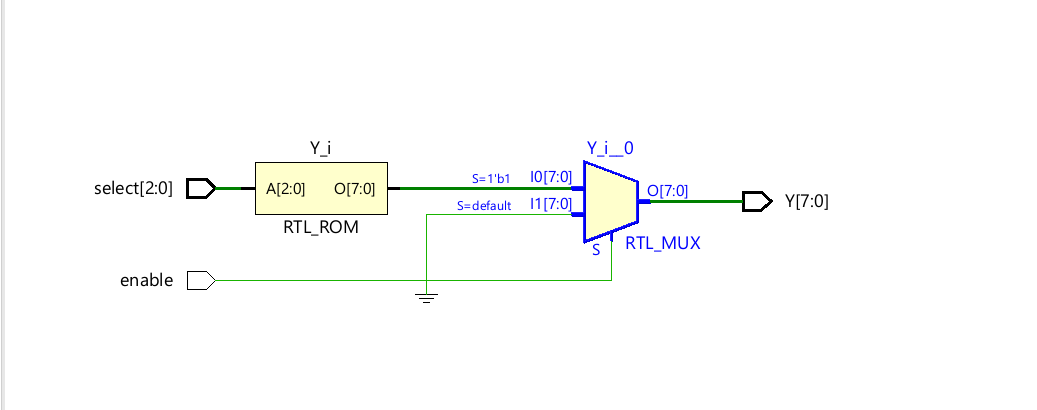
\includegraphics[width=1.0\linewidth]{3_8_decoder.png}
 \caption{RTL Schematic of 3:8 Decoder}    \label{fig:placeholder}
\end{figure}

%----------------------------------------
\section{Verilog Design Code}

\begin{verilogbox}
\begin{lstlisting}
module decoder(
    input wire [2:0] select,
    input wire enable,
    output reg [7:0] Y
);

always @(*) begin
    if (enable == 1'b1) begin
        case(select)
            3'b000: Y = 8'b00000001;
            3'b001: Y = 8'b00000010;
            3'b010: Y = 8'b00000100;
            3'b011: Y = 8'b00001000;
            3'b100: Y = 8'b00010000;
            3'b101: Y = 8'b00100000;
            3'b110: Y = 8'b01000000;
            3'b111: Y = 8'b10000000;
            default: Y = 8'b00000000;
        endcase
    end
    else begin
        Y = 8'b00000000;
    end
end

endmodule
\end{lstlisting}
\end{verilogbox}

%----------------------------------------
\section{Testbench Code}

\begin{verilogbox}
\begin{lstlisting}
`timescale 1ns / 1ps


module decoder_tb(



    );
    
    reg [2:0] select;
    reg enable;
    wire [7:0] Y;
    decoder uut ( select,enable,Y);
    integer i;
    initial begin
            $monitor("Time = %t | select = %b | enable = %b | Y = %b", $time, select, enable, Y );
            // Enable the decoder
            
            enable = 1'b1;
            
            for (i=0;i<8;i=i+1) begin
           {select}=i[2:0];
            #10;
            end
            
            //enable = 1'b0;
            //for (i=8;i<15;i=i+1) begin
           //{select}=i[2:0];
            //#10;
            //end
            
        $finish;
        
        
        end 
    
endmodule





\end{lstlisting}
\end{verilogbox}

%----------------------------------------
\section{Simulation Results}
\begin{figure}
    \centering
    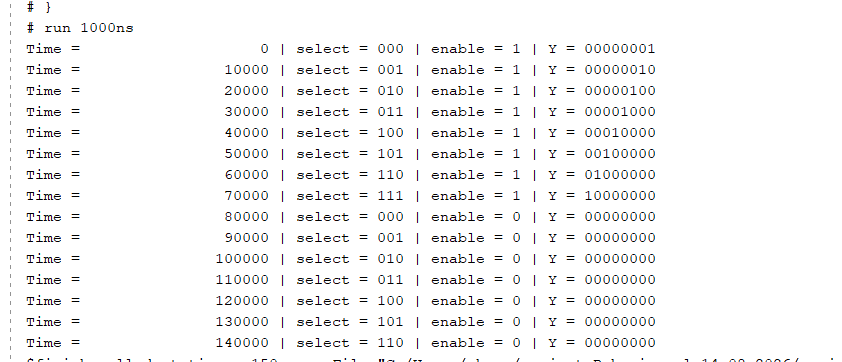
\includegraphics[width=1.0\linewidth]{3_8_tcl.png}
\caption{Truth Table Verification - 3:8 Decoder}    \label{fig:placeholder}
\end{figure}

\vspace{0.5cm}

\section{Results and Observations}

The 3:8 Decoder was successfully designed and simulated using Verilog HDL. When the enable input was HIGH, each combination of the three-bit select input activated the corresponding output line while keeping all other outputs LOW.

For example:

\[
S_2S_1S_0 = 000 \Rightarrow Y = 00000001
\]

\[
S_2S_1S_0 = 001 \Rightarrow Y = 00000010
\]

\[
S_2S_1S_0 = 010 \Rightarrow Y = 00000100
\]

and similarly for all remaining input combinations.

When the enable input was LOW, all output lines were observed to be LOW, confirming the correct operation of the enable functionality.

\vspace{0.5cm}

\section{Conclusion}

The 3:8 Decoder was successfully realized using Verilog HDL and verified through simulation. The circuit correctly decoded each of the eight possible combinations of the three-bit select input into a unique active output line. The enable input was also verified successfully, with all outputs becoming LOW when the decoder was disabled. The simulation results were found to be consistent with the expected truth table.

\section{Sources of Error}

\begin{itemize}
    \item Incorrect assignment of output values in the Verilog code.
    \item Incorrect ordering of the select input bits.
    \item Failure to initialize input signals in the testbench.
    \item Incorrect implementation of the enable logic.
    \item Insufficient simulation time for observing all input combinations.
    \item Errors in interpreting the output bit order during waveform analysis.
\end{itemize}
%----------------------------------------
\chapter{Multiplication and Division Using Shift Operations}
\label{ch:pdf13}

\section{Objective}

To implement basic arithmetic operations using shift operations in Verilog HDL, specifically:
\begin{enumerate}
    \item Multiplication using the left-shift operation.
    \item Division using the right-shift operation.
\end{enumerate}

The functionality of the implemented circuits is verified through simulation.

\section{Theory}

Shift operations are commonly used in digital systems to perform efficient arithmetic operations involving powers of two.

A left shift by one position is equivalent to multiplying an unsigned binary number by 2:

\[
A \times 2 = A << 1
\]

Similarly, a right shift by one position is equivalent to dividing an unsigned binary number by 2, with the fractional portion discarded:

\[
A \div 2 = A >> 1
\]

More generally:

\[
A \times 2^n = A << n
\]

\[
A \div 2^n = A >> n
\]

In Verilog HDL, the left-shift operator is represented by \texttt{<<}, while the right-shift operator is represented by \texttt{>>}.

For this experiment, multiplication and division by 2 are implemented using one-bit left and right shifts respectively.

\section{Software Tools}

Xilinx Vivado 2025.1 (Design Entry, RTL Analysis and Simulation)

\section{Procedure}

\begin{enumerate}
    \item Create a new RTL project in Vivado.
    \item Define an unsigned binary input of suitable width.
    \item Implement multiplication by 2 using a left-shift operation.
    \item Implement division by 2 using a right-shift operation.
    \item Write a testbench to apply different binary input values.
    \item Run RTL Analysis and generate the RTL schematic.
    \item Run the behavioral simulation.
    \item Observe the multiplication and division outputs.
    \item Compare the simulated results with the expected arithmetic values.
\end{enumerate}

%----------------------------------------
\section{RTL Diagram}

\begin{figure}[H]
    \centering
    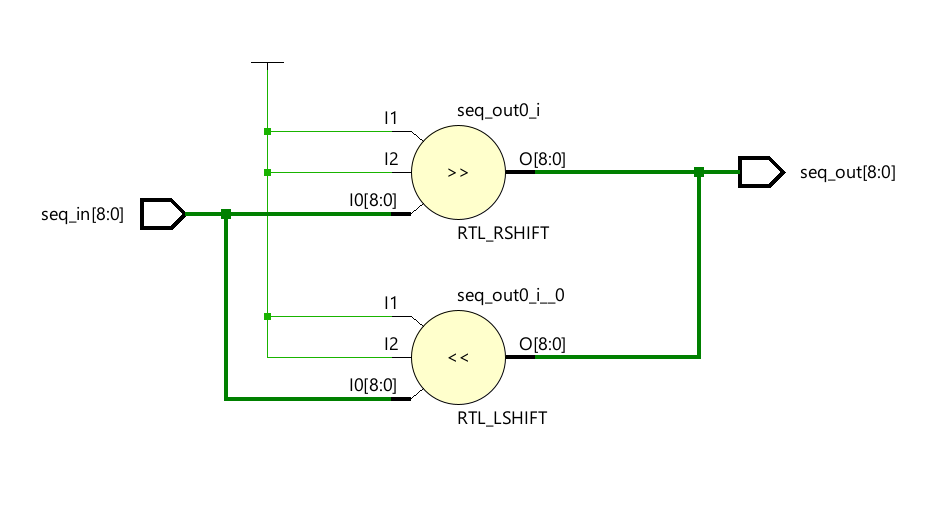
\includegraphics[width=0.9\textwidth]{images/13_rtl.png}
    \caption{RTL Schematic -- Multiplication and Division Using Shift Operations}
    \label{fig:13_rtl}
\end{figure}

%----------------------------------------
\section{Verilog Design Code}

\begin{verilogbox}
\begin{lstlisting}


module exp13(
input wire [8:0] seq_in,
output reg [8:0] seq_out

    );
    
 always @(*) begin
     seq_out = seq_in << 1;
     end
     
 always @(*) begin 
    seq_out = seq_in >> 1;
    end
     
endmodule

\end{lstlisting}
\end{verilogbox}

%----------------------------------------
\section{Testbench Code}

\begin{verilogbox}
\begin{lstlisting}
`timescale 1ns / 1ps


module exp13_tb(

    );
    
      reg  [8:0] seq_in;
      wire [8:0] seq_out;

    exp13 uut (
        .seq_in(seq_in),
        .seq_out(seq_out)
    );

    initial begin

        $monitor("Time = %0t | Input = %b (%0d) | Output = %b (%0d)",
                 $time, seq_in, seq_in, seq_out, seq_out);

        seq_in = 9'd2;
        #10;

        seq_in = 9'd4;
        #10;

        seq_in = 9'd5;
        #10;

        seq_in = 9'd8;
        #10;

        seq_in = 9'd10;
        #10;

        seq_in = 9'd15;
        #10;

        $finish;

    end

endmodule
\end{lstlisting}
\end{verilogbox}

%----------------------------------------
\section{Simulation Results}

\begin{figure}[H]
    \centering
    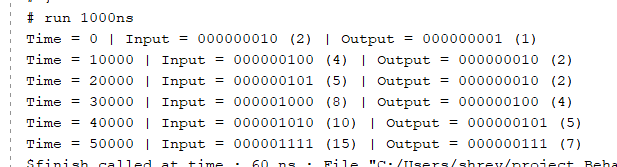
\includegraphics[width=1.2\textwidth]{images/13_sim.png}
    \caption{TCL Waveform -- Multiplication and Division Using Shift Operations}
    \label{fig:13_wave}
\end{figure}

\vspace{0.5cm}

\section{Results and Observations}

The multiplication and division operations were successfully implemented using shift operations in Verilog HDL.

The left-shift operation produced an output equivalent to multiplying the input by 2, while the right-shift operation produced an output equivalent to dividing the input by 2 for unsigned inputs.

The simulation results were consistent with the expected arithmetic results. It was also observed that right-shift division discards any fractional portion of the result.


\section{Conclusion}

Multiplication and division by powers of two were successfully implemented using shift operations in Verilog HDL. The experiment demonstrated that a left shift can be used for efficient multiplication by powers of two, while a right shift can be used for division by powers of two in unsigned binary arithmetic.



\section{Sources of Error}

\begin{itemize}
    \item Incorrect shift direction may result in an incorrect arithmetic operation.
    \item Insufficient bit width may cause overflow during left-shift operations.
    \item Right-shift operations may discard fractional portions of the result.
    \item Incorrect interpretation of signed and unsigned data may produce unexpected results.
    \item Uninitialized input signals may produce unknown (\texttt{X}) values during simulation.
    \item Errors in the testbench input values may result in incomplete verification.
\end{itemize}


%------------------------------------------

%----------------------------------------
\chapter{Implementation of a Decoder Using Shift Operations}
\label{ch:pdf14}

\section{Objective}

To design and implement a \textbf{2-to-4 Decoder} using the left-shift operation in Verilog HDL and verify its functionality through simulation.

\section{Theory}

A decoder is a combinational circuit that converts an $n$-bit binary input into one of $2^n$ possible output lines. For a 2-to-4 decoder, two input bits are used to activate one of four output lines.

The decoder has two input signals $A_1$ and $A_0$ and four output signals $Y_3$, $Y_2$, $Y_1$, and $Y_0$.

The output corresponding to the binary value of the input is activated while all other outputs remain zero.

The decoding operation can be implemented efficiently using the left-shift operation. A constant value of 1 is shifted left by the number represented by the input:

\[
Y = 1 << A
\]

where $A$ represents the binary input.

For a 2-bit input, the operation produces a 4-bit one-hot output. Thus:

\[
00 \rightarrow 0001
\]

\[
01 \rightarrow 0010
\]

\[
10 \rightarrow 0100
\]

\[
11 \rightarrow 1000
\]

The left-shift operation therefore directly generates the required decoded output without explicitly using individual logic gates.

\section{Truth Table}

\begin{table}[H]
    \centering
    \caption{Truth Table of 2-to-4 Decoder}
    \label{tab:decoder_shift}
    \begin{tabular}{|c|c|c|c|c|}
    \hline
    \textbf{$A_1$} & \textbf{$A_0$} & \textbf{$Y_3$} &
    \textbf{$Y_2$} & \textbf{$Y_1$} & \textbf{$Y_0$} \\
    \hline
    0 & 0 & 0 & 0 & 0 & 1 \\
    \hline
    0 & 1 & 0 & 0 & 1 & 0 \\
    \hline
    1 & 0 & 0 & 1 & 0 & 0 \\
    \hline
    1 & 1 & 1 & 0 & 0 & 0 \\
    \hline
    \end{tabular}
\end{table}

\section{Software Tools}

Xilinx Vivado 2025.1 (Design Entry, RTL Analysis and Simulation)

\section{Procedure}

\begin{enumerate}
    \item Create a new RTL project in Vivado.
    \item Define a 2-bit input and a 4-bit output.
    \item Implement the decoder using the left-shift operation.
    \item Use a constant value of 1 and shift it according to the binary input.
    \item Write a testbench to apply all possible combinations of the input.
    \item Run RTL Analysis and generate the RTL schematic.
    \item Run the behavioral simulation.
    \item Observe the decoded output for each input combination.
    \item Verify the simulation results against the truth table.
\end{enumerate}

%----------------------------------------
\section{RTL Diagram}

\begin{figure}[H]
    \centering
    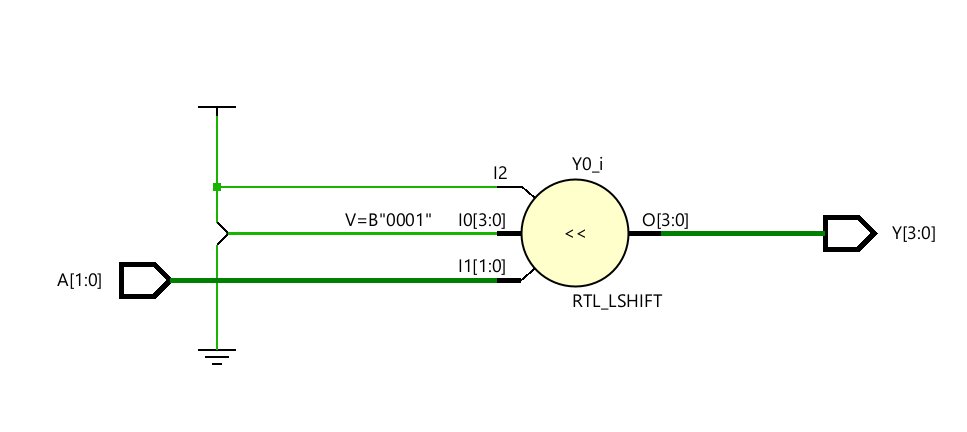
\includegraphics[width=0.9\textwidth]{images/14_rtl.png}
    \caption{RTL Schematic -- 2-to-4 Decoder Using Shift Operations}
    \label{fig:14_rtl}
\end{figure}

%----------------------------------------
\section{Verilog Design Code}

\begin{verilogbox}
\begin{lstlisting}

module decoder_shift(
    input  wire [1:0] A,
    output reg  [3:0] Y
);

    always @(*) begin
        Y = 4'b0001 << A;
    end

endmodule
\end{lstlisting}
\end{verilogbox}

%----------------------------------------
\section{Testbench Code}

\begin{verilogbox}
\begin{lstlisting}

`timescale 1ns/1ps

module decoder_shift_tb(

);

    reg  [1:0] A;
    wire [3:0] Y;

    decoder_shift uut (
        .A(A),
        .Y(Y)
    );

    integer i;

    initial begin

        $monitor("Time = %0t | A = %b | Y = %b",
                 $time, A, Y);

        for (i = 0; i < 4; i = i + 1) begin
            A = i[1:0];
            #10;
        end

        $finish;

    end

endmodule
\end{lstlisting}
\end{verilogbox}

%----------------------------------------
\section{Simulation Results}

\begin{figure}[H]
    \centering
    \includegraphics[width=0.95\textwidth]{images/14_wave}
    \caption{Simulation Waveform -- 2-to-4 Decoder Using Shift Operations}
    \label{fig:14_wave}
\end{figure}


\section{Results and Observations}

The 2-to-4 decoder was successfully implemented using the left-shift operation in Verilog HDL.

It was observed that the left-shift operation activates exactly one output bit corresponding to the binary value of the input. For an input of $00$, $01$, $10$, and $11$, the outputs obtained were $0001$, $0010$, $0100$, and $1000$, respectively.

The simulation results were consistent with the expected truth table, confirming the correct operation of the decoder.


\section{Conclusion}

A 2-to-4 decoder was successfully designed and implemented using the left-shift operation in Verilog HDL. The experiment demonstrated that a simple shift operation can be used to generate a one-hot decoded output without explicitly implementing individual logic gates.

\section{Sources of Error}

\begin{itemize}
    \item Incorrect output width may result in loss of the shifted bit.
    \item Incorrect interpretation of the input value may activate the wrong output.
    \item Insufficient bit width can cause overflow during the shift operation.
    \item Uninitialized input signals may produce unknown (\texttt{X}) values during simulation.
    \item Incorrect testbench input combinations may result in incomplete verification.
    \item Errors in module connections or port assignments may cause compilation or simulation errors.
\end{itemize}

\vspace{2.5cm}

%--------------------------------------------
%----------------------------------------
\chapter{Design of a 4-bit Arithmetic Logic Unit (ALU)}
\label{ch:pdf15}

\section{Objective}

To design and implement a \textbf{4-bit Arithmetic Logic Unit (ALU)} using Verilog HDL that performs different arithmetic, logical, and shift operations based on a given opcode, and to verify its functionality through simulation.

The ALU performs the following operations:

\begin{enumerate}
    \item $A + B$
    \item $A - B$
    \item $A$ AND $B$
    \item $A$ OR $B$
    \item NOT $A$
    \item Left shift of $A$ by 1 bit
    \item Right shift of $A$ by 1 bit
\end{enumerate}

\section{Theory}

An Arithmetic Logic Unit (ALU) is a combinational digital circuit that performs arithmetic, logical, and bitwise operations on binary data. The operation to be performed is selected using control signals known as opcode bits.

In this experiment, a 4-bit ALU is designed with two 4-bit inputs $A$ and $B$, a 3-bit opcode, and a 4-bit output $Y$.

Since the opcode is 3 bits wide, it can represent eight different operations. Seven opcode combinations are assigned to the required ALU operations, while one combination is left unused.

The operations are selected according to the following opcode assignment:

\begin{table}[H]
    \centering
    \caption{Opcode Assignment for 4-bit ALU}
    \label{tab:alu_opcode}
    \begin{tabular}{|c|l|}
    \hline
    \textbf{Opcode} & \textbf{Operation} \\
    \hline
    000 & $A + B$ \\
    \hline
    001 & $A - B$ \\
    \hline
    010 & $A \land B$ \\
    \hline
    011 & $A \lor B$ \\
    \hline
    100 & $\lnot A$ \\
    \hline
    101 & $A << 1$ \\
    \hline
    110 & $A >> 1$ \\
    \hline
    111 & Unused \\
    \hline
    \end{tabular}
\end{table}

The ALU is implemented using behavioral modeling with an \texttt{always} block and a \texttt{case} statement. The opcode determines which operation is performed.

For the shift operations:

\[
A << 1 = A \times 2
\]

and

\[
A >> 1 = A/2
\]

for unsigned binary values, with any bits shifted beyond the available 4-bit range being discarded.

\section{Truth Table}

\begin{table}[H]
    \centering
    \caption{Functional Table of 4-bit ALU}
    \label{tab:alu_truth}
    \begin{tabular}{|c|l|l|}
    \hline
    \textbf{Opcode} & \textbf{Operation} & \textbf{Output} \\
    \hline
    000 & Addition & $Y=A+B$ \\
    \hline
    001 & Subtraction & $Y=A-B$ \\
    \hline
    010 & AND & $Y=A\land B$ \\
    \hline
    011 & OR & $Y=A\lor B$ \\
    \hline
    100 & NOT & $Y=\lnot A$ \\
    \hline
    101 & Left Shift & $Y=A<<1$ \\
    \hline
    110 & Right Shift & $Y=A>>1$ \\
    \hline
    111 & Unused & $Y=0000$ \\
    \hline
    \end{tabular}
\end{table}

\section{Software Tools}

Xilinx Vivado 2025.1 (Design Entry, RTL Analysis and Simulation)

\section{Procedure}

\begin{enumerate}
    \item Create a new RTL project in Vivado.
    \item Define two 4-bit inputs $A$ and $B$.
    \item Define a 3-bit opcode input to select the required operation.
    \item Define a 4-bit output $Y$.
    \item Implement the ALU using behavioral modeling.
    \item Use a \texttt{case} statement to select the required operation based on the opcode.
    \item Run RTL Analysis and generate the RTL schematic.
    \item Write a testbench to apply different input combinations and opcodes.
    \item Run the behavioral simulation.
    \item Verify the output of each operation against the expected result.
\end{enumerate}

%----------------------------------------
\section{RTL Diagram}

\begin{figure}[H]
    \centering
    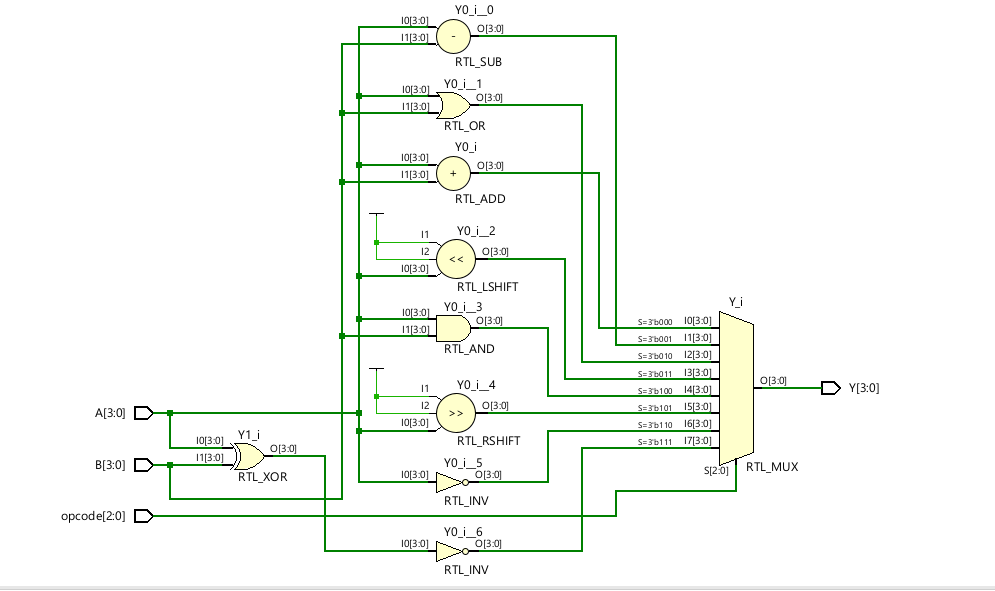
\includegraphics[width=0.9\textwidth]{images/15_rtl.png}
    \caption{RTL Schematic -- Design of a 4-bit Arithmetic Logic Unit}
    \label{fig:15_rtl}
\end{figure}

%----------------------------------------
\section{Verilog Design Code}

\begin{verilogbox}
\begin{lstlisting}
module alu(
    input wire [3:0] A,
    input wire [3:0] B,
    input wire [2:0] opcode,
    output reg [3:0] Y
);

    always @(*) begin
        case(opcode)
            3'b000: Y = A + B;
            3'b001: Y = A - B;
            3'b010: Y = A & B;
            3'b011: Y = A | B;
            3'b100: Y = ~A;
            3'b101: Y = A << 1;
            3'b110: Y = A >> 1;
            default: Y = 4'b0000;
        endcase
    end

endmodule
\end{lstlisting}
\end{verilogbox}

%----------------------------------------
\section{Testbench Code}

\begin{verilogbox}
\begin{lstlisting}
module alu_tb;

    reg [3:0] A;
    reg [3:0] B;
    reg [2:0] opcode;

    wire [3:0] Y;

    alu uut (
        .A(A),
        .B(B),
        .opcode(opcode),
        .Y(Y)
    );

    integer i;

    initial begin

        $monitor("Time = %0t | Opcode = %b | A = %b | B = %b | Y = %b",
                 $time, opcode, A, B, Y);

        A = 4'b0101;
        B = 4'b0011;

        for (i = 0; i < 8; i = i + 1) begin
            opcode = i[2:0];
            #10;
        end

        $finish;

    end

endmodule
\end{lstlisting}
\end{verilogbox}

%----------------------------------------
\section{Simulation Results}

\begin{figure}[H]
    \centering
    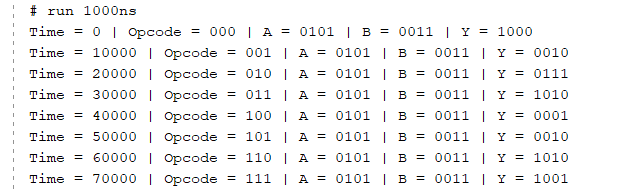
\includegraphics[width=1.2\textwidth]{images/15_sim.png}
    \caption{Simulation Waveform -- Design of a 4-bit Arithmetic Logic Unit}
    \label{fig:15_wave}
\end{figure}

\vspace{0.5cm}

\section{Results and Observations}

The 4-bit Arithmetic Logic Unit was successfully implemented using behavioral modeling in Verilog HDL.

The ALU successfully performed arithmetic, logical, and shift operations according to the applied opcode. For the selected opcode values, the output changed according to the corresponding operation specified in the functional table.

It was observed that the addition and subtraction operations performed arithmetic operations on the two 4-bit inputs, while the AND and OR operations performed bitwise logical operations. The NOT operation complemented all four bits of input $A$.

The left-shift operation shifted the bits of $A$ by one position towards the most significant bit, while the right-shift operation shifted the bits towards the least significant bit.

The simulation results were consistent with the expected outputs for the respective opcode values.


\section{Conclusion}

A 4-bit Arithmetic Logic Unit was successfully designed and implemented using behavioral modeling in Verilog HDL. The designed ALU was capable of performing arithmetic, logical, and shift operations based on a 3-bit opcode.

The simulation verified the correct operation of addition, subtraction, AND, OR, NOT, left-shift, and right-shift functions. The experiment demonstrated how multiple operations can be combined into a single combinational circuit and selected using control signals.

\section{Sources of Error}

\begin{itemize}
    \item Incorrect opcode assignment may cause an unintended operation to be selected.
    \item Incorrect implementation of the arithmetic or logical operation may result in an incorrect output.
    \item Since the output is only 4 bits wide, overflow during addition may be discarded.

\end{itemize}


%-------------------------------------------
\chapter{Realization of D Latch and Master-Slave D Flip-Flop Using NAND Gates}
\label{ch:exp7}

\section{Objective}

To design and verify a gated \textbf{D Latch} and a negative/positive edge-triggered \textbf{Master-Slave D Flip-Flop} using structural NAND gate modeling in Verilog HDL, and validate their operation via simulation.

\section{Theory}

A \textbf{D Latch} is a level-sensitive storage element. When the enable signal ($EN$) is HIGH, the output $Q$ follows the data input $D$ (transparent mode). When $EN$ is LOW, the latch retains its previous state (storage mode). A basic gated D latch constructed using four NAND gates avoids the invalid state of an SR latch by feeding $D$ and its complement $\overline{D}$ into the set and reset paths.

A \textbf{Master-Slave D Flip-Flop} is an edge-triggered storage element formed by cascading two gated D latches in series:
\begin{enumerate}
    \item \textbf{Master Latch:} Enabled on one level of the clock (e.g., $CLK = 1$).
    \item \textbf{Slave Latch:} Enabled on the opposite level of the clock (e.g., $\overline{CLK} = 0 \rightarrow 1$ via an inverter).
\end{enumerate}

Because the two stages are enabled on complementary clock phases, data is isolated from input to output simultaneously, eliminating transparency and providing clean edge-triggered sampling.

\section{Truth Table}

\begin{table}[H]
    \centering
    \caption{Function Table -- Gated D Latch and Edge-Triggered D Flip-Flop}
    \begin{tabular}{|c|c|c|c|l|}
        \hline
        \textbf{Circuit} & \textbf{Clock / Enable} & \textbf{Data ($D$)} & \textbf{Output ($Q_{next}$)} & \textbf{Operation} \\
        \hline
        \multirow{3}{*}{D Latch} & 0 & X & $Q$ & Hold (No Change) \\
        \cline{2-5}
        & 1 & 0 & 0 & Reset \\
        \cline{2-5}
        & 1 & 1 & 1 & Set (Transparent) \\
        \hline
        \multirow{3}{*}{D Flip-Flop} & 0, 1, Falling Edge & X & $Q$ & Memory / Inactive \\
        \cline{2-5}
        & $\uparrow$ (Rising Edge) & 0 & 0 & Reset \\
        \cline{2-5}
        & $\uparrow$ (Rising Edge) & 1 & 1 & Set \\
        \hline
    \end{tabular}
\end{table}

\vspace{0.5cm}

\section{Software Tools}

Icarus Verilog, Yosys (Design Entry, RTL Analysis and Simulation), GTKWave (Waveform Viewer)

\section{Procedure}

\begin{enumerate}
    \item Create a new RTL project in Vivado.
    \item Implement a sub-module for a basic 2-input NAND gate or use Verilog gate primitives (\texttt{nand}).
    \item Construct the gated D Latch module using structural gate-level interconnects.
    \item Instantiate two instances of the D Latch (Master and Slave) with an inverter on the clock path to create the edge-triggered D Flip-Flop.
    \item Generate and inspect the synthesized RTL schematic.
    \item Write a testbench to toggle $D$ while $EN$/$CLK$ changes levels to verify level-sensitivity versus edge-triggering.
    \item Run behavioral simulation and verify that latch transparency occurs only during enable HIGH, while the flip-flop updates strictly on clock edges.
\end{enumerate}

%----------------------------------------
\section{RTL Diagram}
\begin{figure}
    \centering
    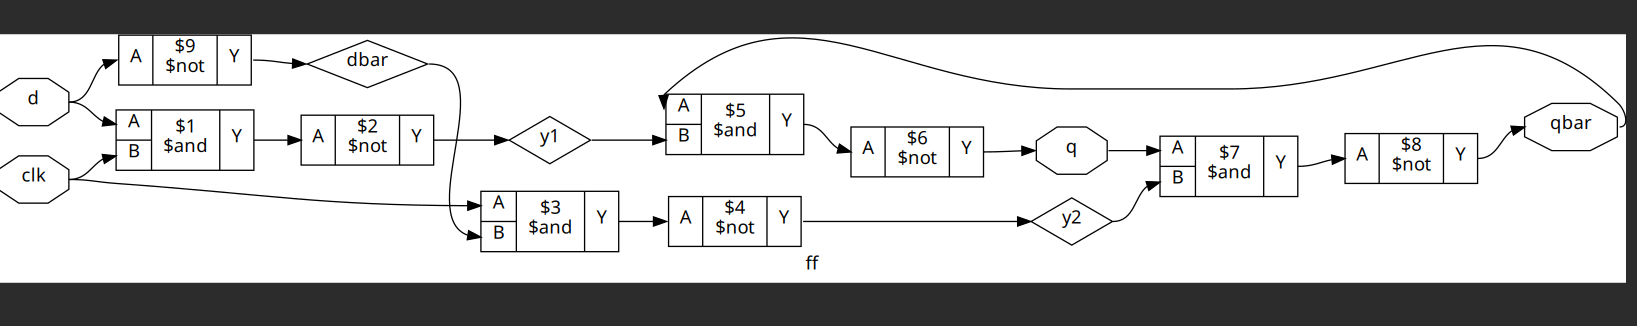
\includegraphics[width=1\linewidth]{images/16_latch_yosys.png}
   \caption{RTL Schematic of Master-Slave D Flip-Flop}
    \label{fig:placeholder}
\end{figure}

%----------------------------------------
\section{Verilog Design Code}

\begin{verilogbox}
\begin{lstlisting}
module nand_d_latch (
    input  wire A,
    input  wire B,
    input  wire D,
    input  wire CLK,
    output wire NAND_Y,
    output reg  Q
);

    assign NAND_Y = ~(A & B);

    always @(*) begin
        if (CLK)
            Q = D;
    end

endmodule

\end{lstlisting}
\end{verilogbox}

%----------------------------------------
\section{Testbench Code}

\begin{verilogbox}
\begin{lstlisting}
`timescale 1ns / 1ps

module d_ff_ms_tb;
    reg D;
    reg CLK;
    wire Q, Qbar;

    d_ff_ms uut (
        .D(D),
        .CLK(CLK),
        .Q(Q),
        .Qbar(Qbar)
    );

    // Generate 20ns clock (50 MHz)
    always #10 CLK = ~CLK;

    initial begin
        CLK = 0;
        D = 0;

        $monitor("Time = %0t | CLK = %b | D = %b | Q = %b | Qbar = %b", 
                 $time, CLK, D, Q, Qbar);

        #15 D = 1;
        #10 D = 0;
        #12 D = 1;
        #15 D = 0;
        #20 D = 1;
        #20;
        $finish;
    end
endmodule
\end{lstlisting}
\end{verilogbox}

%----------------------------------------
\section{Simulation Results}
\begin{figure}
    \centering
    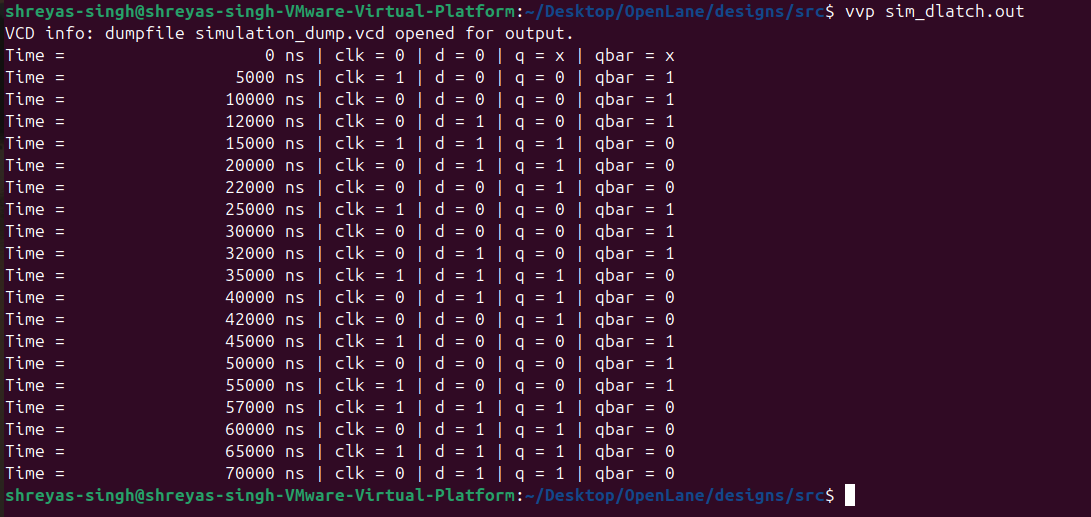
\includegraphics[width=1.0\linewidth]{images/16_latch_vvp.png}
    \caption{Caption}
    \label{fig:placeholder}
\end{figure}

\begin{figure}
    \centering
    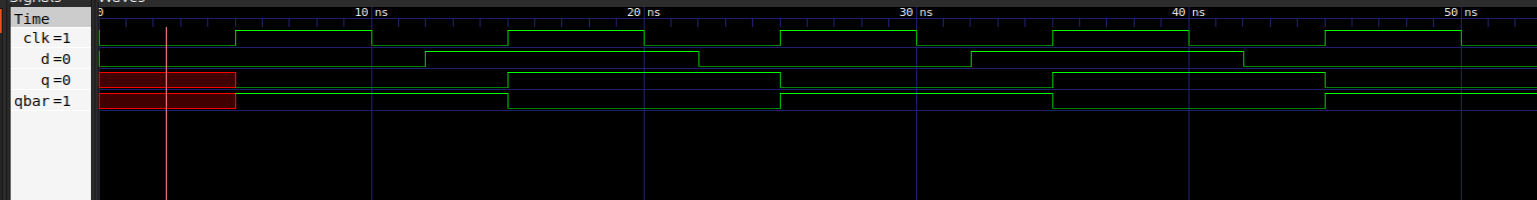
\includegraphics[width=1.2\linewidth]{images/16_latch_gtk.png}
    \caption{Simulation Waveform -- Master-Slave D Flip-Flop}
    \label{fig:placeholder}
\end{figure}


\vspace{0.5cm}

\section{Results and Observations}

The D Latch exhibited level sensitivity: while enable was HIGH, the output followed changes on the data input immediately. In contrast, the Master-Slave D Flip-Flop isolated output transitions to the clock edge, completely suppressing glitching or input variations occurring during steady clock phases.

\vspace{0.5cm}

\section{Conclusion}

A structural gate-level D Latch and Master-Slave D Flip-Flop were constructed using cross-coupled NAND networks. The fundamental operational difference between level-triggered latch transparency and edge-triggered storage was verified through timing simulations.

\section{Sources of Error}

\begin{itemize}
    \item Undefined outputs ($X$) during simulation initialization due to cross-coupled loops without a dedicated reset.
    \item Incorrect port binding between master and slave clock phases.
    \item Race conditions and glitch hazards caused by structural feedback loops in behavioral simulators.
\end{itemize}


%----------------------------------------


%----------------------------------------
\chapter{Analysis of Blocking and Non-Blocking Assignments in Verilog HDL}
\label{ch:exp8}

\section{Objective}

To implement shift register architectures using both \textbf{Blocking (\texttt{=})} and \textbf{Non-Blocking (\texttt{<=})} procedural assignments, and analyze the resulting hardware synthesis and simulation races.

\section{Theory}

Verilog provides two procedural assignment operators inside \texttt{always} blocks:
\begin{enumerate}
    \item \textbf{Blocking Assignment (\texttt{=}):} Evaluated and assigned immediately in sequential order. The execution of the subsequent statement is blocked until the current assignment completes. In sequential circuits, this can collapse cascaded registers into a single register stage.
    \item \textbf{Non-Blocking Assignment (\texttt{<=}):} Evaluates the right-hand side (RHS) expressions of all statements concurrently at the beginning of the time step, and schedules assignments to the left-hand side (LHS) variables at the end of the current evaluation event. This models true concurrent hardware operations like edge-triggered pipeline registers.
\end{enumerate}

\section{Truth Table / Comparative Mapping}

\begin{table}[H]
    \centering
    \caption{Behavioral Comparison across Successive Clock Cycles}
    \begin{tabular}{|c|c|c|c|c|}
        \hline
        \textbf{Architecture} & \textbf{Cycle 0} & \textbf{Cycle 1 ($D=1$)} & \textbf{Cycle 2 ($D=0$)} & \textbf{Synthesized Hardware} \\
        \hline
        Blocking (\texttt{=}) & $Q_1 Q_2 Q_3 = 000$ & $Q_1 Q_2 Q_3 = 111$ & $Q_1 Q_2 Q_3 = 000$ & Single Register (Collapsing) \\
        \hline
        Non-Blocking (\texttt{<=}) & $Q_1 Q_2 Q_3 = 000$ & $Q_1 Q_2 Q_3 = 100$ & $Q_1 Q_2 Q_3 = 010$ & 3-Stage Shift Register \\
        \hline
    \end{tabular}
\end{table}

\vspace{0.5cm}

\section{Software Tools}

Xilinx Vivado 2025.1 (Design Entry, RTL Analysis and Simulation), GTKWave (Waveform Viewer)

\section{Procedure}

\begin{enumerate}
    \item Create two distinct Verilog design files: one modeling a 3-stage shift register with blocking statements and another with non-blocking statements.
    \item Synthesize and run RTL analysis on both files.
    \item Compare the inferred gate schematics: confirm whether registers collapse or pipeline correctly.
    \item Build a common testbench applying a single-cycle pulse on the data input line.
    \item Observe the latency of propagation across stages $Q_1 \rightarrow Q_2 \rightarrow Q_3$.
\end{enumerate}

%----------------------------------------


%----------------------------------------
\section{Verilog Design Code}

\begin{verilogbox}
\begin{lstlisting}
// Module exhibiting blocking assignment side-effects
module shift_blocking(
    input wire clk,
    input wire in,
    output reg q1, q2, q3
);
    always @(posedge clk) begin
        q1 = in;
        q2 = q1;
        q3 = q2;
    end
endmodule

// Module modeling standard concurrent register transfers
module shift_nonblocking(
    input wire clk,
    input wire in,
    output reg q1, q2, q3
);
    always @(posedge clk) begin
        q1 <= in;
        q2 <= q1;
        q3 <= q2;
    end
endmodule
\end{lstlisting}
\end{verilogbox}

%----------------------------------------
\section{Testbench Code}

\begin{verilogbox}
\begin{lstlisting}
`timescale 1ns / 1ps

module assignment_tb;
    reg clk;
    reg in;
    wire q1_b, q2_b, q3_b;
    wire q1_nb, q2_nb, q3_nb;

    shift_blocking uut_b (
        .clk(clk), .in(in),
        .q1(q1_b), .q2(q2_b), .q3(q3_b)
    );

    shift_nonblocking uut_nb (
        .clk(clk), .in(in),
        .q1(q1_nb), .q2(q2_nb), .q3(q3_nb)
    );

    always #5 clk = ~clk;

    initial begin
        clk = 0;
        in = 0;

        #12 in = 1;
        #10 in = 0;
        #30;
        $finish;
    end
endmodule
\end{lstlisting}
\end{verilogbox}

%----------------------------------------
\section{Simulation Results}
\begin{figure}
    \centering
    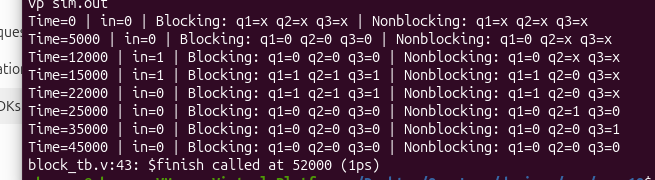
\includegraphics[width=1.2\linewidth]{17_rtl.png}
   \caption{Truth table realization: Shift Delay Comparison}
    \label{fig:placeholder}
\end{figure}

\vspace{0.5cm}

\section{Results and Observations}

In the module using blocking assignments, data shifted through all three registers in a single clock cycle because assignments took effect instantaneously down the execution flow. In contrast, the non-blocking implementation preserved cycle-by-cycle pipelining, shifting the data pulse by exactly one clock cycle per stage.

\vspace{0.5cm}

\section{Conclusion}

Non-blocking assignments (\texttt{<=}) are mandatory for synchronous edge-triggered logic to ensure deterministic multi-register transfers. Blocking assignments (\texttt{=}) should be reserved for combinational logic blocks.

\section{Sources of Error}

\begin{itemize}
    \item Mixing blocking and non-blocking statements within the same sequential \texttt{always} block.
    \item Ordering sensitivity when using blocking assignments in edge-triggered processes.
    \item Simulator event queue scheduling mismatches between different simulator tools.
\end{itemize} 

%----------------------------------------
%----------------------------------------
\chapter{Hamming Weight Calculation}
\label{ch:pdf18}

\section{Objective}

To design and verify a circuit to calculate the \textbf{Hamming weight} (number of logic 1s) of an 8-bit input using Verilog HDL and validate its functionality through simulation.

\section{Theory}

The Hamming weight of a binary word is the number of bits that are set to 1. For an 8-bit input, the Hamming weight can range from 0 to 8.

The circuit examines each bit of the input and calculates the total number of bits having logic value 1. Since the maximum possible count is 8, a 4-bit output is sufficient to represent the result.

For an input
\[
X = X_7X_6X_5X_4X_3X_2X_1X_0,
\]
the Hamming weight is

\[
HW(X) = X_7 + X_6 + X_5 + X_4 + X_3 + X_2 + X_1 + X_0.
\]

The design is implemented as a combinational circuit, so the output changes whenever the input changes.

\section{Truth Table}

For an 8-bit input, a complete truth table would contain $2^8=256$ combinations. Therefore, representative input combinations are shown below.

\begin{table}[H]
    \centering
    \begin{tabular}{|c|c|}
        \hline
        \textbf{8-bit Input} & \textbf{Hamming Weight} \\
        \hline
        00000000 & 0 \\
        \hline
        00000001 & 1 \\
        \hline
        00000011 & 2 \\
        \hline
        00000111 & 3 \\
        \hline
        00001111 & 4 \\
        \hline
        00111111 & 6 \\
        \hline
        01111111 & 7 \\
        \hline
        11111111 & 8 \\
        \hline
    \end{tabular}
    \caption{Representative truth table for Hamming weight calculation}
    \label{tab:hamming_weight}
\end{table}

\section{Software Tools}

\begin{itemize}
    \item \textbf{Verilog HDL} -- RTL design and testbench development.
    \item \textbf{Icarus Verilog} -- RTL simulation.
    \item \textbf{GTKWave} -- Simulation waveform visualization.
    \item \textbf{Yosys} -- RTL synthesis and logic optimization.
    \item \textbf{OpenLane} -- RTL-to-gate-level design flow.
\end{itemize}

\section{Procedure}

\begin{enumerate}
    \item Write the Verilog RTL module for the 8-bit Hamming weight calculator.
    \item Implement the combinational logic required to count the number of logic 1s.
    \item Write a Verilog testbench to apply different 8-bit input patterns.
    \item Compile the RTL design and testbench using Icarus Verilog.
    \item Run the simulation and generate the VCD waveform file.
    \item View the input and output waveforms using GTKWave.
    \item Verify the calculated Hamming weight for the applied test cases.
    \item Use Yosys to synthesize the RTL design and inspect the synthesized representation.
    \item Run the RTL design through the OpenLane flow for synthesis and design verification.
\end{enumerate}

%----------------------------------------
\section{Verilog Design Code}

\begin{verilogbox}
\begin{lstlisting}
`timescale 1ns/1ps

module hamming_weight (
    input  wire [7:0] data_in,
    output reg  [3:0] count
);

    integer i;

    always @(*) begin
        count = 4'b0000;

        for (i = 0; i < 8; i = i + 1) begin
            count = count + data_in[i];
        end
    end

endmodule
\end{lstlisting}
\end{verilogbox}

%----------------------------------------
\section{Testbench Code}

\begin{verilogbox}
\begin{lstlisting}
`timescale 1ns/1ps

module hamming_weight_tb;

    reg  [7:0] data_in;
    wire [3:0] count;

    hamming_weight uut (
        .data_in(data_in),
        .count(count)
    );

    initial begin

        $dumpfile("hamming_weight.vcd");
        $dumpvars(0, hamming_weight_tb);

        $monitor("Time = %0t | Input = %b | Hamming Weight = %0d",
                 $time, data_in, count);

        data_in = 8'b00000000;
        #10;

        data_in = 8'b00000001;
        #10;

        data_in = 8'b00000011;
        #10;

        data_in = 8'b00000111;
        #10;

        data_in = 8'b00001111;
        #10;

        data_in = 8'b00111111;
        #10;

        data_in = 8'b01111111;
        #10;

        data_in = 8'b11111111;
        #10;

        data_in = 8'b10101010;
        #10;

        data_in = 8'b11001100;
        #10;

        $finish;
    end

endmodule
\end{lstlisting}
\end{verilogbox}

%----------------------------------------
\section{Simulation Results}

\begin{figure}
    \centering
    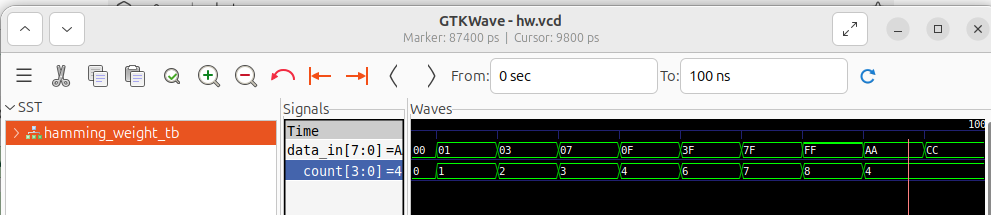
\includegraphics[width=1.1\linewidth]{images/18_gtk.v.png}
    \caption{Output of the gtkwave}
    \label{fig:placeholder}
\end{figure}
\vspace{0.5cm}
\begin{figure}
    \centering
    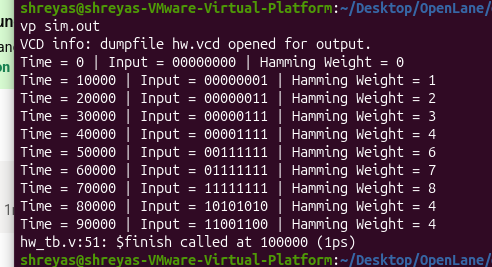
\includegraphics[width=1.1\linewidth]{images/18_sim.png}
    \caption{Truth table realization}
    \label{fig:placeholder}
\end{figure}
\vspace{0.5cm}
\section{Results and Observations}

\begin{itemize}
    \item The circuit successfully calculates the number of logic 1s present in the 8-bit input.
    \item The output ranges from 0 to 8, requiring 4 bits for representation.
    \item For an input of \texttt{11111111}, the output is 8.
    \item For an input of \texttt{00000000}, the output is 0.
    \item The output changes combinationally whenever the input changes.
    \item The functionality was verified through RTL simulation using Icarus Verilog and GTKWave.
\end{itemize}

\section{Conclusion}

An 8-bit Hamming weight calculator was successfully designed using Verilog HDL. The circuit determines the number of bits set to logic 1 and produces the corresponding count as a 4-bit output. The design was verified through simulation and synthesized using the RTL digital design flow.

\section{Sources of Error}

\begin{itemize}
    \item Incorrect bit indexing may result in some input bits not being counted.
    \item Insufficient output width may cause incorrect representation of the maximum count.
    \item Errors in the combinational logic may produce an incorrect Hamming weight.
    \item Incorrect testbench input patterns may lead to incomplete verification.
\end{itemize}


%----------------------------------------
\chapter{Design of a Leading-Zero Detector}
\label{ch:pdf19}

\section{Objective}

To design and verify a \textbf{leading-zero detector} that scans an 8-bit input from the MSB and determines the number of consecutive zeros before the first logic 1 using Verilog HDL and validate its functionality through simulation.

\section{Theory}

A leading-zero detector (LZD) determines the number of consecutive zero bits starting from the most significant bit (MSB) of a binary word. The scanning operation continues toward the least significant bit (LSB) and stops when the first logic 1 is encountered.

For an 8-bit input, the number of leading zeros can range from 0 to 8. A 4-bit output is therefore sufficient to represent the count.

For example:

\begin{itemize}
    \item \texttt{10110010} has 0 leading zeros.
    \item \texttt{00110110} has 2 leading zeros.
    \item \texttt{00001001} has 4 leading zeros.
    \item \texttt{00000001} has 7 leading zeros.
    \item \texttt{00000000} has 8 leading zeros.
\end{itemize}

An additional \texttt{valid} output is used to indicate whether a logic 1 exists in the input. This removes the ambiguity between a valid count and the all-zero input.

\section{Truth Table}

A complete truth table for an 8-bit input contains 256 combinations. Representative cases are shown below.

\begin{table}[H]
    \centering
    \begin{tabular}{|c|c|c|}
        \hline
        \textbf{Input} & \textbf{Leading Zeros} & \textbf{Valid} \\
        \hline
        10000000 & 0 & 1 \\
        \hline
        01000000 & 1 & 1 \\
        \hline
        00100000 & 2 & 1 \\
        \hline
        00010000 & 3 & 1 \\
        \hline
        00001000 & 4 & 1 \\
        \hline
        00000100 & 5 & 1 \\
        \hline
        00000010 & 6 & 1 \\
        \hline
        00000001 & 7 & 1 \\
        \hline
        00000000 & 8 & 0 \\
        \hline
    \end{tabular}
    \caption{Representative truth table for the leading-zero detector}
    \label{tab:lzd}
\end{table}

\section{Software Tools}

\begin{itemize}
    \item \textbf{Verilog HDL} -- RTL design and testbench development.
    \item \textbf{Icarus Verilog} -- RTL simulation.
    \item \textbf{GTKWave} -- Simulation waveform visualization.
    \item \textbf{Yosys} -- RTL synthesis and logic optimization.
    \item \textbf{OpenLane} -- RTL-to-gate-level design flow.
\end{itemize}

\section{Procedure}

\begin{enumerate}
    \item Write the Verilog RTL module for the 8-bit leading-zero detector.
    \item Implement combinational logic to scan the input from MSB to LSB.
    \item Stop counting when the first logic 1 is encountered.
    \item Generate the leading-zero count and validity indication.
    \item Write a Verilog testbench with representative input patterns.
    \item Compile and simulate the design using Icarus Verilog.
    \item Generate the VCD waveform and inspect it using GTKWave.
    \item Verify the leading-zero count for each test case.
    \item Synthesize the RTL using Yosys and inspect the synthesized representation.
    \item Run the RTL design through the OpenLane flow.
\end{enumerate}

%----------------------------------------
\section{RTL Diagram}
\begin{figure}
    \centering
    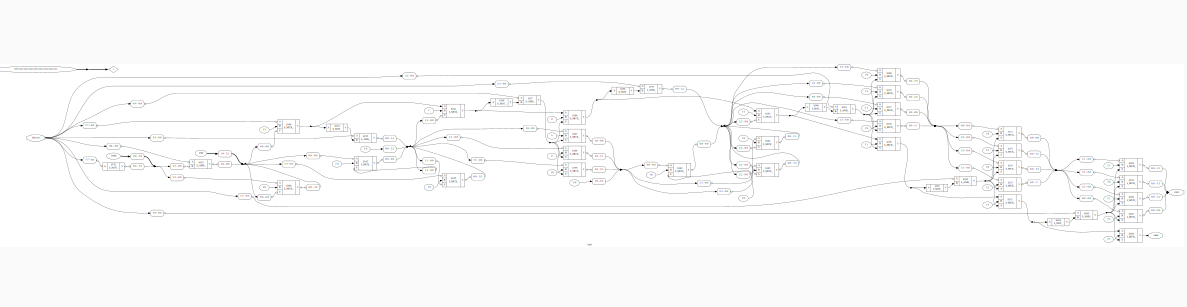
\includegraphics[width=1.0\linewidth]{19_rtl.png}
   \caption{RTL Schematic -- Design of a Leading-Zero Detector}
    \label{fig:placeholder}
\end{figure}

%----------------------------------------
\section{Verilog Design Code}

\begin{verilogbox}
\begin{lstlisting}
`timescale 1ns/1ps

module leading_zero_detector (
    input  wire [7:0] data_in,
    output reg  [3:0] count,
    output reg        valid
);

    integer i;

    always @(*) begin
        count = 4'd8;
        valid = 1'b0;

        for (i = 7; i >= 0; i = i - 1) begin
            if (data_in[i] == 1'b1 && valid == 1'b0) begin
                count = 7 - i;
                valid = 1'b1;
            end
        end
    end

endmodule
\end{lstlisting}
\end{verilogbox}

%----------------------------------------
\section{Testbench Code}

\begin{verilogbox}
\begin{lstlisting}
`timescale 1ns/1ps

module leading_zero_detector_tb;

    reg  [7:0] data_in;
    wire [3:0] count;
    wire       valid;

    leading_zero_detector uut (
        .data_in(data_in),
        .count(count),
        .valid(valid)
    );

    initial begin

        $dumpfile("leading_zero_detector.vcd");
        $dumpvars(0, leading_zero_detector_tb);

        $monitor("Time = %0t | Input = %b | Leading Zeros = %0d | Valid = %b",
                 $time, data_in, count, valid);

        data_in = 8'b10000000;
        #10;

        data_in = 8'b01000000;
        #10;

        data_in = 8'b00100000;
        #10;

        data_in = 8'b00010000;
        #10;

        data_in = 8'b00001000;
        #10;

        data_in = 8'b00000100;
        #10;

        data_in = 8'b00000010;
        #10;

        data_in = 8'b00000001;
        #10;

        data_in = 8'b00000000;
        #10;

        data_in = 8'b00110110;
        #10;

        data_in = 8'b00001101;
        #10;

        $finish;
    end

endmodule
\end{lstlisting}
\end{verilogbox}

%----------------------------------------
\section{Simulation Results}
\begin{figure}
    \centering
    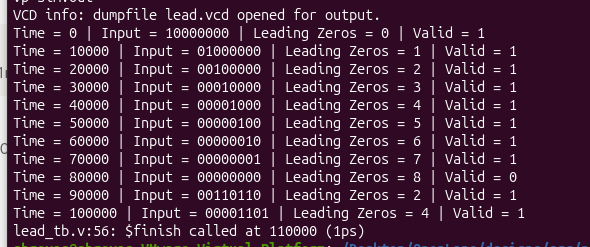
\includegraphics[width=1\linewidth]{19_sim.png}
   \caption{Simulation Waveform -- Design of a Leading-Zero Detector}
    \label{fig:placeholder}
\end{figure}

\vspace{0.5cm}

\section{Results and Observations}

\begin{itemize}
    \item The circuit successfully determines the number of consecutive zeros from the MSB.
    \item The detector stops counting when the first logic 1 is encountered.
    \item An input beginning with logic 1 produces a leading-zero count of 0.
    \item The input \texttt{00000001} produces a leading-zero count of 7.
    \item The all-zero input produces a count of 8 and \texttt{valid}=0.
    \item The functionality was verified using Icarus Verilog and GTKWave.
\end{itemize}

\section{Conclusion}

An 8-bit leading-zero detector was successfully designed using Verilog HDL. The circuit scans the input from the MSB toward the LSB and determines the number of consecutive leading zeros. The design was verified through simulation and synthesized using the RTL digital design flow.

\section{Sources of Error}

\begin{itemize}
    \item Incorrect MSB-to-LSB scanning order can produce an incorrect leading-zero count.
    \item Failure to handle the all-zero input may result in an undefined or incorrect count.
    \item Incorrect output width may prevent representation of the value 8.
    \item Errors in the testbench input patterns may result in incomplete verification.
\end{itemize}


%----------------------------------------
\chapter{Design of a 4-bit Up Counter with Enable and Reset}
\label{ch:pdf20}

\section{Objective}

To design and verify a \textbf{4-bit up counter} with enable and reset inputs using Verilog HDL and validate its functionality through simulation.

\section{Theory}

A counter is a sequential digital circuit that changes its state in response to clock pulses. The 4-bit up counter increments its value by one on every rising edge of the clock when the enable input is HIGH.

When reset is asserted, the counter is set to zero. When enable is LOW, the counter retains its current value.

The counter follows the relation:

\[
Q_{next} =
\begin{cases}
0000, & \text{if reset is HIGH} \\
Q + 1, & \text{if enable is HIGH} \\
Q, & \text{if enable is LOW}
\end{cases}
\]

Since the counter has 4 bits, it counts from 0 to 15. After reaching 15, the next increment causes the counter to wrap around to 0.

\section{Truth Table}

\begin{table}[H]
    \centering
    \begin{tabular}{|c|c|c|}
        \hline
        \textbf{Reset} & \textbf{Enable} & \textbf{Next Counter Value} \\
        \hline
        1 & X & 0000 \\
        \hline
        0 & 0 & Current Value \\
        \hline
        0 & 1 & Current Value + 1 \\
        \hline
    \end{tabular}
    \caption{Function table for the 4-bit up counter}
    \label{tab:up_counter}
\end{table}

\section{Software Tools}

\begin{itemize}
    \item \textbf{Verilog HDL} -- RTL design and testbench development.
    \item \textbf{Icarus Verilog} -- RTL simulation.
    \item \textbf{GTKWave} -- Simulation waveform visualization.
    \item \textbf{Yosys} -- RTL synthesis and logic optimization.
    \item \textbf{OpenLane} -- RTL-to-gate-level design flow.
\end{itemize}

\section{Procedure}

\begin{enumerate}
    \item Write the Verilog RTL module for the 4-bit up counter.
    \item Implement the counter using a positive-edge-triggered clock.
    \item Implement reset functionality to clear the counter to zero.
    \item Implement enable functionality to control whether the counter increments.
    \item Write a Verilog testbench to generate the clock and apply reset and enable conditions.
    \item Compile and simulate the design using Icarus Verilog.
    \item Generate the VCD waveform and view it using GTKWave.
    \item Verify the counter operation for reset, enabled, and disabled conditions.
    \item Synthesize the RTL design using Yosys.
    \item Run the RTL design through the OpenLane flow for synthesis and design verification.
\end{enumerate}

%----------------------------------------
\section{RTL Diagram}
\begin{figure}
    \centering
    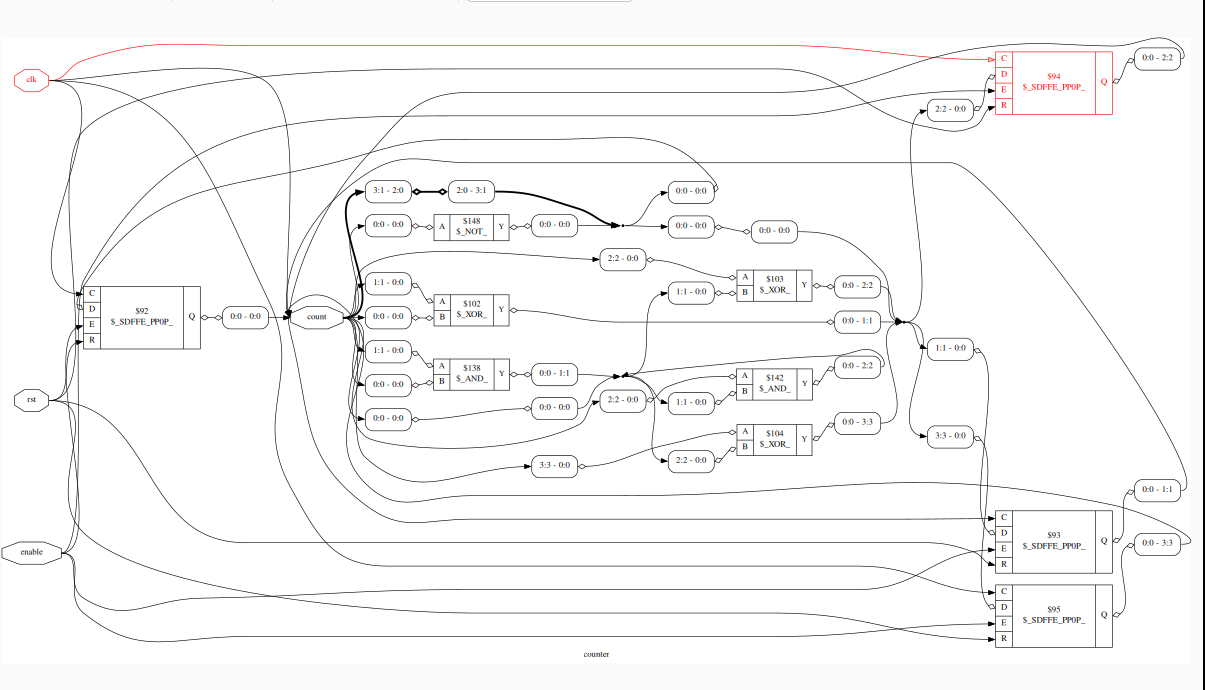
\includegraphics[width=1.1\linewidth]{counter_rtl.png}
    \caption{RTL Schematic -- Design of a 4-bit Up Counter with Enable and Reset}
    \label{fig:placeholder}
\end{figure}

%----------------------------------------
\section{Verilog Design Code}

\begin{verilogbox}
\begin{lstlisting}
`timescale 1ns/1ps

module up_counter (
    input  wire       clk,
    input  wire       rst,
    input  wire       enable,
    output reg  [3:0] count
);

    always @(posedge clk) begin
        if (rst)
            count <= 4'b0000;
        else if (enable)
            count <= count + 4'b0001;
        else
            count <= count;
    end

endmodule
\end{lstlisting}
\end{verilogbox}

%----------------------------------------
\section{Testbench Code}

\begin{verilogbox}
\begin{lstlisting}
`timescale 1ns/1ps

module up_counter_tb;

    reg       clk;
    reg       rst;
    reg       enable;
    wire [3:0] count;

    up_counter uut (
        .clk(clk),
        .rst(rst),
        .enable(enable),
        .count(count)
    );

    // Clock generation
    always #5 clk = ~clk;

    initial begin

        $dumpfile("up_counter.vcd");
        $dumpvars(0, up_counter_tb);

        $monitor("Time = %0t | Reset = %b | Enable = %b | Count = %b (%0d)",
                 $time, rst, enable, count, count);

        clk    = 1'b0;
        rst    = 1'b1;
        enable = 1'b0;

        // Reset counter
        #10;
        rst = 1'b0;

        // Enable counting
        enable = 1'b1;
        #50;

        // Disable counting
        enable = 1'b0;
        #30;

        // Enable counting again
        enable = 1'b1;
        #50;

        // Reset while counter is active
        rst = 1'b1;
        #10;

        rst = 1'b0;
        enable = 1'b1;
        #30;

        $finish;
    end

endmodule
\end{lstlisting}
\end{verilogbox}

%----------------------------------------
\section{Simulation Results}
\begin{figure}
    \centering
    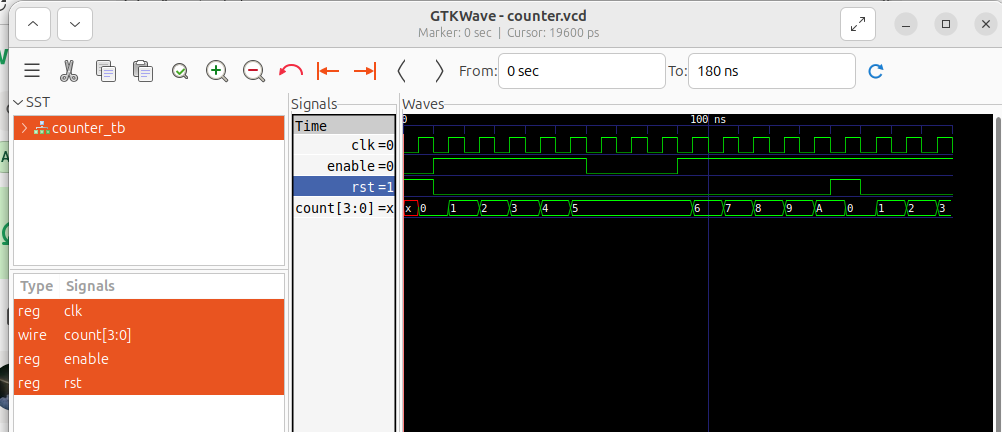
\includegraphics[width=1.2\linewidth]{counter_gtk.png}
    \caption{Simulation Waveform -- Design of a 4-bit Up Counter with Enable and Reset}
    \label{fig:placeholder}
\end{figure}

\vspace{0.5cm}

\section{Results and Observations}

\begin{itemize}
    \item The counter is reset to zero when the reset input is HIGH at a rising clock edge.
    \item When enable is HIGH, the counter increments by one at every rising edge of the clock.
    \item When enable is LOW, the counter retains its previous value.
    \item The 4-bit counter counts from 0 to 15 and wraps around to 0 after reaching 15.
    \item The counter operation was verified through RTL simulation using Icarus Verilog and GTKWave.
    \item The RTL design was synthesized using Yosys and processed through the OpenLane RTL design flow.
\end{itemize}

\section{Conclusion}

A 4-bit synchronous up counter with enable and reset functionality was successfully designed using Verilog HDL. The counter increments on every rising clock edge when enabled, retains its value when disabled, and resets to zero when reset is asserted. The functionality was verified through simulation and the RTL was synthesized using the digital design flow.

\section{Sources of Error}

\begin{itemize}
    \item Incorrect clock or reset behavior can result in an incorrect counter value.
    \item Incorrect enable logic may cause the counter to increment when it should retain its value.
    \item Incorrect counter width may result in unintended behavior during overflow.
    \item Improper testbench timing may cause incorrect interpretation of the counter waveform.
    \item Incomplete reset initialization can lead to an unknown counter state during simulation.
\end{itemize}

%----------------------------------------
\chapter{Sequence Detector for 101 with Overlapping Detection}
\label{ch:pdf21}

\section{Objective}

Design and implementation of a sequence detector that detects the sequence 101 in
a serial input stream. The output goes high as soon as the sequence 101 is detected.
Overlapping detection is allowed, so a new sequence can begin before the previous
sequence has completely finished.

\section{Theory}

The output goes HIGH as soon as 101 is detected. Overlapping is allowed, so a new sequence may begin before the previous one has completely finished.
\begin{figure}
    \centering
    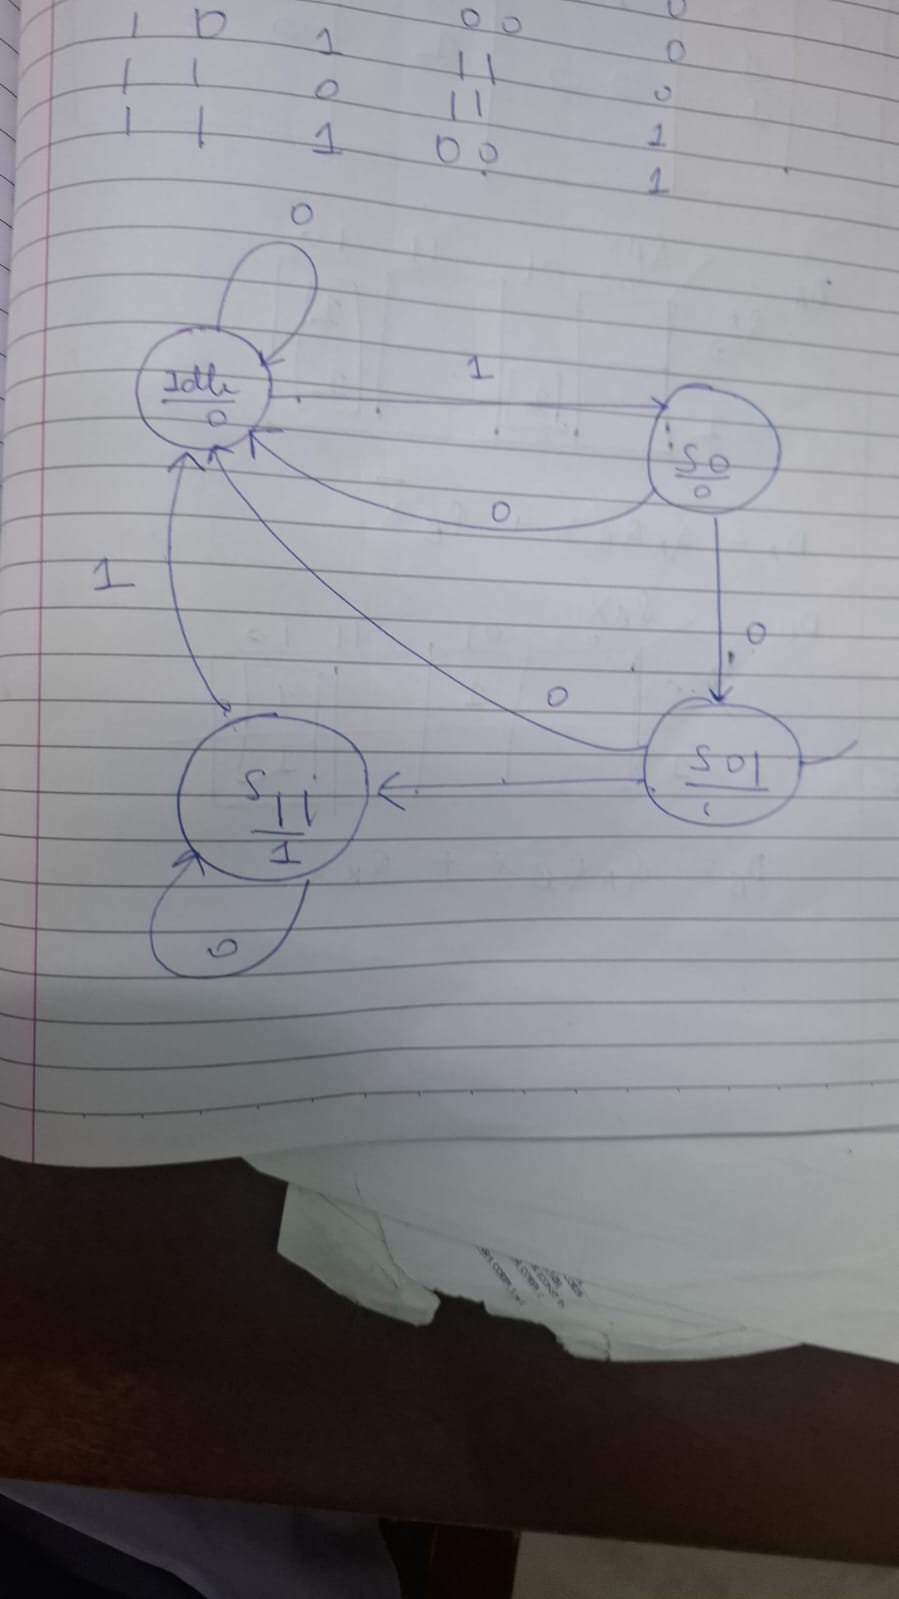
\includegraphics[width=1\linewidth]{22_state.jpg}
    \caption{State Diagram of Moore Machine}
    \label{fig:placeholder}
\end{figure}
\section{Truth Table}

\begin{table}[h]
\centering
\caption{Characteristic Table}
\begin{tabular}{cc|c|cc|c}
\hline
\multicolumn{2}{c|}{Present State} & Input & \multicolumn{2}{c|}{Next State} & Output \\
$Q_1$ & $Q_0$ & $X$ & $Q_1^{+}$ & $Q_0^{+}$ & $Y$ \\
\hline
0 & 0 & 0 & 0 & 0 & 0 \\
0 & 0 & 1 & 0 & 1 & 0 \\
0 & 1 & 0 & 1 & 0 & 0 \\
0 & 1 & 1 & 0 & 0 & 0 \\
1 & 0 & 0 & 0 & 0 & 0 \\
1 & 0 & 1 & 1 & 1 & 0 \\
1 & 1 & 0 & 1 & 1 & 1 \\
1 & 1 & 1 & 0 & 0 & 1 \\
\hline
\end{tabular}
\end{table}
\vspace{3cm}

\section{Software Tools}

Icarus Verilog , GTKWave (Waveform Viewer) , Yosys 

\section{Procedure}

\begin{enumerate}
    \item Create a new RTL project in Vivado.
    \item Write the Verilog module for the design.
    \item Run RTL Analysis and generate the RTL schematic.
    \item Write a testbench to apply the required input combinations.
    \item Run the behavioral simulation and view the waveform in GTKWave.
    \item Verify the outputs against the expected results.
\end{enumerate}

%----------------------------------------
\section{RTL Diagram}
\begin{figure}
    \centering
    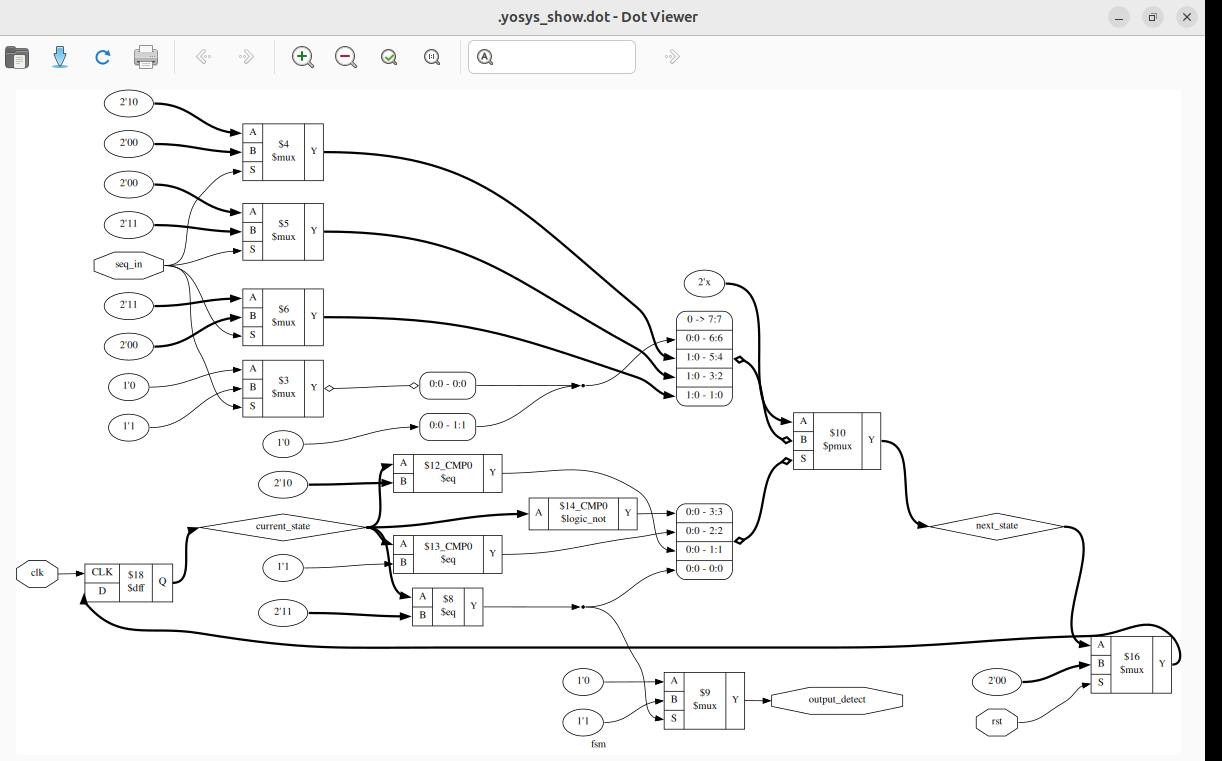
\includegraphics[width=1\linewidth]{21_yosys.png}
    \caption{RTL Schematic -- Sequence Detector for 101 with Overlapping Detection}
    \label{fig:placeholder}
\end{figure}

%----------------------------------------
\section{Verilog Design Code}

\begin{verilogbox}
\begin{lstlisting}
`timescale 1ns/1ps

module fsm(
    input  wire clk,
    input  wire rst,
    input  wire seq_in,
    output reg  output_detect
);

    
    parameter idle  = 2'b00;
    parameter S01  = 2'b01;
    parameter S10 = 2'b10;
    parameter S11 = 2'b11;
    reg [1:0] current_state, next_state;

    //state memory 
    always @(posedge clk) begin
        if (rst)
            current_state <= idle;
        else
            current_state <= next_state;
    end

    // 2. Next-state logic
    always @(*) begin
        case (current_state)
        
            idle:
                next_state = seq_in ? S01 : idle;

            S01:
                next_state = seq_in ? idle : S10 ; 
               
                
            S10:
                next_state = seq_in ? S11 : idle ; 

            S11:
                next_state = seq_in ? idle : S11 ;

            default:
                next_state = idle;

        endcase
    end

    // 3. Output logic
    always @(*) begin
        output_detect = current_state == S11 ? 1'b1 : 1'b0;
    end

endmodule
\end{lstlisting}
\end{verilogbox}

%----------------------------------------
\section{Testbench Code}

\begin{verilogbox}
\begin{lstlisting}
`timescale 1ns/1ps

module fsm_tb();

    reg clk, rst, seq_in;
    wire out_detect;

    fsm uut (
        .clk(clk),
        .rst(rst),
       .seq_in(seq_in),
        .output_detect(out_detect)
    );

    always #5 clk = ~clk;

    initial begin
        $dumpfile("fsm.vcd");
        $dumpvars(1, fsm_tb);

        $monitor("Time = %t | CLK = %b | RST = %b | seq_in = %b | OUT = %b",
                 $time, clk, rst, seq_in, out_detect);

        clk = 0;
        seq_in = 0;

        // Active-high reset
        rst = 1;

        // Allow reset to happen at a rising edge
        #10;

        // Release reset
        rst = 0;

        @(negedge clk) seq_in  = 1 ;
       @(negedge clk) seq_in  = 0;

       @(negedge clk) seq_in  = 0 ;
       @(negedge clk) seq_in  = 1 ;
       @(negedge clk) seq_in  = 0 ;
       @(negedge clk) seq_in  = 1 ;
       @(negedge clk) seq_in  = 1 ;
       @(negedge clk) seq_in  = 0 ;
       
        @(negedge clk) seq_in  = 0 ;
       
      

        $finish;
    end

endmodule
\end{lstlisting}
\end{verilogbox}

%----------------------------------------
\section{Simulation Results}

\begin{figure}
    \centering
    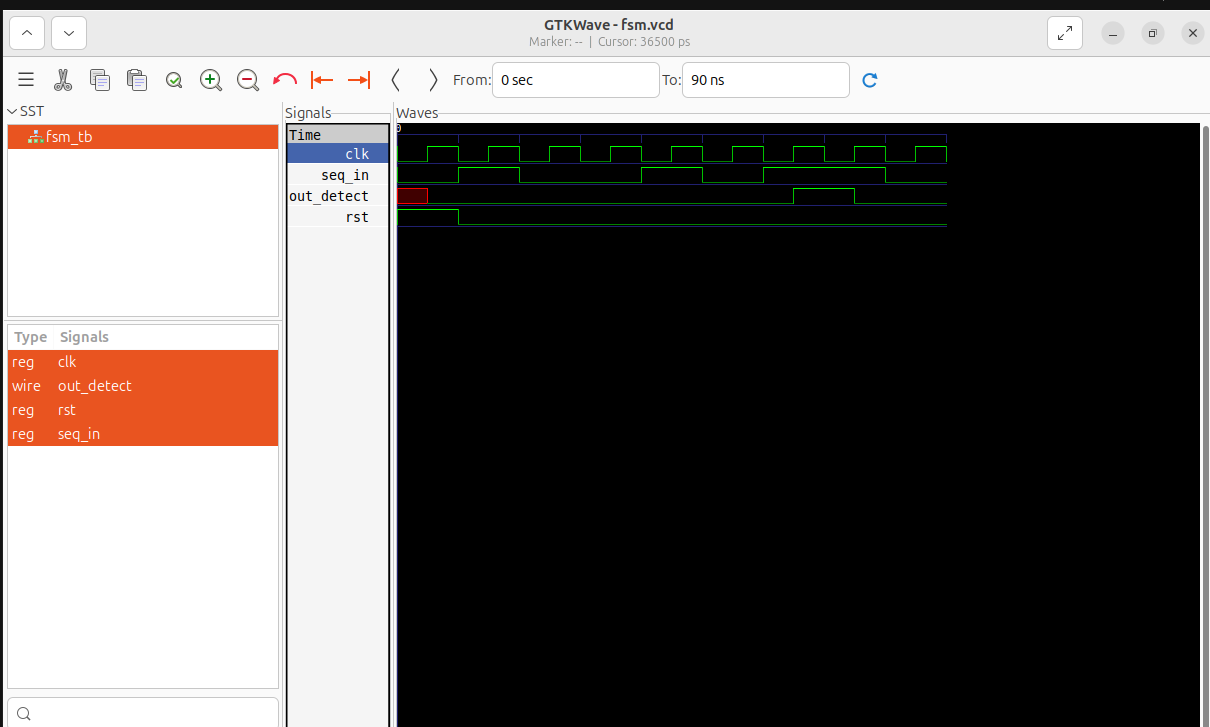
\includegraphics[width=1\linewidth]{21_gtkwave.png}
    \caption{Simulation Waveform -- Sequence Detector for 101 with Overlapping Detection}
    \label{fig:placeholder}
\end{figure}

\begin{figure}
    \centering
    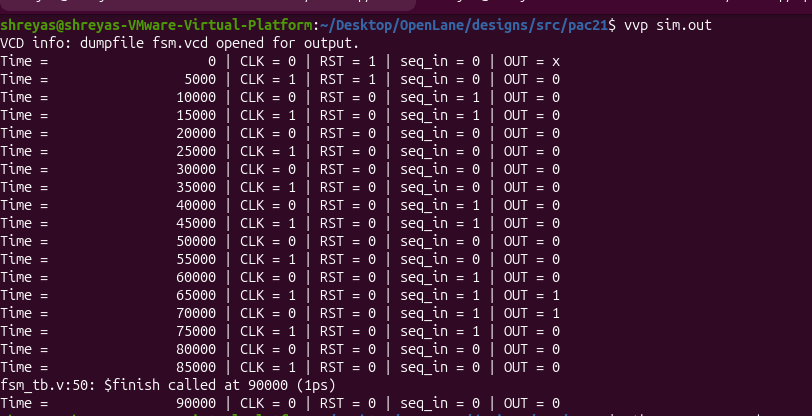
\includegraphics[width=1.0\linewidth]{21_vvp.png}
    \caption{Caption}
    \label{fig:placeholder}
\end{figure}

\section{Results and Observations}

The sequence detector for detecting the serial sequence (101) was successfully designed and implemented using a finite state machine. The circuit correctly monitors the incoming serial bit stream and produces a high output whenever the sequence (101) is detected. Overlapping sequence detection was also implemented, allowing a new sequence to begin before the previous sequence has completely finished.

\section{Conclusion}

A sequence detector for the sequence (101) was successfully designed and simulated using a finite state machine. The detector generates a high output immediately after receiving the complete (101) sequence. 


\section{Sources of Error}

\begin{itemize}
\item Incorrect timing of the serial input bits may result in unexpected state transitions.
\item Improper initialization or reset of the FSM may lead to an incorrect initial state.
\item Errors in the state transition or output logic can cause incorrect sequence detection.
\item Incorrect handling of overlapping sequences may result in missed detections.
\item Simulation timing and testbench errors may affect the observed output waveform.
\end{itemize}

\vspace{2.5cm}


%----------------------------------------
\chapter{Implementation of a Vending Machine Controller}
\label{ch:pdf22}

\section{Objective}

To design and verify a \textbf{vending machine controller} accepting denominations of Rs.\ 5, and  Rs.\ 10 using Verilog HDL and validate its functionality through simulation.



\section{Theory}

The controller tracks the accumulated amount. When it reaches Rs.\ 15 the output is activated. Any denomination received after reaching Rs.\ 15 returns the controller to the initial state.

\section{Truth Table}

\begin{table}[H]
\centering
\caption{State Transition Table for Vending Machine Controller}
\label{tab:vending_fsm}
\begin{tabular}{|c|c|c|c|c|}
\hline
\textbf{Present State} & \textbf{State Code} & 
\textbf{Input = ₹5} & \textbf{Input = ₹10} & \textbf{Output} \\ 
\hline

$S_0$ Idle  & 00 & $S_5$  & $S_{10}$ & 0 \\ 
\hline

$S_5$ (₹5)  & 01 & $S_{10}$ & $S_{15}$ & 0 \\ 
\hline

$S_{10}$ (₹10) & 10 & $S_{15}$ & $S_{15}$ & 0 \\ 
\hline

$S_{15}$ (₹15) & 11 & $S_0$ & $S_0$ & 1 \\ 
\hline

\end{tabular}
\end{table}
\vspace{3cm}

\begin{figure}[H]
\centering

\begin{tikzpicture}[
    ->,
    >=stealth,
    shorten >=1pt,
    auto,
    node distance=3cm,
    semithick
]

\tikzstyle{every state}=[
    draw=black,
    minimum size=1.4cm
]

\node[state, initial] (S0) {$S_0$\newline\scriptsize Idle/Output = 0};
\node[state] (S5) [right of=S0] {\shortstack{$S_5$ \\ \scriptsize Output = 0}};
\node[state] (S10) [right of=S5] {$S_{10}$\\\scriptsize Output = 0};
\node[state] (S15) [right of=S10] {$S_{15}$\\\scriptsize Output = 1};

\path
(S0) edge [above] node {₹5} (S5)
(S0) edge [bend left=20, above] node {₹10} (S10)

(S5) edge [above] node {₹5} (S10)
(S5) edge [bend left=20, above] node {₹10} (S15)

(S10) edge [above] node {₹5} (S15)
(S10) edge [bend left=25, below] node {₹10} (S15)

(S15) edge [bend left=45, below] node {₹5, ₹10} (S0);

\end{tikzpicture}

\caption{Moore State Diagram for Vending Machine Controller}
\label{fig:moore_vending}
\end{figure}

\section{Software Tools}

Icarus Verilog (Design Entry, RTL Analysis and Simulation), GTKWave (Waveform Viewer) Yosys 

\section{Procedure}

\begin{enumerate}
    \item Create a new RTL project .
    \item Write the Verilog module for the design.
    \item Run RTL Analysis and generate the RTL schematic.
    \item Write a testbench to apply the required input combinations.
    \item Run the behavioral simulation and view the waveform in GTKWave.
    \item Verify the outputs against the expected results.
\end{enumerate}

%----------------------------------------
\section{RTL Diagram}

\begin{figure}[H]
    \centering
    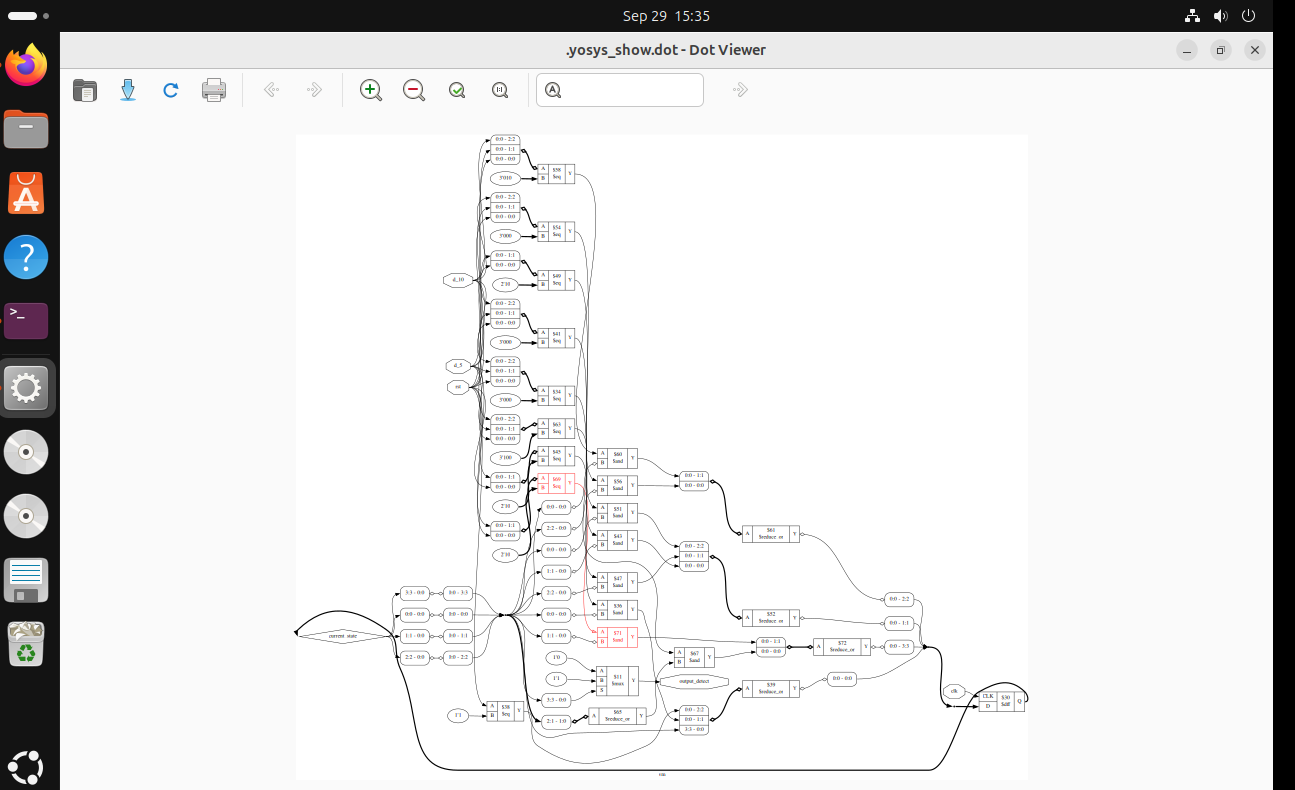
\includegraphics[width=1\linewidth]{images/22_vending_fsm.png}
    \caption{RTL Schematic -- Implementation of a Vending Machine Controller}
\end{figure}

%----------------------------------------
\section{Verilog Design Code}

\begin{verilogbox}
\begin{lstlisting}
`timescale 1ns/1ps

module vm(
    input  wire clk,
    input  wire rst,
    input  wire d_5,d_10,
    output reg  output_detect
);

    
    parameter idle  = 2'b00;
    parameter Rs5  = 2'b01;
    parameter Rs10 = 2'b10;
    parameter Rs15 = 2'b11;
    reg [1:0] current_state, next_state;

    //state memory 
    always @(posedge clk) begin
        if (rst)
            current_state <= idle;
        else
            current_state <= next_state;
    end

    // 2. Next-state logic
    always @(*) begin
        case (current_state)
//Here priority is given to 10 rupee coin, so ternary operator is considered , but in the mid sem such a question be give 
            idle:
                next_state = d_10 ? Rs10 : d_5 ? Rs5 : idle;

            Rs5:
                next_state = d_5 ? Rs10 : d_10 ? Rs15 : Rs5 ;
                
                // next = ( d_5 || d_10 ) ? RS15: rs10;
                
            Rs10:
                next_state = d_5 ? Rs15 : d_10 ? Rs15 : Rs10;

            Rs15:
                next_state = idle;

            default:
                next_state = idle;

        endcase
    end

    // 3. Output logic
    always @(*) begin
        output_detect = current_state == Rs15 ? 1'b1 : 1'b0;
    end

endmodule
\end{lstlisting}
\end{verilogbox}

%----------------------------------------
\section{Testbench Code}

\begin{verilogbox}
\begin{lstlisting}
`timescale 1ns/1ps

module vm_tb;

    reg clk, rst, d_5, d_10;
    wire out_detect;

    vm uut (
        .clk(clk),
        .rst(rst),
        .d_5(d_5),
        .d_10(d_10),
        .output_detect(out_detect)
    );

    always #5 clk = ~clk;

    initial begin
        $dumpfile("vm.vcd");
        $dumpvars(1, vm_tb);

        $monitor("Time = %t | CLK = %b | RST = %b | D5 = %b | D10 = %b | OUT = %b",
                 $time, clk, rst, d_5, d_10, out_detect);

        clk = 0;
        d_5 = 0;
        d_10 = 0;

        // Active-high reset
        rst = 1;

        // Allow reset to happen at a rising edge
        #10;

        // Release reset
        rst = 0;

        // -----------------------------
        // Test 1: 5 + 5 + 5 = 15
        // -----------------------------
        @(negedge clk) d_5 = 1;
        @(negedge clk) d_5 = 0;

        @(negedge clk) d_5 = 1;
        @(negedge clk) d_5 = 0;

        @(negedge clk) d_5 = 1;
        @(negedge clk) d_5 = 0;

        #20;

        // -----------------------------
        // Test 2: denomination after 15
        // should return to idle
        // -----------------------------
        @(negedge clk) d_10 = 1;
        @(negedge clk) d_10 = 0;

        #20;

        // -----------------------------
        // Test 3: 10 + 5 = 15
        // -----------------------------
        @(negedge clk) d_10 = 1;
        @(negedge clk) d_10 = 0;

        @(negedge clk) d_5 = 1;
        @(negedge clk) d_5 = 0;

        #20;

        // -----------------------------
        // Test 4: direct 15
        // -----------------------------
        // Your interface doesn't currently have d_15,
        // so this cannot be tested yet.

        $finish;
    end

endmodule
\end{lstlisting}
\end{verilogbox}

%----------------------------------------
\section{Simulation Results}

\begin{figure}[H]
    \centering
    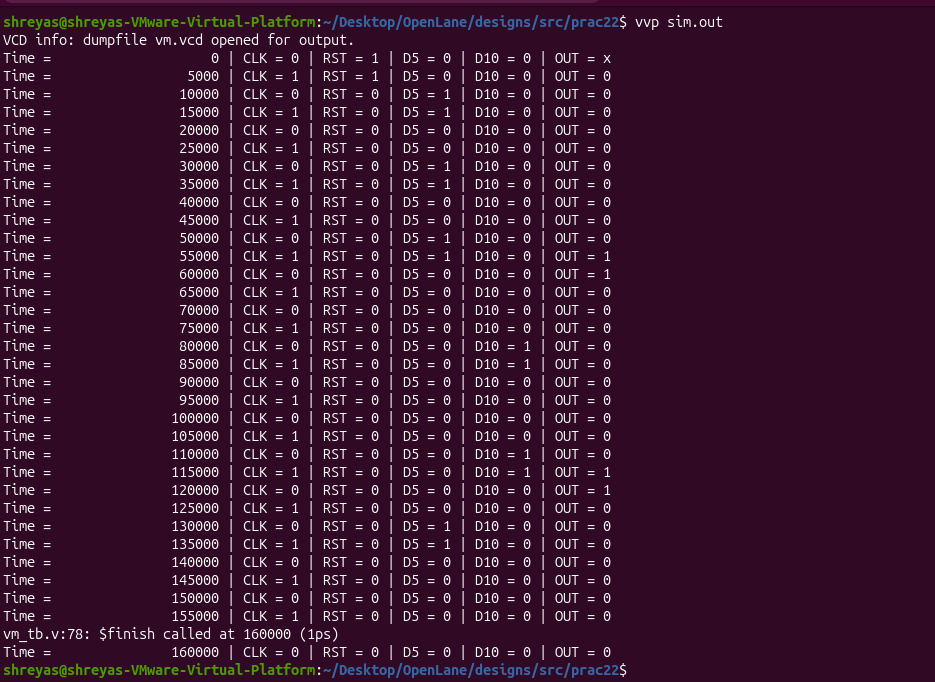
\includegraphics[width=1\linewidth]{images/22_sim.png}
    \caption{Simulation Waveform -- Implementation of a Vending Machine Controller}
\end{figure}

\begin{figure}
    \centering
    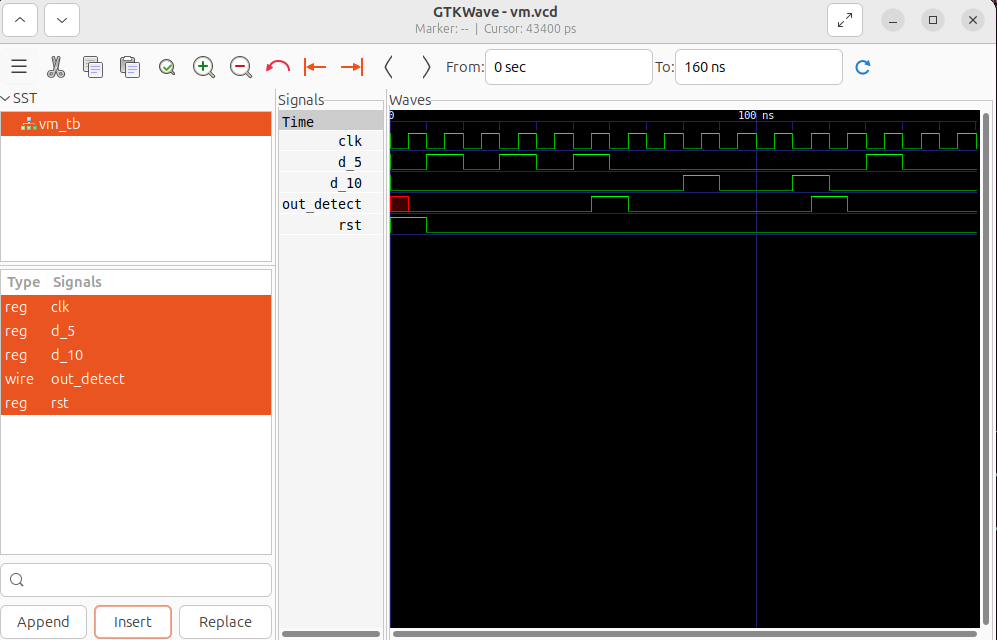
\includegraphics[width=1\linewidth]{images/22_vending.png}
    \caption{Waveform- The output gets flagged upon arrival of 1s}
    \label{fig:placeholder}
\end{figure}

\vspace{0.5cm}

\section{Results and Observations}

The vending machine controller was successfully designed and implemented using a Moore finite state machine. The controller correctly tracks the amount inserted using four states corresponding to ₹0, ₹5, ₹10, and ₹15. The output is activated when the controller reaches the ₹15 state. Any subsequent denomination received after reaching ₹15 causes the controller to return to the initial state.

The state transitions and output behavior were verified through simulation, and the obtained waveform was found to be consistent with the designed state transition table.

\vspace{2cm}

\section{Conclusion}

A Moore finite state machine based vending machine controller was successfully designed and simulated. The controller accepts ₹5 and ₹10 denominations, keeps track of the accumulated amount, and activates the output when the total reaches ₹15. The design was verified using simulation and the expected state transitions and output response were observed.

\vspace{1.5cm}

\section{Sources of Error}

\begin{itemize}
    \item Incorrect input timing during simulation may result in unexpected state transitions.
    \item Improper initialization or reset of the FSM may cause an incorrect initial state.
    \item Errors in state encoding or transition logic can lead to incorrect controller behavior.
    \item Simulation and synthesis tool settings may affect the observed results.
    \item Any mismatch between the testbench input sequence and the intended vending sequence may produce unexpected waveforms.
\end{itemize}

\vspace{2.5cm}

%----------------------------------------
\chapter{Implementation of a Rising-Edge Detector with Digital Switch}
\label{ch:pdf23}

\section{Objective}

To design and implement a \textbf{rising-edge detector} using a digital push button as the input. The design is implemented as a three-block FSM using Verilog HDL, functionally verified through simulation, and synthesized and physically implemented using the OpenLane/OpenROAD digital design flow.

\section{Theory}

A rising-edge detector generates a HIGH output for exactly one clock cycle whenever the input signal changes from $0$ to $1$.

A two-state FSM is used for detecting the transition:

\begin{itemize}
    \item \textbf{LOW state:} Represents that the button was previously LOW.
    \item \textbf{HIGH state:} Represents that the button is currently HIGH.
\end{itemize}

The state transitions are:

\begin{itemize}
    \item LOW $\rightarrow$ LOW when $b=0$
    \item LOW $\rightarrow$ HIGH when $b=1$
    \item HIGH $\rightarrow$ HIGH when $b=1$
    \item HIGH $\rightarrow$ LOW when $b=0$
\end{itemize}

The output is asserted when the FSM is in the LOW state and the current button input is HIGH. Therefore, the output becomes HIGH only during the detection of a $0\rightarrow1$ transition and returns LOW in the following clock cycle even if the button remains pressed.

The design follows the three-block FSM architecture:

\begin{enumerate}
    \item \textbf{State Memory:} Stores the current state using a clocked sequential block.
    \item \textbf{Next-State Logic:} Determines the next FSM state based on the current state and button input.
    \item \textbf{Output Logic:} Generates the rising-edge detection pulse from the current state and input.
\end{enumerate}

\section{State Transition Table}

\begin{table}[H]
    \centering
    \begin{tabular}{|c|c|c|c|}
        \hline
        \textbf{Present State} & \textbf{Button $b$} & \textbf{Next State} & \textbf{Output $out$} \\
        \hline
        LOW  & 0 & LOW  & 0 \\
        \hline
        LOW  & 1 & HIGH & 1 \\
        \hline
        HIGH & 0 & LOW  & 0 \\
        \hline
        HIGH & 1 & HIGH & 0 \\
        \hline
    \end{tabular}
    \caption{State transition table for the rising-edge detector}
    \label{tab:rising_edge_fsm}
\end{table}

\section{Software Tools}

\begin{itemize}
    \item \textbf{Verilog HDL} -- RTL design and testbench development.
    \item \textbf{Yosys} -- RTL synthesis and logic optimization.
    \item \textbf{OpenROAD} -- Physical design and implementation.
    \item \textbf{OpenLane} -- Automated RTL-to-GDSII design flow.
    \item \textbf{Icarus Verilog} -- RTL simulation.
    \item \textbf{GTKWave} -- Simulation waveform visualization.
\end{itemize}

\section{Procedure}

\begin{enumerate}
    \item Create the Verilog RTL module for the rising-edge detector using a three-block FSM architecture.
    
    \item Define the LOW and HIGH states and implement the state-memory block using a positive-edge-triggered clock.
    
    \item Implement the next-state logic using a combinational \texttt{always @(*)} block.
    
    \item Implement the output logic such that the output becomes HIGH only when a rising transition of the button input is detected.
    
    \item Create a Verilog testbench to generate the clock, reset signal, and different button input conditions.
    
    \item Compile and simulate the RTL design using Icarus Verilog.
    
    \item Generate the waveform output and verify the one-clock-cycle detection pulse using GTKWave.
    
    \item Use Yosys to read and synthesize the RTL design and generate the RTL schematic.
    
    \item Configure the design for the OpenLane flow with the required design name, clock definition, and technology parameters.
    
    \item Run the OpenLane/OpenROAD flow to perform synthesis, floorplanning, placement, clock-tree synthesis, routing, and physical implementation.
    
    \item Inspect the generated physical-design results and verify that the design completes the required implementation stages.
\end{enumerate}

%----------------------------------------
\section{RTL Diagram}
\begin{figure}
    \centering
    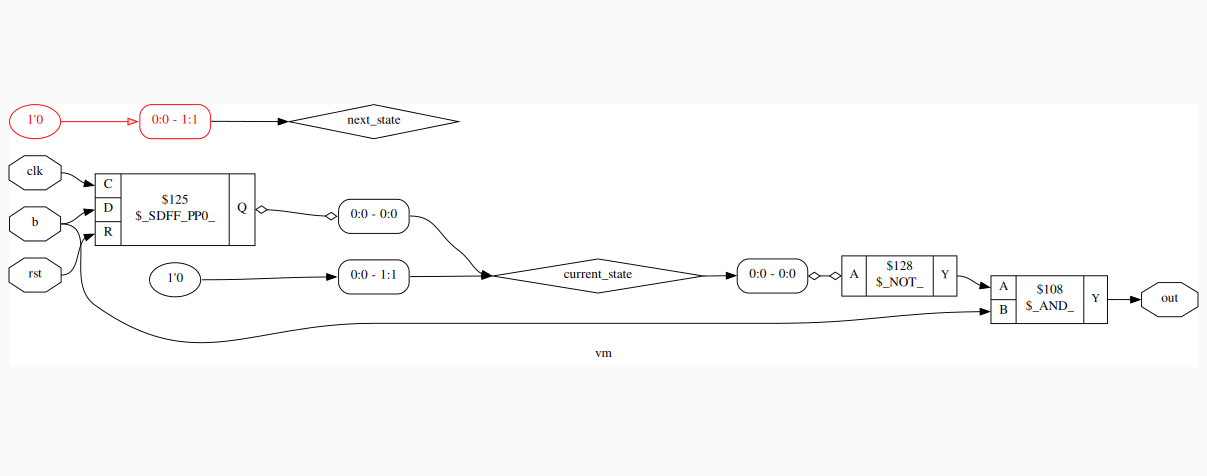
\includegraphics[width=1.0\linewidth]{images/23_rtl.png}
   \caption{RTL Schematic -- Rising-Edge Detector with Digital Switch}
    \label{fig:placeholder}
\end{figure}


%----------------------------------------
\section{Verilog Design Code}

\begin{verilogbox}
\begin{lstlisting}
`timescale 1ns/1ps

module vm(
    input  wire clk,
    input  wire rst,
    input  wire b,
    output reg  out
);

    parameter LOW  = 1'b0;
    parameter HIGH = 1'b1;

    reg current_state, next_state;

    // 1. State memory
    always @(posedge clk) begin
        if (rst)
            current_state <= LOW;
        else
            current_state <= next_state;
    end

    // 2. Next-state logic
    always @(*) begin
        case (current_state)

            LOW:
                next_state = b ? HIGH : LOW;

            HIGH:
                next_state = b ? HIGH : LOW;

            default:
                next_state = LOW;

        endcase
    end

    // 3. Output logic
    always @(*) begin
        if (current_state == LOW && b == 1'b1)
            out = 1'b1;
        else
            out = 1'b0;
    end

endmodule
\end{lstlisting}
\end{verilogbox}

%----------------------------------------
\section{Testbench Code}

\begin{verilogbox}
\begin{lstlisting}
`timescale 1ns/1ps

module vm_tb;

    reg clk;
    reg rst;
    reg b;
    wire out;

    vm uut (
        .clk(clk),
        .rst(rst),
        .b(b),
        .out(out)
    );

    // Clock generation
    always #5 clk = ~clk;

    initial begin

        // Generate waveform
        $dumpfile("vm.vcd");
        $dumpvars(0, vm_tb);

        clk = 1'b0;
        rst = 1'b1;
        b   = 1'b0;

        $monitor("Time = %0t | Reset = %b | Button = %b | Output = %b",
                 $time, rst, b, out);

        // Reset
        #10;
        rst = 1'b0;

        // Button remains LOW
        #20;

        // Rising edge: 0 -> 1
        b = 1'b1;
        #10;

        // Button remains HIGH
        #20;

        // Button released: 1 -> 0
        b = 1'b0;
        #20;

        // Another rising edge: 0 -> 1
        b = 1'b1;
        #10;

        // Button remains HIGH
        #20;

        // Button released
        b = 1'b0;
        #20;

        $finish;
    end

endmodule
\end{lstlisting}
\end{verilogbox}

%----------------------------------------
\section{Simulation Results}
\begin{figure}
    \centering
    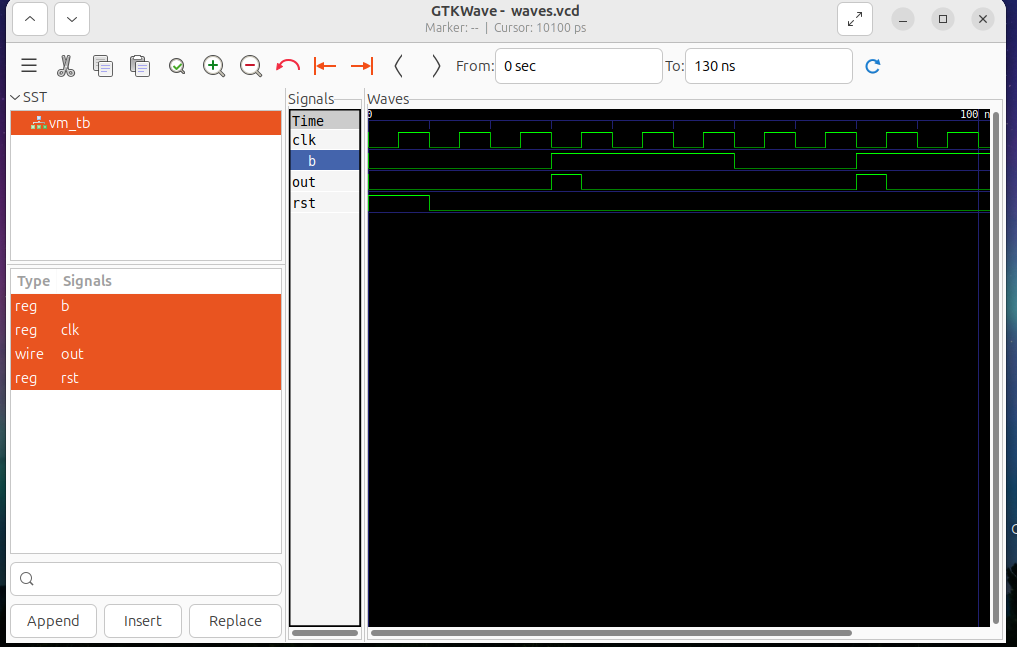
\includegraphics[width=1.0\linewidth]{images/23_gtkwave.png}
     \label{fig:rising_edge_waveform}
    \label{fig:placeholder}
\end{figure}


\vspace{0.5cm}

\section{RTL Synthesis using Yosys}

The RTL design was synthesized using Yosys. The Verilog source was read and the top-level module was selected for synthesis. The synthesis process performs RTL elaboration, process conversion, optimization, and FSM processing to obtain a gate-level representation of the design.


%----------------------------------------

%----------------------------------------
\section{Results and Observations}

\begin{itemize}
    \item The rising-edge detector was successfully implemented using a two-state, three-block FSM architecture.
    
    \item The output becomes HIGH for one clock cycle when the button input changes from LOW to HIGH.
    
    \item When the button remains HIGH, the output returns to LOW in the following clock cycle.
    
    \item The output remains LOW when there is no rising transition.
    
    \item The RTL functionality was verified through simulation using Icarus Verilog and GTKWave.
    
    \item The RTL design was synthesized using Yosys and subsequently passed through the OpenLane/OpenROAD physical-design flow.
\end{itemize}

\section{Conclusion}

A rising-edge detector using a digital push button was successfully designed using a three-block FSM architecture. The design detects a $0\rightarrow1$ transition and produces a single-clock-cycle output pulse. The functionality was verified through RTL simulation, and the design was synthesized .

\section{Sources of Error}

\begin{itemize}
    \item Incorrect state-transition logic may result in multiple or missing output pulses.
    
    \item Improper reset initialization can cause the FSM to begin in an undefined state.
    
    \item Incorrect clock-period or input timing in the testbench can lead to unexpected simulation results.
    
    \item In an actual push-button implementation, mechanical switch bouncing may produce multiple transitions. A debouncing circuit would be required for reliable hardware operation.
    
    \item Incorrect OpenLane configuration or clock constraints may prevent successful physical implementation.
\end{itemize}


\end{document}

